\documentclass[a4paper, 12pt]{report}
\textwidth = 14.5cm \textheight = 21.5cm \topmargin = -.5cm
\leftmargin = 5cm

\setcounter{secnumdepth}{2} \setcounter{tocdepth}{3}

%\oddsidemargin = 1cm
%\leftmargin = -3cm
%\evensidemargin = 5cm


%\includeonly{eqrmtech-h-apps}

\usepackage{amsmath}
\usepackage{graphicx}
\usepackage{fancybox}
\usepackage{natbib}
\bibliographystyle{grfchicago}
\usepackage{makeidx}
\usepackage{url}
\usepackage{psfrag}
\usepackage{supertabular}
\usepackage{drcaptionstyle}
\usepackage{listings}
%\usepackage{color}
\usepackage[usenames,dvipsnames]{color}
\usepackage{lscape}
\usepackage{multirow}
%\usepackage{bbding}
%\usepackage{epstopdf}

% set up some environments
\definecolor{light-gray}{gray}{0.8}
\lstset{basicstyle=\scriptsize}
%\lstset{frame=shadowbox, rulesepcolor=\color{blue}, fillcolor = \color{blue}} % create a frame and blue boundary for the xml file
\lstset{frame=single, backgroundcolor=\color{light-gray}}


\graphicspath{{diags/}}

\input eqrmtech-macros

\setlength{\parskip}{1em plus 0.1em minus 0.2em}
\setlength{\parindent}{0pt}


\makeindex



\title{EQRM: Geoscience Australia's Earthquake Risk Model\\
}

%\begin{center}
% Version 2.0
%\end{center}

\author{Technical Manual \\[1em]
Version 3.0 \\[3em]
David Robinson, Glenn Fulford and Trevor Dhu\\[1em]
Geoscience Australia}



\begin{document}
\maketitle

\pagenumbering{roman}

this is a blank page \newpage


this is a blank page
\newpage

 {\Huge \textbf{Acknowledgements}  }

The authors wish to thank John Schneider, leader of the Risk
Research Group at Geoscience Australia. John's expertise in the
areas of earthquake hazard and risk analysis have proven
invaluable throughout the project. Without his ongoing support and
advice the EQRM would not be half the product that it is today.

Andres Mendez from Aon Re in Chicago is acknowledged for providing
software that formed the backbone of the earthquake catalogue
generation. This generous contribution, as well as his high level
of collaborative support, was fundamental to the project's
success.

Bradley Horton is appreciated for the programming support that he
provided through a number of contracts with Ceanet. The
professionalism with which Bradley conducted his work extended
beyond the call of duty on many occasions. Bradley's efforts have
lead to great improvements in the useability and robustness of the
EQRM. Duncan Gray, Kurt Pudniks and Ken Dale, all of Geoscience
Australia, are also acknowledged for their coding efforts in
particular modules of the EQRM software.

The authors have sought advice on specific topics from a range of
people involved in the earthquake hazard and risk fields. The
following are acknowledged for their expertise and assistance;
George Walker of Aon Re, Professor John McAneney of Risk
Frontiers, Walt Silva of Pacific Engineering and Analysis, Don
Windeler and his team at Risk Management Solutions (RMS), Mike
Griffith at The University of Adelaide, Gary Gibson of the
Seismology Research Centre and Brian Gaull from Guria Consulting.

A number of people at Geoscience Australia have contributed
 to the development of the EQRM. Members of the Newcastle
and Lake Macquarie project team lead by Trevor Jones are
acknowledged for their assistance in shaping the early design of
the EQRM. Mark Edwards and Ken Dale are thanked for the countless
engineering questions that they have fielded over the four year
project. Matt Hayne, project leader of the Risk Assessment Methods
Project is thanked for creating the productive and supportive
environment that allowed this project to flourish. EQRM users,
Cvetan Sinadinovski, Annette Patchett, Ken Dale and Augusto
Sanabria are thanked for their feedback and for continually
inspiring the incorporation of new functionality. Ole Nielsen and
Duncan Gray are acknowledged for the provision of software
engineering advice and for generally improving the coding
abilities of the authors. Angie Jaensch, Greg Michalowski and
Fiona Watford are acknowledged for drafting some of the figures.
Finally, the authors wish to thank Adrian Hitchman, Ken Dale and
Augusto Sanabria for reviewing the drafts of this report. Their
reviews lead to substantial improvements to this manual.


\tableofcontents

\newpage
\pagenumbering{arabic}
\chapter{Introduction}
\label{ch:intro}

\section{Overview}

The EQRM application is a computer model for estimating earthquake
hazard and earthquake risk. Modelling earthquake hazard involves
assessing the probability that certain levels of ground motion
will be exceeded. Modelling of earthquake risk involves estimating
the probability of a building portfolio experiencing a range of
earthquake induced losses. For any number of synthetic
earthquakes, the EQRM application can be used to estimate:
\begin{enumerate}
\item the ground motion and its likelihood of occurrence
(earthquake hazard), \item the direct financial loss and its
likelihood of occurrence (earthquake risk), and \item less
reliably the number of casualties and injuries and their
likelihood of occurrence (earthquake risk).
\end{enumerate}

The EQRM application is Geoscience Australia's centerpiece for
modelling earthquake hazard and risk. Its use formed the basis for
Geoscience Australia's recent reports on Earthquake risk in the
Newcastle and Lake Macquarie \citep*{dr_Dhu02a} and Perth
\citep*{dr_Sinadinovski05a} regions.

The process for computing earthquake hazard can be described by
the following steps:
\begin{enumerate}
\item the generation of a catalogue of synthetic earthquakes (or
events) (see \cref{ch:source}), 
\item the propagation or
attenuation (see \cref{ch:atten}) of the `seismic wave' from each
of the events in 1 to locations of interest (see \cref{ch:application}),
\item accounting for the interactions between the propagating
`seismic wave' and the local geology or regolith (see
\cref{ch:reg}), and \item accounting for the probability of each
event and the estimation of hazard (see \cref{ch:risk}).
\end{enumerate}

The process for computing earthquake risk shares the same first
three steps as the earthquake hazard. The fourth step and onwards
can be described as follows:
\begin{enumerate}
\item[4.] estimating the probability that the portfolio buildings
(see \cref{ch:application}) will experience different levels of damage
(see \cref{ch:damage}), \item[5.] the computation of direct
financial loss as a result of the probabilities computed in 4 (see
\cref{ch:losses}), and \item[6.] assembling the results to compute
the risk (see \cref{ch:risk}).
\end{enumerate}

\section{Using this manual}

This manual describes the EQRM application; it has been designed
to serve the following three purposes:
\begin{enumerate}
\item describe the theory and methodology behind the EQRM
application; \item explain how to use the EQRM application to
model earthquake hazard and risk; and \item provide enough
information to assist those who may wish to access individual
modules and modify them.
\end{enumerate}

A number of features have been included to assist readers of the
manual. These features include:
\begin{itemize}
\item \textbf{Text highlighting -} Important parameters, file
names and code are identified by a typeset font. \item
\textbf{Index -} An index has been introduced to allow speedy of
navigation of the manual.

\end{itemize}


\section{About this manual}

\textit{\cref{ch:application}: The EQRM application} introduces
the EQRM software. The chapter describes the directory structure
and introduces important input parameter files. Setup and
operational processes are discussed and the conversion of the EQRM
to a stand-alone executable described. Readers who do not wish to
familiarise themselves with details of the EQRM application may
wish to skip this chapter.

\textit{\cref{ch:source}: Earthquake source generation} discusses
the creation of an earthquake catalogue. At the core of any hazard
or risk assessment is the simulation of synthetic earthquakes and
the creation of a catalogue of synthetic events. The chapter
describes how the simulation of earthquakes can focus around a
specific earthquake of interest (a scenario based simulation) or
how it can model the effect of `all foreseeable' events (a
probabilistic simulation).

\textit{\cref{ch:atten}: Ground-Motion Prediction Equations} discusses
the propagation (or attenuation) of the motion from each of the
synthetic earthquakes in the event catalogue to locations of interest.
Different measures of distance between an event and a site of interest
are introduced. The chapter also describes the attenuation models that
can be used with the EQRM application.

\textit{\cref{ch:reg}: Regolith amplification} discusses how local
geology, or regolith, can be incorporated in an earthquake hazard
or risk assessment. The chapter illustrates how the presence of
regolith can lead to amplification (or de-amplification) of both
ground and building motion, and consequently result in higher (or
lower) levels of hazard and risk.

\textit{\cref{ch:damage}: Building damage} describes how the EQRM
application estimates the probability that each building will
experience different levels of damage. The chapter gives a brief
discussion of the theory behind making such estimates as well as
outlining how to extrapolate the estimates to an entire portfolio
of buildings in a region of interest.

\textit{\cref{ch:losses}: Losses} illustrates how to model the
direct financial loss as a result of the damage estimates
described in \textit{\cref{ch:damage}}. The chapter also provides
a brief description of how the EQRM application can estimate
fatalities.

\textit{\cref{ch:risk}: Hazard and Risk Results}
describes how the results from the EQRM application can be
summarised and displayed. There are many ways to display estimates
of earthquake hazard and risk. Earthquake hazard is commonly
modelled in terms of a probability (often 10\%) of a particular
ground motion (usually acceleration) being exceeded in some time
frame (often 50 years). In the case of a scenario based
simulation, earthquake risk can be modelled in terms of dollar
estimates of building loss. In the case of a probabilistic simulation,
earthquake risk is often modelled in terms of one or both of the
following:
\begin{enumerate}
\item the loss per year averaged over a long period of time,
typically 10000 years. This is known as the annualised loss. \item
the probability that different levels of loss will be exceeded.
The plot of loss against such exceedance probabilities is referred
to as a probable maximum loss curve.
\end{enumerate}

\chapter{The EQRM application}
\label{ch:application}

The Earthquake Risk Model (EQRM) is capable of earthquake scenario
ground motion and scenario loss modeling as well as probabilistic
seismic hazard (PSHA) and risk (PSRA) modeling. It is a product of
Geoscience Australia, an Australian Government Agency.

This chapter describes the EQRM application. Input files and
parameters are discussed and directions on how to run the EQRM
provided. Readers who are interested in only the EQRM methodology
and not the EQRM software package may wish to skip this chapter.

\section{EQRM inputs}

The input files required by the EQRM depend on the nature of the
simulation conducted. For example, the inputs for a scenario loss
simulation are different to those required for a probabilistic
seismic hazard analysis. \tref{tab:input-overview} provides a
summary of the inputs required by the EQRM. The EQRM Demos (see
\sref{sec:application-demo}) provide examples of each input file and
demonstrate how to run the EQRM for each of the four main simulation
types. srefmulti provides an overview of each of the main input
files. Further details are provide in the following chapters.

\begin{table}
\caption{Input files required for different types of simulation with
the EQRM. The astericks indicates optional input files, the
requirement for which depends on settings in the EQRM control file
(see \cref{ch:reg} for more information).}
\label{tab:input-overview} \centering
\begin{tabular}{|l|l|l|}
\hline
 & \textbf{hazard} & \textbf{risk} \\
\hline
\textbf{scenario} & EQRM controlfile & EQRM controlfile \\
  & amplification factors* & amplification factors* \\
  & hazard grid & building database \\
\hline
\textbf{probabilistic} & EQRM controlfile & EQRM controlfile\\
  & source file(s) & source file(s) \\
  & event type controlfile & event type controlfile \\
  & amplification factors* & amplification factors* \\
  & hazard grid & building database \\
\hline
\end{tabular}
\end{table}

It contains a series of input parameters and flags that must be set
by the user. \sref{sec:application-parfiles} describes other files
that are required by the EQRM modules.

\subsection{The EQRM control file}
\label{sec:application-EQRMcf}

% First lets include the descriptom of the EQRM control file and its parameters
\input param_list_text

% Now lets include an example EQRM controlfile

\clearpage For example, the following grey shaded box provides an
example of an EQRM controlfile to undertake a PSHA. It is actually
one of the demos described in more detail in
\sref{sec:application-demos}.

\lstinputlisting{../../demo/setdata_ProbHaz.py}


\clearpage
\subsection{The source files}

\lstinputlisting{xml_examples/source_model_zone_example.xml}



\subsection{Parameter files}
\label{sec:application-parfiles}

This section identifies the important input files that are used by
different components of the EQRM. Input files can be dependent or
independent of region. For example the file
 \typeparfile{newc}{\_par}{\_ampfactors}{.mat} contains the amplification factors
for the Newcastle region (see \sref{ch:reg}), whereas the file
 \typeparfile{attn\_toro}{\_midcontinent}{\_momag}{.txt}
contains attenuation coefficients for the \citet*{dr_Toro97a}
attenuation model (see \sref{ch:atten}) which are not dependent on
region. The EQRM identifies the desired region dependent files
using the user defined parameter \typepar{site}{\_loc}{} (see
\sref{sec:application-setdata}).

The EQRM makes use of default data to reduce the need for a large
number of defined input files. Default data files are stored in
the directory \typedir{*/eqrm/eqrm\_app}{/resources}{/data} (see
\sref{sec:app-dirstruct}). The EQRM facilitates the use of
non-default data by first looking in the user defined
 \typepar{inp}{ut}{dir} (see \sref{sec:application-setdata}) for
required files. If the required files are found in
 \typepar{inp}{ut}{dir} they will be used by the EQRM, if the files
are not found in  \typepar{inp}{ut}{dir} then the default files
are used.

Note that default files are available for pre-defined regions
only. For example; Newcastle and Perth region default data can be
accessed by defining \typepar{site}{\_}{loc} of \typenewc and
\typeperth respectively.

\begin{table}
\caption{Default parameter files in
\typedircaption{*/eqrm/eqrm\_app}{/resources}{/data}.}
\label{tab:app-inputfiles} \vspace{0.8em}
\begin{tabular}{|l|p{0.7\textwidth}|}
\hline
Chapter & Files \\
\hline Earthquake & $\typeparfile{<site\_loc>}{\_par}{\_sourcepolys}{.txt}$ \\
Source generation &  $\typeparfile{<site\_loc>}{\_par}{\_sourcezones}{.txt}$ \\
\hline
Grids and & $\typeparfile{au}{s}{\_mat}{.txt}$\\
building & $\typeparfile{aust}{ralia}{\_bndy}{.txt}$\\
databases & $\typeparfile{<site\_loc>}{\_par}{\_site}{.mat}$\\
 &  $\typeparfile{<site\_loc>}{\_par\_site}{\_uniform}{.mat}$ \\
 &  $\typeparfile{<site\_loc>}{\_par\_study}{\_region\_box}{.txt}$ \\
  & $\typeparfile{sitedb}{\_<site}{\_loc>}{.mat}$ \\
 & $\typeparfile{suburb}{\_post}{code}{.csv}$\\
  & $\typeparfile{text}{b}{types}{.txt}$ \\
 & $\typeparfile{text}{busage}{FCB}{.txt}$ \\
 &  $\typeparfile{text}{b}{uses}{.txt}$ \\
\hline
Attenuation & $\typeparfile{attn}{\_atkboore}{\_momag}{.txt}$\\
 &  $\typeparfile{attn\_sadigh}{\_coeff\_momag}{\_great65}{.txt}$ \\
 &  $\typeparfile{attn\_sadigh}{\_coeff\_momag}{\_less65}{.txt}$ \\
 &  $\typeparfile{attn\_somer}{\_nonrift}{\_hori}{.txt}$ \\
 &  $\typeparfile{attn\_somer}{\_nonrift}{\_vert}{.txt}$ \\
 &  $\typeparfile{attn\_somer}{\_rift}{\_hori}{.txt}$ \\
 &  $\typeparfile{attn\_somer}{\_rift}{\_vert}{.txt}$ \\
 & $\typeparfile{attn\_toro}{\_midcontinent}{\_momag}{.txt}$,              \\
\hline
Regolith &  $\typeparfile{<site\_loc>}{\_par}{\_ampfactors}{.mat}$\\
amplification &  $\typeparfile{<site\_loc>\_par}{\_site\_class}{\_mask}{.mat}$ \\
 &  $\typeparfile{<site\_loc>\_par}{\_site\_class}{\_polys}{.mat}$ \\
\hline
Building & $\typeparfile{b}{factors}{db}{.mat}$\\
damage & $\typeparfile{bfactors}{db}{\_hazus}{.mat}$ \\
 & $\typeparfile{bfactors}{db}{\_wshop}{.mat}$ \\
 & $\typeparfile{bfactorsdb}{\_wshop}{\_update2}{.mat}$ \\
 & $\typeparfile{bfactorsdb}{\_wshop}{\_update3}{.mat}$ \\
 & $\typeparfile{factors}{-nonstruct}{dam}{.csv}$ \\
 &  $\typeparfile{factors}{-struct}{dam}{.csv}$ \\
\hline
Losses & $\typeparfilelong{rc\_perRepl}{CostwrtBuildC}{EdwardsFCBusage}{.mat}{rc\_perRepl...EdwardsFCBusage}$ \\
& $\typeparfilelong{rc\_perReplCost}{wrtBuildCEdwards}{Hazususage}{.mat}{rc\_perRepl...EdwardsHazususage}$\\
% & $\typeselfnoindex{rc\_perReplCost}{wrtBuildCEdwards}{Hazususage.mat}\index{\scriptsize\texttt{rc\_perReplCostwrtBuildCEdwardsHazususage.mat}\normalsize}$\\
& $\typeparfile{rc\_perReplCost}{wrtBuildC}{Hazusage}{.mat}$\\
& $\typeparfile{econ}{\_p}{ar}{.mat}$\\
\hline
\end{tabular}
\end{table}

\tref{tab:app-inputfiles} summarises the important input files
that can be found in the default data area. The files are listed
against the chapter where more information can be found.


\subsection{Running the EQRM in MATLAB}
\label{app:runEQRM}


The EQRM has a special startup function
(\typefunc{eqrm}{\_start}{up}) that adds all the required
directories to the MATLAB path. The following instructions
describe how to use \typefunc{eqrm}{\_start}{up} to set the MATLAB
path:
\begin{itemize}
\item move to the directory
\typedir{*/eqrm/eqrm\_app}{/m\_code}{/startup} \item at the
command line type \newline \texttt{>>
eqrm\_startup\indexfunc{eqrm\_startup}(`*$\backslash$eqrm$\backslash$eqrm\_app')}
\end{itemize}

The EQRM has a special GUI known as the
\typegui{eqrm}{\_param}{\_gui} that can be used to create a
\typeself{set}{da}{ta} file, run the EQRM application or analyse
the EQRM outputs. To launch the GUI simply type the following at
the command line:
\begin{itemize} \item[\texttt{>>}] \texttt{eqrm\_param\_gui}\indexgui{eqrm\_param\_gui} \end{itemize}
It is beyond the scope of this manual to discuss the
\typeself{eqrm}{\_param}{\_gui} further. However it is user
friendly and reasonably self explanatory. Alternatively the EQRM
can be run from the command line using the function
\typefunc{eqrm}{\_analy}{sis}. To find out how to use
\typefunc{eqrm}{\_analy}{sis} type the following at the MATLAB
command line: \begin{itemize} \item[\texttt{>>}] \texttt{help
eqrm\_analysis}
\end{itemize}

The EQRM has a special Output Manager GUI that can be used to
view, analyse and plot EQRM outputs. The Output Manager is also
known as the Data Interrogation Tool
(DIT)\index{DIT}\index{GUI!DIT}\index{Data Interrogation
Tool}\index{GUI!Data Interrogation Tool}. A report generation
facility has been included with the Output Manager and can be used
to create a \LaTeX \texttt{*.tex} file with EQRM output figures.
The \LaTeX file can be compiled into a \texttt{.ps} and/or
\texttt{.pdf} file if the appropriate MikTeX software is
installed.


\subsection{Compiling and using a stand--alone version of the EQRM in MATLAB R14SP1}

Using the MATLAB compiler it is possible to create a stand--alone
version of the EQRM that can be used without requiring MATLAB. The
instructions for MATLAB R13 are given in \aref{app:MATLABR13}.

\section{Creating a stand--alone executable of the EQRM GUI in MATLAB R14SP1:}
\label{app:MATLABR13}

Type the following at the MATLAB command line for the source
machine \begin{itemize} \item[\texttt{>>}]
\texttt{cnt\_do\_mcc\_build\_to\_system(`eqrm\_param\_gui',<*/path>)}
\end{itemize}

This process will create the following files in \texttt{<*/path>}:
\begin{enumerate}
\item \typeselfnoindexnoline{eqrm}{\_param}{\_gui.exe};  \item a
directory named \typeselfnoindexnoline{eqrm}{\_param}{\_gui\_mcr};
and \item \typeselfnoindexnoline{eqrm}{\_param}{\_gui.ctf}.
\end{enumerate}

\vspace{2em}

\textbf{Prepare the files for transportation as follows:}
\begin{enumerate} \item Create a folder entitled
\typeselfnoindexnoline{*/te}{st}{exe}. \item In
\typeselfnoindexnoline{*/te}{st}{exe} create two folders
 \typeselfnoindexnoline{*/}{testexe}{/system} and
 \typeselfnoindexnoline{*/}{testexe}{/mcr}.
\item Copy  \typeselfnoindexnoline{eqrm}{\_param}{\_gui.exe},
\typeselfnoindexnoline{eqrm}{\_param}{\_gui\_mcr} and
\typeselfnoindexnoline{eqrm}{\_param}{\_gui.ctf} (created above)
into \typeselfnoindexnoline{*/}{testexe}{/system}. \item Copy the
following files from \typeselfnoindexnoline{*/EQRM}{ROOT}{/system}
into \typeselfnoindex{*/}{testexe}{/system}:
\begin{enumerate}
\item \typeselfnoindexnoline{root\_mat}{\_creator}{\_cnt.exe};
\item the directory
\typeselfnoindexnoline{root\_mat}{\_creator}{\_cnt\_mcr}; and
\item \typeselfnoindexnoline{root\_mat}{\_creator}{\_cnt.ctf}.
\end{enumerate}
\item Copy \typeself{\_MCR}{Instal}{ler.exe} from
\typeselfnoindexnoline{<MATLABROOT>/toolbox}{/compiler/deploy}{/win32/MCRInstaller.exe}
into \typeselfnoindexnoline{*/}{testexe}{/mcr}. \item Copy the
directory \typeselfnoindexnoline{*/EQRM}{ROOT}{/resources} to
\typeselfnoindexnoline{*/}{testexe}{/resources}.
\end{enumerate}

\vspace{2em} \textbf{Installation onto the target machine is
achieved as follows:}
\begin{enumerate}
\item Move the contents of \typeselfnoindex{*/te}{st}{exe} onto
the target machine. \item Run \typeself{\_MCR}{Instal}{ler.exe} on
\typeselfnoindex{*/}{testexe}{/mcr} by double clicking on it.
\item Set environment path on the target machine
\begin{enumerate}
\item open the control panel; \item open system; \item select the
advanced tab; \item select environment variables; \item create new
user variable entitled \typeselfnoindex{p}{a}{th}; \item add the
following path names (separated by semi colons) into the value
field for \texttt{path};
\begin{itemize} \item
\typeselfnoindexnoline{*/}{testexe}{/system}; and \item
\typeselfnoindexnoline{*/testexe}{/mcr/v71}{runtime/win32};
\end{itemize}
\item Log off and log back on.
\end{enumerate}
\item Set the software path as follows
\begin{enumerate}
\item Open a DOS shell; \item Type
\typeselfnoindex{root}{\_mat\_creator}{\_cnt.exe}; \item On the
`EQRM root file creation' GUI select the EQRM root directory (i.e.
\typeselfnoindex{*/te}{st}{exe}).
\end{enumerate}
\item Open the EQRM GUI by typing
\typeselfnoindex{eqrm}{\_param}{\_gui.exe} at the DOS command
prompt.
\end{enumerate}

\chapter{Earthquake source generation}
\label{ch:source}

\section{Overview}

The EQRM conducts probabilistic seismic hazard analysis (PSHA) and
probabilistic seismic risk analysis (PSRA) using an event based
approach. This means that the ground motions (hazard) and loss
(risk) are computed for each event individually and the results
separately aggregated to form probabilistic estimates. The event
based approach differs from the traditional approach to PSHA which
integrate over all magnitude and distance combinations to attain
probability levels for exceeding a particular level of ground
motion in a pre-defined period of time. The traditional approach
is introduced by \citet{dr_Cornell68a} and summarised by
\citet{dr_McGuire90a}. A core component of any event based
analysis with the EQRM is the generation of a simulated
event\index{simulated event} (or earthquake) catalogue. The
generation of the earthquake catalogue relies upon an existing model for
the seismicity in the region. Typically the  model of seismicity comes
 from an interpretation of historical earthquakes,
 geology and neotectonics. The current version of the EQRM application requires a source model
that consists of a set of areal source zones (defined by a polygon) with associated
Gutenberg-Richter recurrence relationships and the option of including fault sources (defined by a plane) with associated 
Gutenberg-Richter or characteristic earthquake recurrence relationships \citet{dr_Schwartz84}. 

\emph{Areal source zones} typically capture the background seismicity in an area and are decribed by the acitivty rate within
each source zone through its Gutenberg-Richter \emph{a} and \emph{b} values. In event-based PSHA calculations, such as \typeself{E}{QR}{M},
synthetic ruptures will be generated stochastically throughout the areal source zone. However, a user may have sufficient information 
on the geometry and earthquake recurrence rates of a known fault and may want to place synthetic ruptures on the fault by defining a 
\emph{fault source}. In this instance, instead of placing the synthetic ruptures within the areal source zone, they will be placed 
on the known fault plane. \\

In addition, a novel technique has been developed to generate synthetic ruptures within a 3D volume that may represent seismotectonic 
features such as the intraplate environment of a subducting slab. Such events are often referred to as intraslab earthquakes and have been known
to generate larger and devastating earthquakes (e.g. 30 September 2009 Padang earthquake in Indonesia). \\

This chapter describes the process of creating an earthquake catalogue for probabilistic seismic hazard 
analysis and for defining an individual scenario event. The chapter is organised as follows. First the 
method of generating realistic ruptures in source zones and fault zones is discussed in Section \label{sec:source-EQgeom}. Second, the approach for 
determining recurrence rates is presented in Section \label{sec:source-EQrec}. Lastly, Section \label{sec:source-scen} 
describes scenario event generation.

\section{Creating an earthquake catalogue for probabilistic seismic hazard analysis}% a probabilistic seismic hazard analysis}
\label{sec:source-EQcat}

This section describes the method to generate a synthetic earthquake catalog of plausible events. The event catalog can be
created for events that are defined within an areal source or located on a known fault source. The recurrence relationship for the events
can be defined as a Gutenberg-Richter or Characteristic earthquake relationships.

A simulated event\index{simulated event} is represented by a plane
(or rupture) in 3D space that signifies the region where slip has
occurred. The geometry of a rupture plane is shown in
\Fref{fig:hrupture-3d}. The important parameters of a simulated
event\index{simulated event} are its location, geometry, magnitude
and activity (or likelihood of occurrence). The rupture trace is
the surface projection of the simulated event\index{simulated
event} along the direction of dip. The position and geometry of
the rupture trace is defined by its start $(r_s^{lat},r_s^{lon})$
and end $(r_e^{lat},r_e^{lon})$ points, its azimuth $r_{azi}$ and
its length $r_l$. The position and geometry of the rupture plane
are defined by its width $r_w$, dip $r_{dip}$ and the position of
its centre (or rupture centroid). The rupture centroid is defined
in cartesian coordinates $(r_x,r_y,r_z)$ in km using a local
coordinate system with origin at the rupture start point (see
\Fref{fig:hrupture-3d}). The orientation of the local coordinate
system is such that the $x-axis$ is oriented along the rupture
trace with positive direction pointing towards the rupture end
point, the $z-axis$ is pointing vertically downwards and the
$y-axis$ is oriented along the surface of the `earth' such that
the axes form a right handed triad. The vertical projection of the
rupture centroid is also described by its latitude $r_c^{lat}$ and
longitude $r_c^{lon}$. The event magnitude is represented as a
moment magnitude and is generated by the process described in
\sref{sec:magnitude_selection}. The activity (or likelihood of
occurrence) of the simulated event\index{simulated event} is
described by the event activity which represents the number of
times a given simulated event\index{simulated event} (conditional
on magnitude and position) occurs in one year (see
\sref{sec:magnitude_selection}).

\begin{figure}[htp]
\begin{center}
\begin{tabular}{ll}
(a) & (b) \\
% \psfrag{Fault Trace}{Rupture Trace} \psfrag{Dip}{$r_\theta$}
% \psfrag{Azimuth}{$r_\phi$}
\includegraphics[width=0.49\textwidth]{diags/fig-hrupture-3d} &
\includegraphics[width=0.41\textwidth]{diags/fig-hrupture-2d}
\end{tabular}
\end{center}
\caption{Orientation and dimension of the rupture plane in (a) 3D
and (b) 2D vertical projection to ground surface.}
\label{fig:hrupture-3d}
\end{figure}




\begin{table}
\centering \caption{Columns in \typevarcaption{ev}{nt}{db}. Note
that some of the columns are not defined until after
\typefunccaption{fuse}{4}{\_hzd} is run (see
\sref{source:spawning}).}
 \label{tab:evntdb-columns}
\vspace{0.8em}
\begin{tabular}{r|p{0.85\textwidth}}
\hline
column & description \\
\hline
1 & an integer corresponding to the generation source zone from which this event was generated \\
2 & $r_s^{lat}$ - latitude of rupture trace start point (decimal degrees)\\
3 & $r_s^{lon}$ - longitude of rupture trace start point (decimal degrees)\\
4 & $r_e^{lat}$ - latitude of rupture trace end point (decimal degrees)\\
5 & $r_e^{lon}$ - longitude of rupture trace end point (decimal degrees)\\
6 & $r_\phi$ - azimuth of rupture trace (decimal degrees from True North)\\
7 & $r_{dip}$ - dip of rupture plane (0 $<$ decimal degrees $<$ 90 from the surface) \\
8 & $A_{min}$ - number of earthquakes of magnitude $m_{min}$ or greater per year\\
9 & integer pointer to attenuation model for use with the synthetic earthquake.\\
10 to 18 & place holder (currently not used) \\
19 & $w_e$ - weight derived from event spawning  \\
20 & $r_\nu$ - event activity (the number of magnitude $r_m$ earthquakes expected per year scaled to the number being simulated) \\
21 & $r_m$ - event magnitude (moment magnitude)\\
22 & $r_\varepsilon$ - source epsilon from event spawning\\
23 & $r_c^{lat}$ - latitude of event centroid (decimal degrees) \\
24 & $r_c^{lon}$ - longitude of event centroid (decimal degrees) \\
25 & $r_z$ - event centroid depth z (km from ground surface) \\
26 & $r_x$ - event centroid x (km along rupture trace from the
start of trace) \\
27 & $r_y$ - event centroid y (km perpendicular from trace in
direction of
dip) \\
28 & $r_l$ - length of rupture (km) \\
29 & $r_w$ - width of rupture (km measured along dip) \\
30 & a unique integer for each synthetic earthquake in the generation zone (polygon). Note that the integer count begins again for each generation zone. \\
31 & place holder (currently not used) \\
\hline
\end{tabular}
\end{table}


\subsection{Simulated events and virtual fault\index{virtual fault}s}

The terms simulated event\index{simulated event}, simulated
earthquake\index{simulated earthquake} and simulated
rupture\index{simulated rupture} are congruent and will be used
interchangeably throughout this document. Sometimes the adjective
`simulated' will be omitted for brevity. An adjective `actual'
will be used in place of `simulated' to refer to a historic
earthquake (i.e. one that has actually occurred rather than one
that is simulated).

A virtual fault\index{virtual fault} refers to a plane in 3D space upon which an event can
occur.  The virtual fault can be located in within an areal source or defined by a known fault. 
The \typeself{E}{QR}{M} works by first creating a virtual fault\index{virtual fault}, either within an
areal source zone, or by a user defined know fault. The rupture is then placed 
on the virtual fault\index{virtual fault} (the
rupture is not allowed to exceed the bounds of the virtual
fault\index{virtual fault}). The introduction of a virtual
fault\index{virtual fault} is the mechanism by which the
\typeself{E}{QR}{M} application constrains the location and extent
of each rupture. The depth to the top of a virtual
fault\index{virtual fault} is defined as the depth to the
seismogenic region $f_z$ (see
\tref{tab:site-loc-par-sourcezones}). Other geometrical parameters
of virtual fault\index{virtual fault}s include the width $f_w$ and
length $f_l$. 


\subsection{Location of synthetic earthquakes in areal sources}
\label{sec:rup-location}

The location of each event is assigned randomly within an areal source zone 
and on a fault source. 
This assignment is done in such a way that the event has
an equal probability of being located anywhere in the `generation
polygon' or on the fault. 

The first phase of locating the events involves positioning the
centre point of each rupture trace ($r_c^{lat}$,$r_c^{lon}$). A
rectangular box is generated over the top of the source zone polygon. The
box is bounded by the minimum and maximum latitude and the
minimum and maximum longitude of the source zone itself. 

% Need to change this to have no underlying grid. 
\begin{figure}
\begin{center}
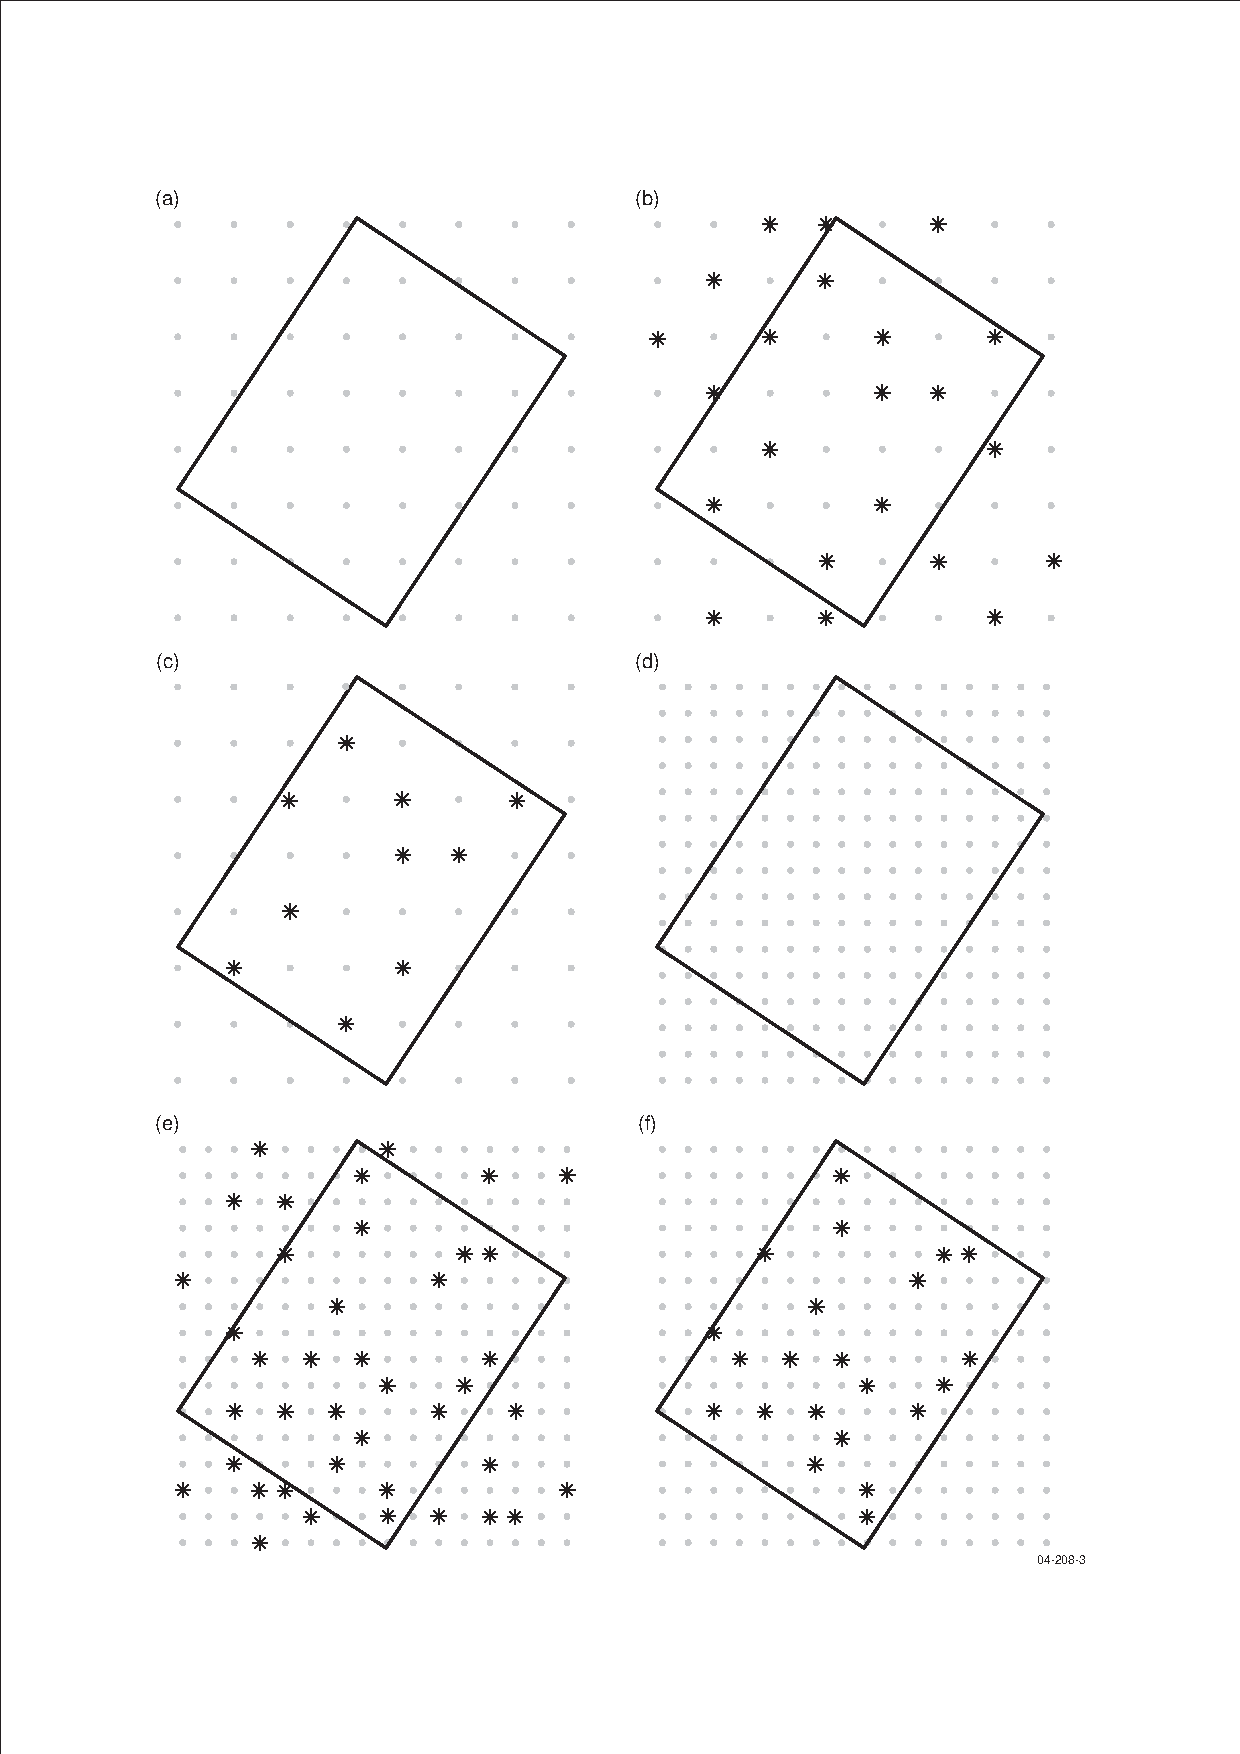
\includegraphics[width=0.9\textwidth]{fig-hsource-trace-starts}
\end{center}
\caption{Random selection of rupture centroids for a
rectangular `generation polygon'. (a) to (c) illustrate the first
iteration and (d) to (f) the second iteration after contraction of
the grid spacing.} \label{fig:source-trace-starts}
\end{figure}

The rupture centroid of each event is then randomly placed within the box 
using a discrete uniform probability density function
(\fref{fig:source-trace-starts}b). The event is the checked to identify whether 
it falls within the source polygon or not. Events that fall within the source polygon 
are kept and those that lie outside it are discarded. 

The second phase of locating events involves positioning the start and end
point of the rupture trace. Assume for the moment that both the
length and azimuth of the rupture trace are already known (see
\sref{sec:dim-rupture} and \sref{sec:az-dip-rupture} respectively
for a description of how these are computed). It is then a trivial
process to compute the start and end of the rupture trace
$(r_s^{lat},r_s^{lon} and r_e^{lat},r_e^{lon})$. It is important to note that the \typeself{E}{QR}{M} will allow the 
start or end points of the rupture trace to lie outside of the source polygon 
providing the rupture centroid is located within the polygon. The source zone polygon 
is only used to constrain the rupture centroid ($r_c^{lat},r_c^{lon}$).

\subsection{Location of events on fault sources}

As discussed earlier in this chapter, fault sources in the \typeself{E}{QR}{M} can represent three different styles of faulting:

\begin{itemize}
\item Crustal faults
\item Subduction interface faults
\item Intraslab faults in the subducting slab
\end{itemize}

The method for placing synthetic ruptures on crustal faults and subduction interface faults is the same, but intraslab faults required a 
different approach. \\

\subsubsection{Crustal Faults and Subduction Interface Faults}
Assuming again that we have already defined the length and width of the rupture plane, we then solve to find the location of the rupture
trace along the predefined fault trace by:

\begin{equation} \label{eq:ds}
D_s = (f_l - r_l) \times \mathtt{X}
\end{equation}

where $\mathtt{X}$ is a random variable between 0$\rightarrow$1. Following this step the new start and end of the rupture trace can be 
obtained using the rupture length, azimuth of the fault. \\

We now use $D_s$ from equation \ref{eq:ds}, and the precalculated rupture length and fault azimuth to calculate the 
new longitude and latitude of the start and end of the rupture trace (\ref{fig:traces}). 

% \begin{figure}[htp]
% \centerline{\includegraphics[width=6cm]
% {faulttrace.png}}
% \caption{A plan view of the fault trace and rupture trace defined by its start and end coordinates.}
% \label{fig:traces}
% \end{figure}

We now follow a similar process (to equation \ref{ds}) to determine the depth of the rupture centroid. Since we 
already have the fault width we can randomly assign the depth of the rupture centre while making sure the rupture 
plane does not extend beyond the top and bottom of the fault plane defined in the source file (\ref{fig:rzrange}). 

% \begin{figure}[htp]
% \centerline{\includegraphics[width=12cm]
% {depthrange.png}}
% \caption{A schematic diagram of how we define the depth range of the rupture centroid.}
% \label{fig:rzrange}
% \end{figure}

We first find the depth range which the rupture centroid can lie within [$r_z^{min}, r_z^{max}$] such that 
the rupture plane does not extend above or below the bounds of the seismogenic zone [$f_z^{top}, f_z^{bot}$]:

\begin{subequations} \label{drange}
\begin{align}
r_z^{min} & = \mbox{minimum depth of rupture centroid}  \\
r_z^{max} & = \mbox{maximum depth of rupture centroid}   \\
r_z^{min} & = r_z^{top} + 0.5r_w  \times sin(r_\theta  \times \mbox{rad})    \\
r_z^{max} & = r_z^{bot} - 0.5r_w  \times sin(r_\theta \times \mbox{rad})  
\end{align}
\end{subequations}

where $f_\theta = r_\theta$. Note that for intrapate ruptures which will be discussed later $f_\theta \ne r_\theta$. 
We can now randomly assign the rupture centroid depth using a uniform distribution between $r_z^{min}$ and $r_z^{max}$ 
using the \texttt{numpy} package in \texttt{python}:

\begin{equation} \label{eq:rand}
	r_z = ( r_z^{max}-r_z^{min} ) \times  \mathtt{X} +   r_z^{min}
\end{equation}

where $\mathtt{X}$ is a random varaible from 0$\rightarrow$1. The local x and y coordinates ($r_x$ and $r_y$) of the rupture 
centroid can be calculated by the employing the same equations as for the source zones:

\begin{equation}
r_y = r_z  \frac{cos(f_\theta  \times rad)}{sin(f_\theta  \times rad)}
\end{equation}

\begin{equation}
r_x = \frac{r_l}{2}
\end{equation}

Where the rupture centroid location in local coordinates ($r_x$, $r_y$) can be converted to longitude and latitude ($r_c^{lon}$, $r_c^{lat}$).

\subsubsection{Intraslab Faults}

The concept of creating realistic ruptures that represent events in a subducting slab is achieved by considering these events as 
out of plane ruptures. The subducting slab is defined as a 3D plane from which rupture planes extend out from at angles defined by
the user (FIGURE PLOT). For this functionality and out of dip value must be defined ($\delta_\theta$). 
This parameter defines the angle between the dipping fault and the rupture plane (figure \ref{fig:intraslabGeom}). If the rupture 
plane is parallel to the fault plane this value will be zero. If the rupture plane is it an angle to the dipping plane then it 
will be non-zero. When handling a non-zero $\delta_\theta$ we also need to consider another parameter, $\Delta_\theta$, which 
defines the range of dips we will sample across to obtain the rupture dip ($r_\theta$, figure \ref{fig:intraslabGeom}).
We first take a uniform sample from the range [$\delta_\theta - \Delta_\theta, \delta_\theta + \Delta_\theta$]  to determine 
the out of plane angle ($\omega$) and the dip of the rupture plane ($r_\theta$) :


\subsection{Overlapping source zones}

The concept of overlapping zones in a source model is useful for
accommodating background seismicity. In principle, the code can
accommodate overlapping seismic zones, i.e. where two seismic
zones share a common geographical region. However, it should be
noted that earthquakes will be distributed randomly in the common
region for each zone that exists. That is, a simulation using
overlapping source zones (such as that shown in
\fref{fig:h-source-overlapping}(a)) may lead to a greater number
of simulated earthquake\index{simulated earthquake}s in the common
region than may be warranted by the source model. This only poses
a problem if the recurrence relationship (i.e. the $a$, $b$
parameters) being used has not been modified to account for the
`double counting' in the simulated catalogue (generally this will
not have been done). To overcome this problem, it is advisable to
define the source zones in such a way that there are no
overlapping regions. \fref{fig:h-source-overlapping} demonstrates
two different techniques that can be used to incorporate
overlapping source zones in the EQRM. Both of the illustrated
techniques are based on creating a doughnut.

\begin{figure}[htp]
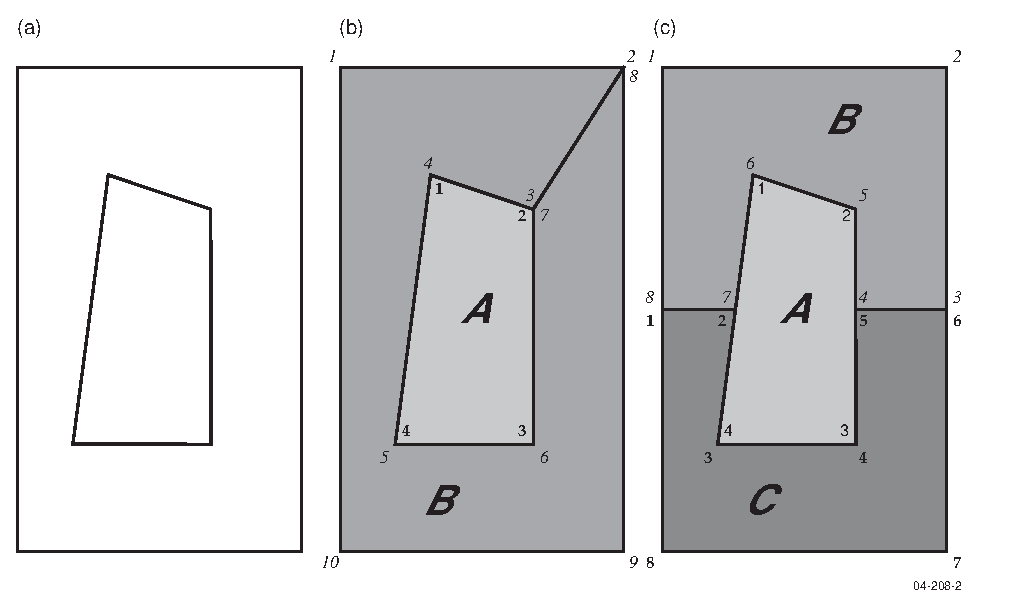
\includegraphics[width=1\textwidth]{fig-hsource-overlapping-zones}
\caption{Overlapping source zones shown in (a) can be incorporated
into the EQRM by cutting out a doughnut (b) or splitting the outer
polygon (c). The numbers in different fonts illustrate how the
polygon vertices could be listed in the
\typeparfilecaption{<site\_loc>}{\_par\_source}{zones}{.txt} file.
} \label{fig:h-source-overlapping}
\end{figure}



\subsection{Magnitude selection and event activity}
\label{sec:magnitude_selection}

A `stratified' Monte-Carlo technique is used to assign the event
magnitudes. The stratified nature of the technique ensures that
the full range of magnitudes is adequately sampled. The stratified
Monte-Carlo technique is illustrated in
\fref{fig-hattn-montecarlo} for the general case. This approach is
distinctly different to a brute force Monte-Carlo technique that
would preferentially sample the more probable lower magnitude
events. Such an approach would require the sampling of a large
number of small events to ensure that a handful of large events
are sampled.

The algorithm described in this section is the algorithm applied
when a single source model is used and the `generation
polygons'\index{generation polygon} are the source zones of the
source model. Some minor modifications are required when multiple
source models are used or the `generation
polygons'\index{generation polygon} differ from the source zones.
These modifications are described in \sref{sec:source-multizones}.


\begin{figure}[htp]
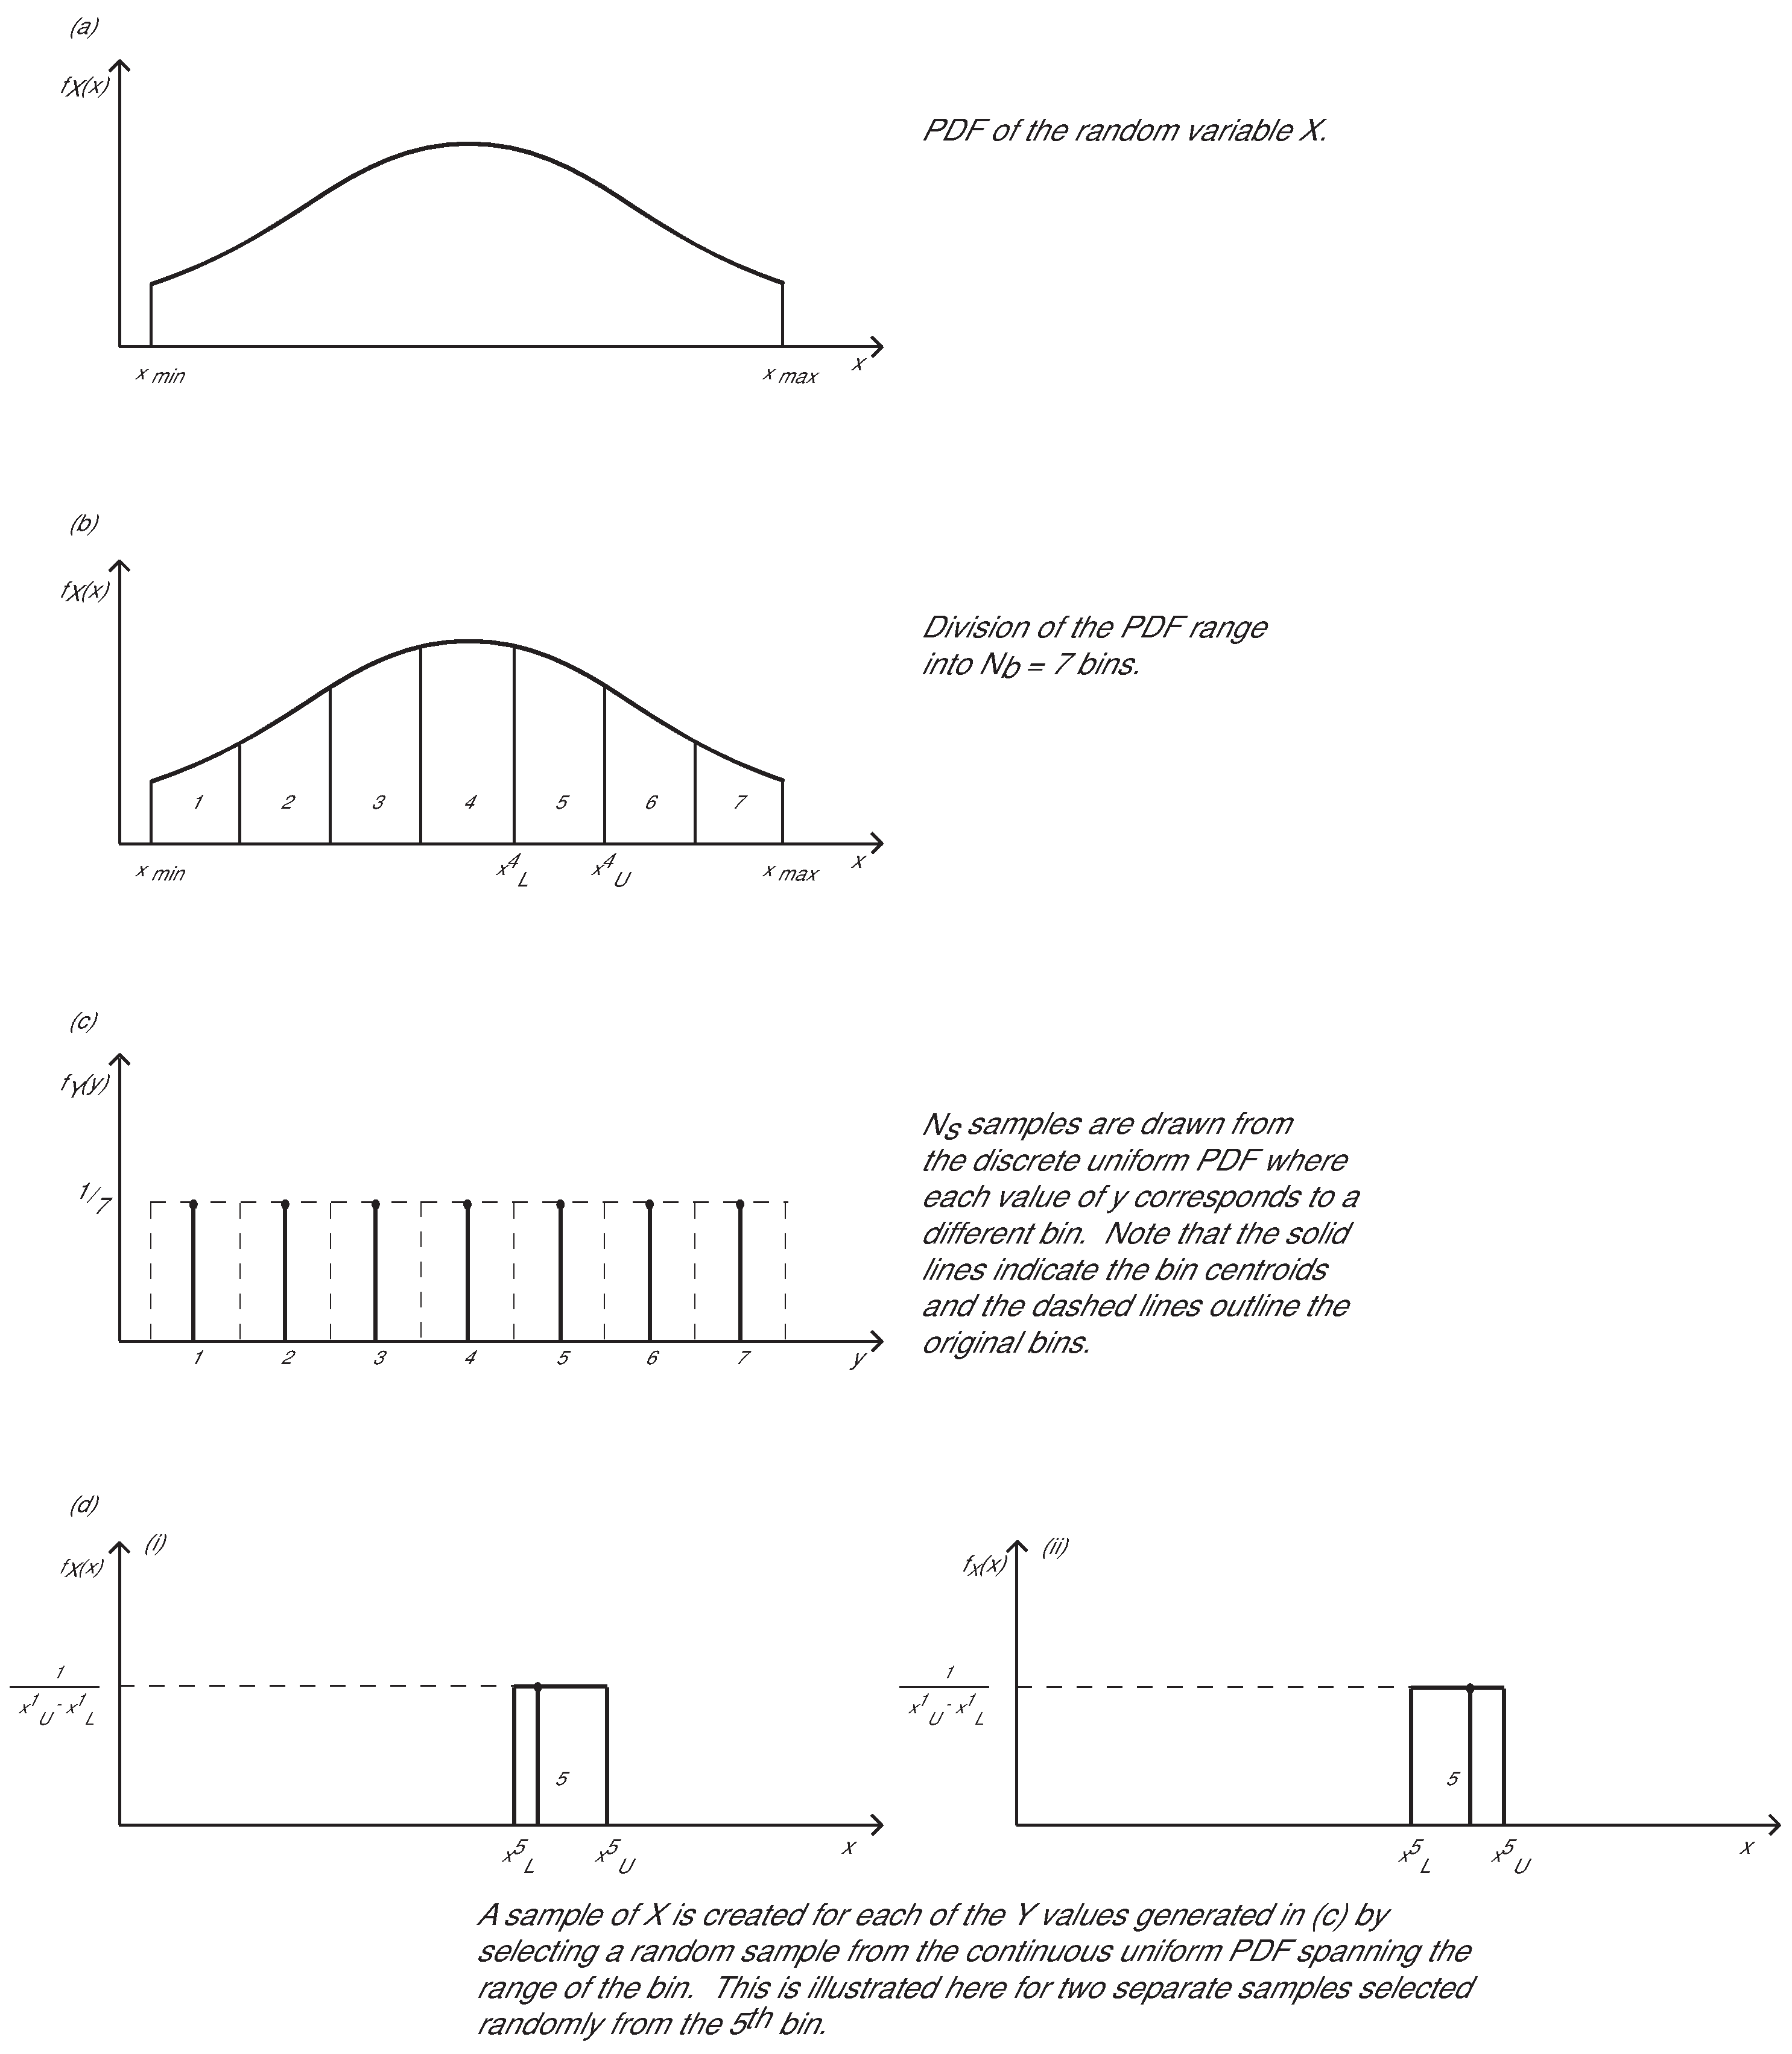
\includegraphics[width=1\textwidth]{fig-hattn-montecarlo}
\caption{Stratified Monte Carlo technique for sampling a PDF. In
this case a normal distribution is shown but any PDF can be used.}
\label{fig-hattn-montecarlo}
\end{figure}

The Probability Density Function (PDF) for the event magnitudes is
based on the bounded Gutenberg-Richter law \citep{dr_Kramer96a}.
The EQRM application simulates a number $N_s$ of earthquake
events. Considering the $i^{th}$ source zone, the algorithm for
choosing the magnitude of each event can be summarised as follows:

\begin{enumerate}
\item Bound the domain of the PDF with $m_{min}$ and $m_{max}$
(\fref{fig-hattn-montecarlo}a).

\item Separate the interval $[m_{min}, m_{max}]$ into $N_b$ bins,
and return the bin centroids (\fref{fig-hattn-montecarlo}b).

\item For each of the $N_{s,i}$ events randomly select a bin from
a discrete uniform
  distribution, where $N_{s,i}$ refers to the number of events in the $i^{th}$ source zone.
  This effectively leads to $N_{s,i}/N_b$ earthquakes in
  each magnitude bin and ensures that the full range of magnitudes
  is adequately sampled (\fref{fig-hattn-montecarlo}c).

\item For each of the $N_{s,i}$ events randomly select a magnitude
denoted $r_m$, from a
  continuous uniform distribution that spans the complete range of magnitudes in the
  bin. Note that Step 3 ensures that the entire range of magnitudes is
  adequately sampled whereas this step ensures that all magnitudes can be
  attained (\fref{fig-hattn-montecarlo}d).

\item For each of the $N_{s,i}$ events calculate the event
activity $r_\nu(r_m^*)$, where $r_m^*$ refers to the bin centroid
for the event in question and
\begin{equation}
\label{eq:event-activity} r_\nu(r_m^*) = \frac{N_b}{N_{s,i}}
\times \lambda(\typepar{min}{\_mag}{\_cutoff}) \times
P_{GR}(r_m^*-\Delta<R_m<r_m^*+\Delta).
\end{equation}
The first term in \eref{eq:event-activity}, $\frac{N_b}{N_{s,i}}$,
approximates the reciprocal of the number of synthetic events in
the bin. This term ensures that the event activity for each
synthetic event scales as the number of generated events is
modified and hence `brings the synthetic results back to the real
world'. The second term in \eref{eq:event-activity},
$\lambda(\typepar{min}{\_mag}{\_cutoff})$, represents the number
of earthquakes with magnitude greater than or equal to
\typepar{min}{\_mag}{\_cutoff} and is computed by evaluating the
bounded Gutenberg-Richter recurrence relation
\begin{equation}
\lambda(m) =
A_{min}\frac{e^{-\beta(m-m_{min})}-e^{-\beta(m_{max}-m_{min})}}{1-e^{-\beta(m_{max}-m_{min})}},
\end{equation}
\citep{dr_Kramer96a}. The final term in \eref{eq:event-activity}
represents the actual probability that a real event will fall into
the $r_m^*$ bin in a given year and is computed by evaluating
\begin{equation}
P_{GR}(r_m^*-\Delta<R_m<r_m^*+\Delta) =
\frac{f_M(r_m^*)}{\sum\limits_{j=1}^{N_b} f_M(r_{m,j}^*)}
\end{equation}
(\aref{app:discret-pdf}), where
\begin{equation}
f_M(r_m^*) = \frac{\beta
e^{-\beta(r_m^*-m_{min})}}{1-e^{-\beta(m_{max}-m_{min})}},
\end{equation}

\begin{equation}
\beta = b\ln(10)
\end{equation}
\citep{dr_Kramer96a} and $\Delta$ is the half width of the bins.
Note that $r_\nu$ represents the frequency of occurence in terms
of a number per year and can be thought of as the synthetic
version of $\lambda$ for the simulated event catalogue.
\end{enumerate}

\Frefmulti{fig:source-catalogue-results1}{fig:source-catalogue-results3}(a)
illustrate histograms of the event magnitudes simulated for three
different source zone combinations. Note that the fifteen bars in
\Freftwo{fig:source-catalogue-results1}{fig:source-catalogue-results2}(a)
correspond to the fifteen different magnitude bins. The event
activity $r_v$ for the same source zone combinations are shown in
\Frefmulti{fig:source-catalogue-results1}{fig:source-catalogue-results3}(c).

\begin{figure}
  \vspace{0.8em}
\begin{center}
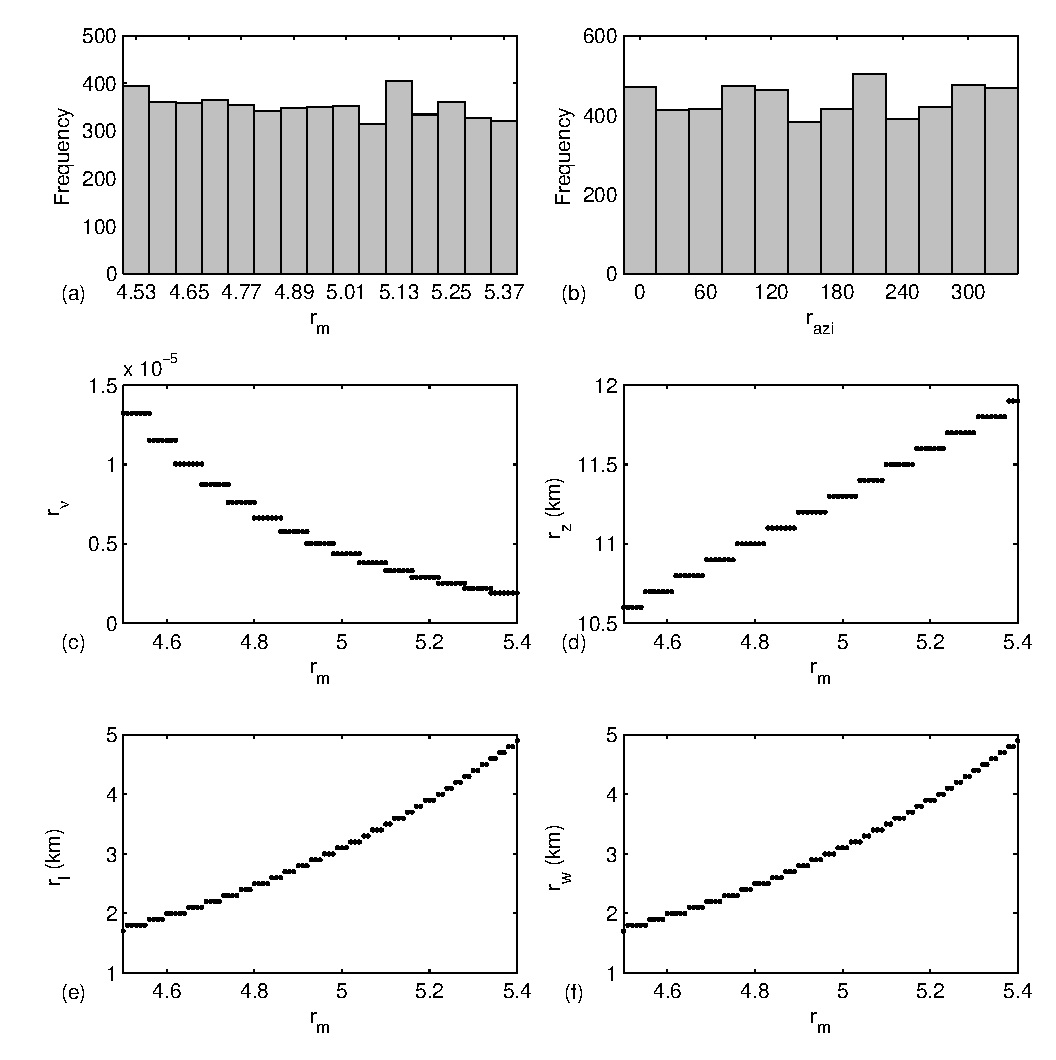
\includegraphics[width=1\textwidth]{fig-hsource-eventstatstri}
\end{center}
\caption{Simulated events for the Newcastle Triangle Zone (see
\citealt{dr_Dhu02b}). Plots (a) and (b) show histograms of the
rupture magnitude $r_m$ and rupture azimuth $r_{azi}$
respectively. Plots (c), (d), (e) and (f) illustrate the
relationship between the event magnitude $r_m$ and the event
activity $r_\nu$, the depth to the rupture centroid $r_z$, the
length of the rupture $r_l$ and the width of the rupture $r_w$
respectively. The desired number of events $ntrgvector(1)$ was
$5000$.} \label{fig:source-catalogue-results1}
\end{figure}

\begin{figure}
\begin{center}
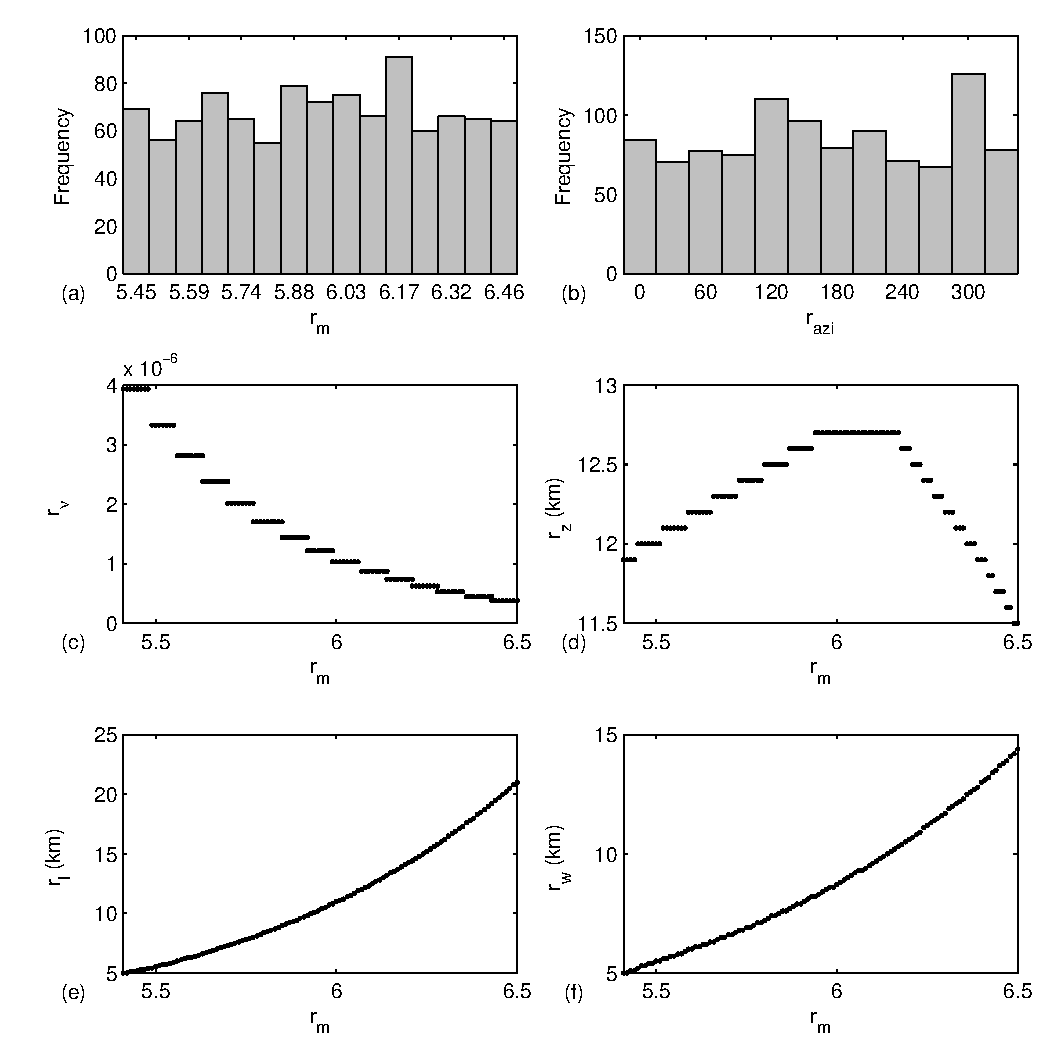
\includegraphics[width=1\textwidth]{fig-hsource-eventstatsrec}
\end{center}
\caption{Simulated events for the Newcastle Rectangle Zone (see
\citealt{dr_Dhu02b}). Parts (a) to (f) are the same as those
described in \fref{fig:source-catalogue-results1}. The desired
number of events $ntrgvector(4)$ was $3000$.}
\label{fig:source-catalogue-results2}
\end{figure}

\begin{figure}
\begin{center}
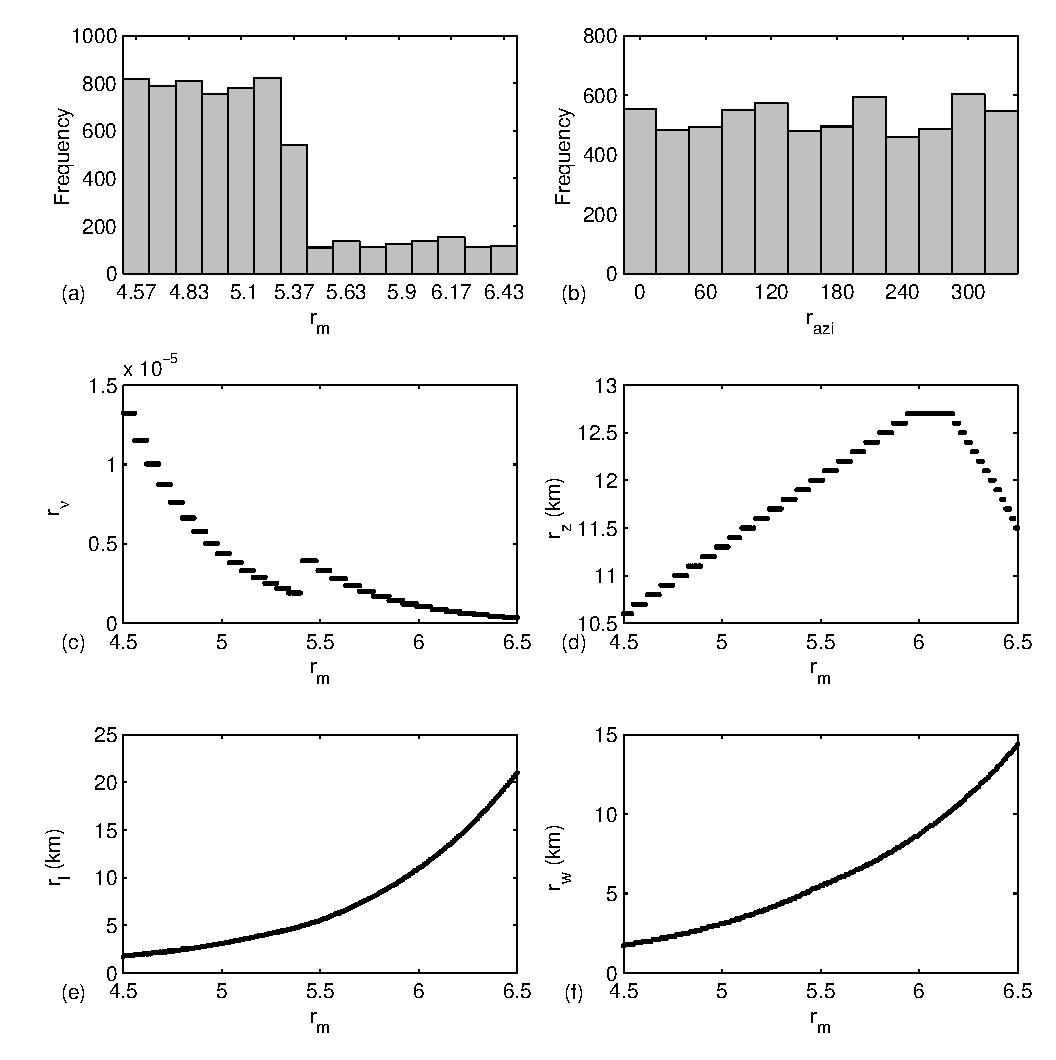
\includegraphics[width=1\textwidth]{fig-hsource-eventstats_tri_rec}
\end{center}
 \caption{Simulated
events when the Newcastle Triangle Zone and Newcastle Fault Zone
are considered together (see \citealt{dr_Dhu02b}). Parts (a) to
(f) are the same as those described in
\fref{fig:source-catalogue-results1}. The desired number of events
was defined by $ntrgvector = [5000,3000]$ where the source zones
$1$ and $2$ refer to the the Newcastle Triangle Zone (NTZ) and the
Newcastle Fault Zone respectively.}
\label{fig:source-catalogue-results3}
\end{figure}



\begin{figure}
\begin{center}
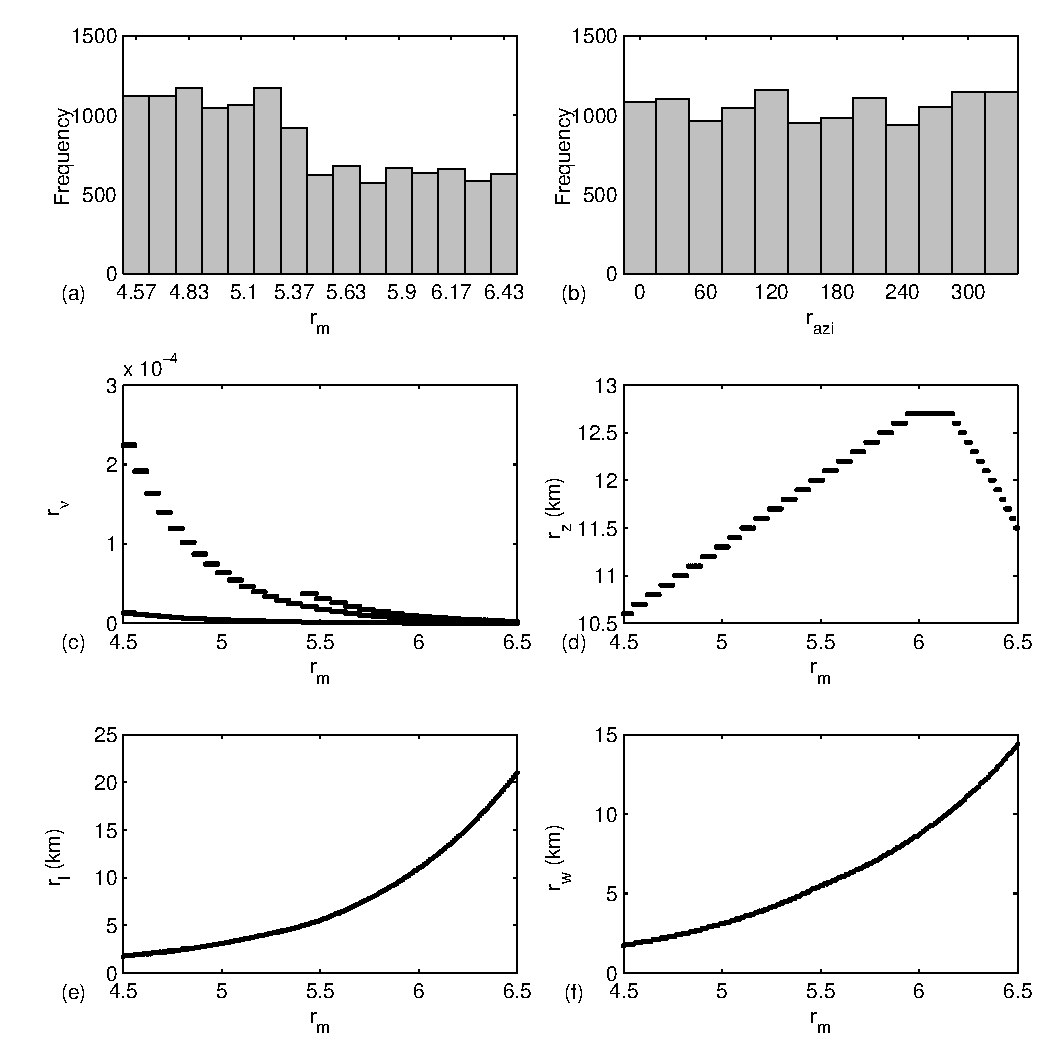
\includegraphics[width=1\textwidth]{fig-hsource-eventstatsall}
\end{center}
\caption{Simulated events for all six of the source zones used in
the Newcastle and Lake Macquarie study (see \citealt{dr_Dhu02b}).
Parts (a) to (f) are the same as those described in
\fref{fig:source-catalogue-results1}. The desired number of events
was defined by $ntrgvector = [5000,1000,1000,3000,1000,1000]$
where the source zones $1$ to $6$ refer to the the Newcastle
Triangle Zone (NTZ) the Tasman Sea Margin Zone Subset 1 (TSMZ1),
the TSMZ2, the Newcastle Fault Zone, the TSMZ3 and the TSMZ4
respectively.} \label{fig:source-catalogue-results4}
\end{figure}


\subsection{Dimensions and position of the rupture plane}
\label{sec:dim-rupture}


The width and length of the rupture and position of the rupture
centroid are computed by \typefunc{mag}{2rup}{\_v} using empirical
rules based on the moment magnitude, $r_m$ of the event (Mendez,
2002 [\textit{pers. comm.}]) . The location of the rupture plane
is constrained to lie within a virtual fault\index{virtual fault}
which is described by the depth to its top (equivalent to the
depth to the seismogenic region $f_z$, see
\sref{tab:site-loc-par-sourcezones}), its length $f_l$, its width
$f_w$ and its dip $r_{dip}$. Note that by default the dip of the
 rupture plane is defined to be the dip of the virtual fault\index{virtual fault}.
Firstly, the area of the rupture plane $A_r$ is defined as
\begin{equation}
A_r = 10^{r_m - 4.02}
\end{equation}
which represents a subtle change from that defined by
\citet*{dr_Wells94a}. Empirical relationships for the width $r_w$
and length $l_r$ of the rupture plane were defined by Mendez (2002
[\textit{pers. comm.}]). The width is defined in a two step
process as follows
\begin{equation}
 f_1 = \left \{ \begin{array}{ll}
 1 & \textrm{if $r_m \leq 5.5$} \\
\frac{1}{\sqrt[\leftroot{-2}\uproot{2}4]{1+2(r_m-5.5)\sin(r_{dip})}} & \textrm{if $r_m>5.5$} \\
\end{array} \right.
\end{equation}

and

\begin{equation}
r_w = \textrm{min$\{f_1\sqrt{A_r},f_w\}$}.
\end{equation}

Recall from \sref{sec:event-catalogue} that the rupture centroid
$(r_x,r_y,r_z)$ is defined in terms of a local coordinate system.
The depth of the rupture centroid is determined in a two step
process as follows:

\begin{equation}
f_2 = \left \{ \begin{array}{ll} 1 & \textrm{if $r_m\leq4$} \\
1 + \frac{r_m-4}{2} & \textrm{if $4<r_m\leq6$} \\
2 & \textrm{if $r_m\geq6$} \\
\end{array} \right.
\end{equation}

and
\begin{equation}
r_z = \textrm{min$\{f_z+\frac{f_2}{3}f_w\sin(r_{dip}),
f_z+f_w\sin(r_{dip})-\frac{1}{2}r_w\sin(r_{dip})\}$}.
\end{equation}

The other two coordinates of the rupture centroid are given by
\begin{equation}
r_y = r_z\cot(r_{dip})
\end{equation}

and

\begin{equation}
r_x = \frac{r_l}{2}.
\end{equation}
The depth to the rupture centroid $r_z$ and the length and width
of the rupture plane are illustrated for four separate simulations
in
\Frefmulti{fig:source-catalogue-results1}{fig:source-catalogue-results4}(d),
(e) and (f) respectively.



\subsection{Azimuth and dip of rupture}
\label{sec:az-dip-rupture}

The rupture azimuth of each event may be forced to lie within a
user defined range
\begin{center} $\phi - d_{\phi} \leq r_\phi \leq \phi + d_{\phi}$ \end{center}
where $\phi$ and $d_{\phi}$ are \typepar{a}{z}{i} and
\typepar{d}{\_a}{zi} in \typeself{set}{da}{ta} respectively. The
default values for $\phi$ and $d_{\phi}$ are $180^o$ and $180^o$
respectively. Recall that the azimuth is further adjusted through
the process described in \sref{sec:rup-location}, unless $d_{azi}$
is assigned to a negative number. Note that in the current version
of the EQRM application this adjustment process ignores the above
azimuth bound. That is, the azimuth of one or more events may be
adjusted outside the above range in an attempt to force the
event's end point to lie within the source zone. The distribution
of simulated azimuth for four different simulations is illustrated
in
\Frefmulti{fig:source-catalogue-results1}{fig:source-catalogue-results4}(b).

The dip of the rupture, $r_{dip}$, is assigned in
\typeself{set}{da}{ta} and may take only a single value for all
source zones. The dip of the rupture trace is measured from the
ground surface and the direction of dip is such that the plane is
located in the region of $y>0$ in the local coordinate system.
Note that it is
 possible to modify the software to select the dip randomly in a similar fashion to that
 described for the azimuth above. However, it is worth noting that
 the effect of a change in dip varies based on the attenuation model (see \sref{ch:atten}). For example, when using an attenuation model that depends on the Joyner-Boore distance, the practical effect
 of a change in dip can be compensated by a
 horizontal translation of the rupture trace. In such cases the random
 location of the rupture trace negates the need to select the dip
 randomly.

\section{Using multiple source zones - Incorporating epistemic uncertainty}
\label{sec:source-multizones}

Recall that \sref{sec:source-EQcat} introduced two techniques for
passing source models to the EQRM:
\begin{enumerate}
\item the
\typeparfilecaption{<site\_loc>}{\_par}{\_sourcezones}{.txt} and
\typeparfile{<site\_loc>}{\_par\_sou}{rcepolys}{.txt} file pair,
and \item the
\typeparfilecaption{<site\_loc>}{\_par}{\_source}{.mat} file.
\end{enumerate}
Recall also that the notion of a `generation
polygon'\index{generation polygon} was introduced where the
generation polygons are simply the individual source zones when
Technique 1 is used, and `generation polygon' refers to the
polygons in the \typevar{gen}{erat}{ion} variable when Technique 2
is used. This definition ensured that the discussion of earthquake
location (\sref{sec:rup-location}), rupture geometry
(\sref{sec:dim-rupture}), azimuth and dip
(\sref{sec:az-dip-rupture}) described above is applicable to both
of the two techniques for providing source information to the
EQRM. When Technique 2 is used, however, a minor modification must
be made to the algorithm described for magnitude and event
activity determination (see \sref{sec:magnitude_selection}). To
explain the differences in the algorithm and to explain the
incorporation of multiple source zone models (epistemic
uncertainty with source models) the reader will need to understand
the contents of the
\typeparfile{<site\_loc>}{\_par}{\_source}{.mat} file.

The \typeparfile{<site\_loc>}{\_par}{\_source}{.mat} file contains
the following two variables:
\begin{enumerate}
\item The \typevar{gen}{erat}{ion} variable is a MATLAB structure
containing the fields \texttt{zones} and \texttt{polys}. The field
\texttt{zones} is a matrix containing the same format as that
described in \tref{tab:site-loc-par-sourcezones}. The number of
rows refers to the number of `generation polygons' to be used in
the generation process. It is common to have 2 `generation
polygons' arranged in a doughnut shape with an inner and outer
polygon. The inner polygon is typically centered on the region of
interest and can be used to simulate a larger number of
earthquakes (hence higher spatial concentration) than the outer
polygon. The field \texttt{polys} is a matrix using the same
format as \tref{tab:site-loc-par-sourcepolys} to describe the
vertices of the polygons in the field \texttt{zones}. \item The
\typevar{sou}{rc}{e} variable is a MATLAB structure array
containing one element for each source zone model to be used. The
number of elements in the \typevar{sou}{rc}{e} structure array
corresponds to the number of source zone models to be used in the
simulation. Each element has fields \texttt{zones}, \texttt{polys}
and \texttt{weight}. The fields \texttt{zones} and \texttt{polys}
are similar to those described in 1 above, however this time they
represent the individual source source zones for the source model.
The field \texttt{weight} represents the weight to be applied to
the source zone model.
\end{enumerate}

When using Technique 2 the \typevar{gen}{er}{ation} is used to
define the `generation polygons' and hence the location, geometry,
azimuth and dip of the rupture. The variable
\typevar{gen}{er}{ation} is also used to assign magnitudes to each
synthetic event\index{synthetic event} using Steps 1 to 4 from
\sref{sec:magnitude_selection}. Note that a synthetic earthquake
generated in this fashion may lie in none, one or multiple source
zones from the different source models. The calculation of an
event activity involves identifying which zones the earthquake
lies within and then computing the weighted sum of individual
event activities for the zones within which it lies. The algorithm
for computing the event activity for a single source zone is
described in Step 5 of \sref{sec:magnitude_selection}. Note that
an earthquake must fall within the polygon that defines the source
zone and its magnitude must be within the magnitude bounds for the
source zone before it is considered to lie within the source zone.
More details of this process can be found by looking at the
functions \typefunc{calc}{\_event}{\_activity} for the calculation
of event activity and \typefunc{mke}{\_aseq}{4mat} for all of
processes.

\section{Spawning events}
\label{source:spawning}


There is an option within the EQRM application to spawn (or copy)
events. Such copies are required by some techniques for
incorporating aleatory uncertainty in later stages of the PSHA and
PSRA. For example, \sref{attn:uncert-randomchoice} describes an
incorporation of aleatory attenuation uncertainty that does not
require spawning of the catalogue whereas
\sref{attn:uncert-pdfchoice} describes a process that does require
spawning.  The option is performed by \typefunc{fuse}{\_4}{hzd}.
Actually \typefunc{fuse}{\_4}{hzd} is an essential component of
any earthquake hazard or risk run with the
\typeselfnoindex{}{}{EQRM} application i.e. it must be run
regardless of whether the user wishes to spawn events or not. The
spawning of events is controlled by \typepar{src}{\_eps}{\_switch}
in \typeself{set}{da}{ta}. If
\mbox{\typepar{src}{\_eps}{\_switch}$ = 1$ or $-1$} then all
events with magnitude greater than $m_{bnd}$ (\typepar{m}{bn}{d}
in \typeself{set}{da}{ta}) are copied $n_{samples}$
(\typepar{nsa}{mpl}{es} in \typeself{set}{da}{ta}) times with
their event activity adjusted according to a weight $w_e$. If
\mbox{\typepar{src}{\_eps}{\_switch}$ = 0$} no spawning is
undertaken. When spawning the weight $w_e$ is derived by
truncating and re-normalising a standard normal distribution to
$\pm n_\sigma$ (\typepar{n}{sig}{ma} in \typeself{set}{da}{ta}).
The process is summarised below.

We know that the standard normal distribution $ N \sim (0,1)$ has
a PDF given by
\begin{equation}
\begin{array}{lr}
f_X(x)=\frac{1}{\sqrt{2\pi}}e^{\frac{-x^2}{2}} & - \infty <x<
\infty.
\\
\end{array}
\end{equation}

To truncate and re-normalise $N \sim (0,1)$ to $\pm n_\sigma$ we
must evaluate $P(-n_\sigma \sigma \leq X \leq n_\sigma \sigma)$.
The error function
\begin{equation}
erf(x) = \frac{2}{\sqrt{\pi}} \int_{0}^{x} e^{-t^2} \, dt.
\end{equation}
is related to the cumulative area under the standard normal
distribution via
\begin{equation}
erf(x) = 2P(X \leq x)-1.
\end{equation}
The function \typefunc{mke}{\_ct}{pdf} computes $P(-n_\sigma
\sigma \leq X \leq n_\sigma \sigma)$ using the error function as
follows
\begin{equation}
\begin{array}{rcl}
P(-n_\sigma \sigma \leq X \leq n_\sigma\ \sigma)  & = & P(X \leq
n_\sigma)-P(X \leq -n_\sigma) \\
   & = & 2P(X \leq n_\sigma)-1 \\
    & = & erf(n_\sigma) . \\
\end{array}
\end{equation}

Then, \typefunc{mke}{\_ct}{pdf} computes the truncated and
re-normalised PDF by evaluating
\begin{equation}
\begin{array}{lr}
\tilde{f}_X(x)= \frac{1}{P(-n_\sigma \sigma \leq X \leq n_\sigma
\sigma)}
\frac{1}{\sqrt{2\pi}}e^{ \frac{-x^2}{2}} & -n_\sigma \sigma <x< n_\sigma \sigma. \\
\end{array}
\end{equation}

The observant reader will notice that because the EQRM application
works in the discrete world, simply evaluating $\tilde{f}_X(x)$
will not suffice. The approach used by \typefunc{mke}{\_ct}{pdf}
to discretise $\tilde{f}_X$ and compute the weights
$\{w_{e,i}\}_{i=1}^{n_{samples}}$ is identical to that used to
compute the event activity $r_\nu$ (see
\sref{sec:magnitude_selection}) and is described in
\aref{app:discret-pdf}. That is
\begin{equation}
w_{e,i} = \frac{\tilde{f}_X(x_i)}{\sum\limits_{j=1}^{n_{samples}}
\tilde{f}_X(x_j)}.
\end{equation}
Once the weights $\{w_{e,i}\}_{i=1}^{n_{samples}}$ are computed
the event activity $r_\nu$ for each of the event copies is
re-defined as follows:
\begin{equation}
\label{source:spawning-activity}
\begin{array}{ll}
r_{\nu,i} = r_{\nu,original} \times w_{e,i} & \textrm{for } i=1
\textrm{ to } n_{samples},
\end{array}
\end{equation}
for each copy of the original event and its associated weighting.
A source epsilon term $r_\varepsilon$ is also defined for each
copy of the original event i.e.
$\{r_{\varepsilon,i}\}_{i=1}^{n_{samples}}$. Each of the
$r_{\varepsilon,i}$ are defined such that they correspond to the
$i^{th}$ bin centroid from the $n_{samples}$ bin spanning $\pm
n_\sigma$ (see \sref{attn:uncert-pdfchoice} for the mathematical
definition).


\section{Analysing a scenario event}
\label{sec:source-scenario} The EQRM application (through
\typefunc{mke}{\_ev}{nts}) incorporates an option for considering
a particular (or scenario) event. This option is instigated when
the user defines \typepar{det}{erm}{\_flag}$=1$ in
\typeself{set}{da}{ta}. The earthquake catalogue takes the same
form as that described in \tref{tab:evntdb-columns}. The scenario
event is constrained by user defined values for magnitude
(\typepar{det}{erm}{\_mag}), position
(\typeparcaption{det}{erm}{\_lat} and \typepar{det}{erm}{\_lon}),
depth (\typeparcaption{det}{erm}{\_r\_z}) and azimuth
(\typepar{det}{erm}{\_azi}).

\newpage
\section{Key functions, flags and parameters}

\begin{tabular}{llp{0.55\textwidth}}
\hline
\textbf{Name} & \textbf{Type} & \textbf{Description} \\
\hline
\keyrowsep \typefunc{mke}{\_ev}{nts} & Function & Master file for creating an event catalogue.\\
\keyrowsep \typefunc{mke}{\_aseq}{4mat} & Function & Handles a significant proportion of the synthetic event generation on behalf of \typefunc{mke}{\_ev}{nts}. \\
\keyrowsep \typefunc{m2}{gr}{pdfb} & Function & Computes the PDF, $f_M$ for the bounded Gutenberg-Richter distribution. \\
\keyrowsep \typefunc{mag}{2rup}{\_v} & Function & Computes rupture dimension and `relative' location based on magnitude. \\
\keyrowsep \typefunc{fuse}{\_4}{hzd} & Function & Master file for spawning events. \\
\keyrowsep \typefunc{mke}{\_ct}{pdf} & Function & Truncates and discretises $N\sim(0,1)$. \\
\keyrowsep \typepar{a}{z}{i} & Par & Centre of azimuth range for events. \\
\keyrowsep \typepar{d}{\_a}{zi} & Par & Half width of azimuth range. \\
\keyrowsep \typepar{d}{i}{p} & Par & Dip of virtual fault\index{virtual fault}. \\
\keyrowsep \typepar{ntrg}{vec}{tor} & Par & Vector whose elements represent the desired number of events to be simulated in each source zone. \\
\keyrowsep \typepar{w}{d}{th} & Par & Width of virtual fault\index{virtual fault}. \\
\keyrowsep \typepar{n}{bin}{s} & Par & Number of bins for event magnitude sampling. \\
\keyrowsep \typepar{src}{\_eps}{\_switch} & Par &  Events are (not) spawned if \typepar{src}{\_eps}{\_switch} $= 1$ ($=0$). \\
\keyrowsep \typepar{m}{bn}{d} & Par &  Only events with magnitude greater than \typepar{m}{bn}{d} are spawned. \\
\keyrowsep \typepar{nsa}{mpl}{es} & Par & Creates \typepar{nsa}{mpl}{es} copies of each spawned event. \\
\keyrowsep \typepar{n}{sig}{ma} & Par &  Range of distribution to be considered when spawning. \\
\keyrowsep \typepar{det}{erm}{\_flag} & Par & EQRM application used in scenario mode if \typepar{det}{erm}{\_flag} $=1$. \\
\keyrowsep \typepar{det}{erm}{\_mag} & Par & Magnitude of scenario event. \\
\end{tabular}


\begin{tabular}{llp{0.55\textwidth}}
\keyrowsep \typepar{det}{erm}{\_lat} & Par & Latitude of scenario epicenter (corresponds to $r_c^{lat}$). \\
\keyrowsep \typepar{det}{erm}{\_lon} & Par &  Longitude of scenario epicenter (corresponds to $r_c^{lon}$). \\
\keyrowsep \typepar{det}{erm}{\_r\_z} & Par &  Depth to scenario epicenter in $km$ (corresponds to $r_z$). \\
\keyrowsep \typepar{det}{erm}{\_azi} & Par &  Azimuth of scenario event (corresponds to $r_\phi$). \\
\hline
\end{tabular}






%%% Local Variables:
%%% mode: latex
%%% TeX-master: "eqrmtech"
%%% End:

\chapter{Ground-Motion Prediction Equations}
\label{ch:atten}

\newcommand{\Rhyp}{R_{\mathrm{hyp}}}
\newcommand{\Repi}{R_{\mathrm{epi}}}
\newcommand{\Rrup}{R_{\mathrm{rup}}}
\newcommand{\Rjb}{R_{\mathrm{jb}}}

\section{Overview}

Ground-Motion Prediction Equations (GMPEs) play key role in the
evaluation of seismic hazard in the region of interest. In this
chapter, we mainly focus on how EQRM deals with GMPEs and
corresponding uncertainties. However, to help the interested user to
become more familiar with the state-of-art and issues on using GMPEs
in the framework of seismic hazard analysis, each section comes with
a set of useful references. The remainder of this chapter is
organised as follows. First, the background theory of GMPEs is
addressed in ~\sref{sec:background}. Then, an introduction on the
selected GMPEs is brought in ~\sref{sec:implemented}.
~\sref{sec:implementation} describes how the selected GMPEs are
implemented in EQRM. Finally, capturing of uncertainties in EQRM,
which is a major challenge in estimation of strong motions, forms
the last section of this chapter.


\section{Background theory} \label{sec:background} The
Ground-Motion Prediction Equations (GMPEs), also referred to as
attenuation models, are used to describe the attenuation of the
ground-motion parameter of interest with respect to parameters of
the earthquake source, propagation path and local site conditions,
collectively referred to as seismological parameters. These
equations are obtained from regression analysis on the recorded or
synthetic values of the parameter of interest. A GMPE can be
described by the general expression as:
\begin{equation}\label{eq:general}
\ln Y =f(x,\theta)+\varepsilon,
\end{equation}
where $Y$ is the median of the ground-motion parameter of interest,
$x$ is the vector of seismological parameters, $\theta$ is the
vector of the GMPE’s regression coefficients, and $\varepsilon$ is
a random error term with a mean of zero and a standard deviation of
$\sigma_{\ln Y}$ . In this regard, for a given set of seismological
parameters, a GMPE describes the probability density function (PDF)
of the ground-motion parameter as a lognormal distribution with
median and standard deviation equal to $Y$, and  $\sigma_{\ln Y}$,
respectively ($f(Y|x)$). This is a basic requirement by seismic
hazard analysis (SHA) in order to calculate the probability of
exceeding desired ground-motion level for a given set of
seismological parameters.

In engineering practice, traditionally, the most desired
ground-motion parameters are Peak Ground Velocity (PGV), Peak Ground
Acceleration (PGA), and $5\%$ damped Pseudo Spectral Acceleration
(PSA or SA)of horizontal components. There are a number of ways to
define the response variable based on two horizontal components,
such as considering the perpendicular horizontal components to be
independent, and geometric mean of horizontal components. Although
using the geometric mean has the advantage that the standard
deviation for the ground-motion models is smaller than for other
measures (Beyer and Bommer 2006), this measurement nevertheless
depends on the orientations of the sensors installed in the field.
Recently, alternative definitions of ground motion that are
independent of the sensor orientation was introduced by Boore et al.
(2006). These parameters, so called as GMRotI50, and GMRotD50 are
based on a set of geometric means computed from the recorded
orthogonal horizontal motions after rotating them through a
non-redundant angle of 90.

The most widely used seismological parameters by GMPEs are
earthquake magnitude (source parameter), source-to-site distance
measure (path parameter), and description of local site condition
(site parameter).

The earthquake magnitude is used to measure the size of the
earthquake. There are different scales to define magnitude. The most
commonly magnitude scales that are used in the development of the
GMPEs throughout the world are moment magnitude, $M_W$ and surface
wave magnitude, $M_S$. However, many GMPEs use local magnitude
scale, $M_L$, for smaller magnitude earthquakes. The $M_W$ scale has
been used by most of the recent GMPEs. It is based on the moment of
the earthquake ($M_0$), which is a measure of the seismic energy
radiated by an earthquake:
\begin{equation}\label{eq:MW}
M_W=\frac{2}{3}\log {M_0}-10.7.
\end{equation}
The main advantages of $M_W$ scale are that it is not saturated at
the upper end and it can be determined from geological faulting
measurements or from seismic waves.

Source-to-site distance measure is used to characterise the
attenuation of the ground motion amplitude versus distance from the
earthquake source. Different measures of distance are used by
different GMPEs. These measures are illustrated in
\Fref{fig:attn-distances} and can be summarized as follows:

Point-source distance measures:
\begin{itemize}
\item Hypocentral distance ($R_{hypo}$): Distance from the hypocenter of an earthquake to the site of interest.
\item Epicentral distance ($R_{epi}$): Distance from the epicenter of an earthquake to the site of interest.
\end{itemize}

Finite-source distance measures:
\begin{itemize}
\item Fault distance ($R_{rup}$): Closest distance between rupture plane and site of interest.
\item Joyner-Boore distance ($R_{jb}$): Closest distance between surface projection of the rupture plane and site of the interest.
\item Seismogenic distance ($R_{seis}$): Closest distance between seismogenic part of the rupture plane and site of the interest.
\end{itemize}
\begin{figure}[htp]
 \centering \psfrag{Rjb}{$\Rjb$}
\psfrag{Rhyp}{$\Rhyp$} \psfrag{Rrup}{$\Rrup$} \psfrag{Repi}{$\Repi$}
\psfrag{site}{site} \psfrag{fault}{fault} \psfrag{d}{$h$}
\includegraphics[width=0.7\textwidth]{diags/fig-hattn-distance}
\caption{Diagram showing the distance measures used in various
  attenuation formulae.}
  \label{fig:attn-distances}
\end{figure}
In case of small earthquake that can be represented by a point
source, the point source measures can be considered as
source-to-site distance measure. However, the point source measures
are not suitable to describe the attenuation of ground motion away
from large earthquakes. In this case, the finite source measures are
preferred.

Local site conditions profoundly affect the ground motion record
characteristics. Several numerical and/or empirical techniques have
been proposed to estimate local site responses. Such studies show
distinct amplification levels in the sites of different geological
and geotechnical characteristics; therefore, it is an ordinary
practice to categorize sites into different general classes.
Different sites of the same class are supposed to have local site
responses with similar main characteristics. The most commonly used
site categorization schemes by GMPEs are based on geomatrix, surface
geology, and average shear wave velocity over 30m ($V_{S30}$).
Actually, many of the GMPEs follow exactly the same or similar
classification criteria as suggested by NEHRP (Table ~\ref{NEHRP}).
$V_{S30}$ has also been included directly in the functional form of
several attenuation models. It is worth mentioning that in spite of
$V_{S30}$ popularity as a site parameter, it has its own
shortcomings. Several studies have suggested using other site
parameters such as the average shear wave velocity over the depth
equal to a quarter-wavelength of the period of interest, and the
average shear wave velocity of 100-200m.
\begin{table}[!t]
\renewcommand{\arraystretch}{1.3}
\caption{Site categories in NEHRP provisions} \label{NEHRP}
\centering
\begin{tabular}{|c|c|c|}
\hline
Site Category & Description & $V_{S30}$\\
\hline
A & Hard rock & $>1500 m/s$\\
\hline
B & Firm to hard rock & $760-1500 m/s$\\
\hline
C & Dense soil, soft rock & $360-760 m/s$\\
\hline
D & Stiff soil & $180-360 m/s$\\
\hline
E & Soft clays & $<180 m/s$\\
\hline
\end{tabular}
\end{table}

\section{Implemented GMPEs in EQRM}\label{sec:implemented} In
recent years the number of GMPEs is considerably increased due to
development of strong motion networks and the large number of
available strong motion records. Douglas (2003) provides a review on
more than 120 GMPEs for the estimation of peak ground acceleration
and 80 GMPEs for the estimation of response spectra. Generally,
GMPEs can be grouped into two different principle tectonic regions:
shallow crustal earthquakes and subduction zone earthquakes. The
shallow crustal earthquakes can be further divided into earthquakes
in active tectonic regions (e.g. Japan, California, Iran), and
earthquakes in stable continental regions (e.g. Australia, Eastern
North America). The subduction zone earthquakes can be further
divided into intraslab events and earthquakes along the interface of
subducting plates (e.g. Japan, Chile, Indonesia). For details of the
main characteristics of each category see Campbell (2003). For each
tectonic region, a handful of GMPEs are available for use within
EQRM software. Their main characteristics are summarized in
Table~\ref{GMPEs}. All of these equations are widely used in
engineering and engineering seismology. They reflect a broad variety
of tastes in terms of their functional forms and databases.
\begin{landscape}
\begin{table}[!t]
\renewcommand{\arraystretch}{1.3}
\caption{Main characteristics of the implemented GMPEs}
\label{GMPEs} \centering
\begin{tabular}{|c|c|c|c|c|c|c|c|c|}
\hline {\footnotesize Model} & {\footnotesize Magnitude} &
{\footnotesize Magnitude} & {\footnotesize Distance} &
{\footnotesize Distance} & {\footnotesize Site}
& {\footnotesize Horizontal Component} & {\footnotesize Period} & {\footnotesize Complexity}  \\
{\footnotesize Name} & {\footnotesize Type} & {\footnotesize Range}
& {\footnotesize Type} & {\footnotesize Range} & {\footnotesize
Condition}
& {\footnotesize Type} & {\footnotesize Range} &\\
\hline \multicolumn{9}{|c|}{Shallow crustal events in active
tectonic regions}\\
\hline {\footnotesize Sadigh et al. (1997)} & $M_W$ & 4-7.4 &
$R_{rup}$ &
0-100& $GMX$ & Geometric mean & 0-4 & 9\\
\hline {\footnotesize Zhao et al. (2006)} & $M_W$ & 4.9-8.3 &
$R_{rup}$ &
0-300& $V_{S30} Class$ & Geometric mean & 0-5 & 16\\
\hline {\footnotesize Abrahamson and Silva (2008)} & $M_W$ & 5.0-8.0
&
$R_{jb}$ & 0-200 & $V_{S30}$ & GMRotI50 & 0-10 & 17\\
\hline {\footnotesize Boore and Atkinson (2008)} & $M_W$ & 5.0-8.0 &
$R_{rup}$ & 0-200 & $V_{S30}$ & GMRotI50 & 0-10 & 14\\
\hline {\footnotesize Campbell and Bozorgnia (2008)} & $M_W$ &
4.0-8.5 &
$R_{rup}$ & 0-200 & $V_{S30}$ & GMRotI50 & 0-10 & 17\\
\hline {\footnotesize Chiou and Youngs (2008)} & $M_W$ & 4.0-8.5 &
$R_{rup}$ & 0-200 & $V_{S30}$ & GMRotI50 & 0-10 & 25\\
\hline {\footnotesize Akkar and Bommer (2010)} & $M_W$ & 5.0-7.6 &
$R_{jb}$
& 0-100& $V_{S30}$ Class & Geometric mean & 0-3 & 14\\
\hline \multicolumn{9}{|c|}{Shallow crustal events in stable
continental regions}\\
\hline {\footnotesize Gaull et al. (1990)} & $M_L$ & ?  &
$R_{hypo}$& 10-500& $V_{S30}$ Class & Random & 0-2 & ?\\
\hline {\footnotesize Atkinson and Boore (1997)} & $M_W$ & 4.0-7.25
&
$R_{hypo}$& 10-500& $V_{S30}$ Class & Random & 0-2 & 5\\
\hline {\footnotesize Toro et al. (1997)} & $M_W$ & 5.0-8.0 &
$R_{jb}$& 1-500& Hard Rock & Geometric mean & 0-2 & 9\\
\hline {\footnotesize Campbell (2003)} & $M_W$ & 5.0-8.2 &
$R_{rup}$& 1-1000& Hard Rock & Geometric mean & 0-4 & 13\\
\hline {\footnotesize Atkinson and Boore (2006)} & $M_W$ & 4.0-8.0 &
$R_{rup}$& 1-1000& $V_{S30}$ & Random & 0-5 & 14 \\
\hline {\footnotesize Liang et al. (2008)} & $M_L$ & 4.0-7.0 &
$R_{epi}$& 10-200& Hard Rock & Random & 0-30 & 6\\
\hline {\footnotesize Somerville (2009)} & $M_W$ &5-7.5  &
$R_{jb}$& 0-500& Hard Rock &  ?& 0-10 & 10\\

\hline \multicolumn{9}{|c|}{Subduction zone events}\\
\hline {\footnotesize Youngs et al. (1997)} & $M_W$ & 5.0-8.2 &
$R_{rup}$& 10-500& GMX & Geometric mean & 0-3 & 7\\
\hline {\footnotesize Atkinson and Boore (2003)} & $M_W$ & 5.0-8.3 &
$R_{rup}$& 10-500& $V_{S30}$ Class & Random & 0-3 & 9\\
\hline {\footnotesize Zhao et al. (2006)} & $M_W$ & 5.0-8.3 &
$R_{rup}$ &
30-300& $V_{S30} Class$ & Geometric mean & 0-5 & 16\\
\hline

\end{tabular}
\end{table}
\end{landscape}

Considering the general tectonic setting of the region of interest,
the user may either select GMPEs from those listed in
Table~\ref{GMPEs}, or implement his or her desirable model. It
should be also noted that GMPEs have to be selected based on their
magnitude and frequency validity ranges. In other words, GMPEs
should not be used outside the ranges of their underlying dataset
(Bommer et al., 2007). General guidelines on selection of GMPEs for
seismic hazard analysis are provided by Cotton et al. (2006) and
Bommer et al. (2010). In addition, if strong motion data is
available in the target region, it can be used to verify candidate
GMPEs. To compare ground motions or GMPEs between regions, the main
approaches are the direct comparison of median predictions from
GMPEs for different regions (Campbell and Bozorgnia, 2006; Stafford
et al., 2008), analysis of variance (Douglas, 2004a, b), and
evaluation of the consistency of data distributions with respect to
a GMPE using likelihood concepts (Scherbaum et al., 2004; Stafford
et al., 2008) or information-theory approach (Scherbaum et al.,
2009).

The complexity of the implemented GMPEs varies based on the database
size and developers preferences. In Table~\ref{GMPEs}, the
complexity of each GMPE is represented as the number of the
regression coefficients. In addition to magnitude scaling, distance
scaling and local site condition terms, some of the GMPEs have extra
terms to model other phenomena affecting the ground motion
amplitudes. Table ~\ref{terms} lists such terms for GMPEs developed
for active crustal regions. As it can be seen, among the selected
GMPEs, Abrahamson and Silve (2008), Campbell and Bozorgnia (2008),
and Chiou and Youngs (2008) models can be considered as the most
complex ones with many input parameters required. They notably
require extra input parameters to model: (1) observed higher
ground-motions on the hanging-wall of the fault-plane, (2) larger
ground-motions generated by buried rupture earthquakes, and (3)
basin effect which is believed to have significant impact on
amplification of ground motion especially at longer period range.
The mentioned GMPEs as well as Boore and Atkinson (2008) model
account for nonlinear site amplification that is due to nonlinear
soil response beyond a certain level of deformations. These models
are developed as part of the Next Generation of Attenuation of
Ground-Motions (NGA) project in 2008 for shallow crustal earthquakes
in California. In many regions, however, it is not possible to
determine all the necessary input parameters for such complicated
models. General guidelines on estimating unknown input parameters
when implementing NGA GMPEs in engineering practice are presented in
Kaklamanos et al. (2010). The details on how EQRM feeds each of the
implemented GMPEs are given in the next section.
%\begin{landscape}
\begin{table}[!t]
\renewcommand{\arraystretch}{1.3}
\caption{Functional forms of GMPEs for active tectonic regions}
\label{terms} \centering
\begin{tabular}{l l c c c c c c}
\hline
&\multicolumn{7}{|c|}{Ground Motion Prediction Equations}\\
\hline
 Term & {\footnotesize Sa97}& {\footnotesize Zh06
}&{\footnotesize AS08}&{\footnotesize BA08}&
{\footnotesize CB08}&{\footnotesize CY08}& {\footnotesize AB10}\\
\hline {\footnotesize Near-fault} & \textbullet & \textbullet&
\textbullet& \textbullet& \textbullet&
\textbullet&\textbullet\\

{\footnotesize Saturation} \\

\hline {\footnotesize Magnitude-dependent} & & & \textbullet&
\textbullet& \textbullet&
\textbullet& \textbullet\\
{\footnotesize Distance Decay} \\


\hline {\footnotesize Style of Faulting} & \textbullet& \textbullet&
\textbullet& \textbullet& \textbullet& \textbullet& \textbullet\\

\hline {\footnotesize Depth-to-Top } & & & \textbullet& &
\textbullet& \textbullet& \\

{\footnotesize of Rupture}\\

\hline {\footnotesize Hanging-Wall} & & & \textbullet& &
\textbullet& \textbullet& \\

\hline {\footnotesize Basin Effect} & & & \textbullet& &
\textbullet& \textbullet& \\

\hline {\footnotesize Nonlinear } & & & \textbullet& \textbullet&
\textbullet& \textbullet&\\
{\footnotesize Site Response}\\
\end{tabular}
\end{table}
%\end{landscape}
\section{Implementation}\label{sec:implementation} In the EQRM
application the attenuation calculations are conducted within the
main driving function \typefunc{do}{\_ana}{lysis} which computes the
attenuation for one site at a time for all events and all
fundamental (or building) periods. That is, for each site there
exists a large matrix of modelled $S_a(T_o,r_m,R)$ (this matrix is
\typevar{S}{}{A} or \typevar{SA}{ro}{ck} in the code) whose rows
correspond to the events (i.e. an $r_m$-$R$ pair) and whose columns
correspond to the $T_o$. That is

\begin{math}
%\label{fig:attn-sa-matrix}
 SA = \left[ \begin{array}{ccccc}
S_a(T_{o,1},r_{m,1},R_1) & S_a(T_{o,2},r_{m,1},R_1) &  \hdots & S_a(T_{o,N_T},r_{m,1},R_1) \\
S_a(T_{o,1},r_{m,2},R_2) & S_a(T_{o,2},r_{m,2},R_2) &  \hdots & S_a(T_{o,N_T},r_{m,2},R_2) \\
\vdots & \vdots &  \ddots & \vdots \\
S_a(T_{o,1},r_{m,N_s},R_{N_s}) & S_a(T_{o,2},r_{m,N_s},R_{N_s}) & \hdots & S_a(T_{o,N_T},r_{m,N_s},R_{N_s}) \\
\end{array} \right]
\end{math}

where $N_s$ refers to the number of events and $N_T$ refers to the
number of periods. Note that the $r_m$-$R$ pair comes from the event
catalogue and a calculation of distance, as described in this
section. The $T_o$ are determined by the user-defined vector
parameter \typepar{per}{io}{ds} in \typeself{set}{da}{ta}.
Computationally the above calculation of attenuation is conducted in
two parts as follows:
\begin{enumerate}
\item The preparation of the attenuation coefficients
(\typefunc{prep}{\_at}{tn}) conducted before entering a loop over
sites. This preparation involves interpolating the attenuation
coefficients to the fundamental periods defined by
\typepar{per}{io}{ds}. \item The computation of the $S_a(T_o,r_m,R)$
at each site (\typefunc{do}{\_atten}{uation}) conducted site-by-site
within a loop over sites.
\end{enumerate}


Each attenuation model returns an estimate of:
\begin{enumerate}
\item the mean of $log(S_a(T_o,r_m,R))$ (equivalent to the
logarithm of the median of $S_a(T_o,r_m,R)$) and hereafter denoted
by $\mu_{log(S_a)}(T_o,r_m,R)$ or $\mu_{log(S_a)}$ for brevity, and
\item the standard deviation of $log(S_a(T_o,r_m,R))$, hereafter
denoted by \newline $\sigma_{log(S_a)}(T_o,r_m,R)$ or
$\sigma_{log(S_a)}$ for brevity.
\end{enumerate}


The required input parameters by implemented GMPEs in EQRM, to model
source, path and site effects are listed in Table ~\ref{inputs}. The
abbreviations used in this Table are defined in Table ~\ref{def}. As
it can be seen GMPEs use different definitions for explanatory and
response variables. Regarding response parameter,i. e. ground-motion
parameter of interest, currently EQRM estimates $5 \%$ $S_a$ using
GMPEs listed in Table \ref{GMPEs}. The conversion equations between
different definitions of response variables are provided by Beyer
and Bommer (2006).  For each GMPE, EQRM should provide inputs
respecting the original definition used within each model. In EQRM,
the recurrence relationship and hence the generated earthquake
catalogue are based on moment magnitude scale. However, among the
implemented GMPES Gaul et al. (1990), and Liang et al. (2008) models
use $M_L$ scale. In this case, adjustment is done using the
correlation relationship between and as suggested by Johnston
(2001):
\begin{equation}
M_L =
\frac{0.473+\sqrt{0.473^2-4\times0.145(3.45-M_W)}}{2\times0.145};
\end{equation}
Equation 2 is developed for stable continental regions and is based
on earlier work published by the same author (Johnston, 1996). It is
important to note that uncertainties in the explanatory variables
are map to the response variable. In other words, in equation
~\ref{eq:general} if an explanatory parameter, $x$, has been
assigned using a correlation conversion with associated measure of
aleatory variability, $\sigma_x$, then this should be map into the
aleatory variability of the GMPEs, $\sigma_y$, by using the
expression:
\begin{equation}
\sigma_{Total} = \sqrt{\sigma_y^2+(\dfrac{\partial log(Y)}{\partial
x})^2 \sigma_x^2}
\end{equation}
\begin{landscape}
\begin{table}[!t]
\renewcommand{\arraystretch}{1.3}
\caption{Input parameters of the implemented GMPEs in EQRM}
\label{inputs} \centering
\begin{tabular}{c c c c c c c c c c c c c c c c c c}
\hline
&\multicolumn{17}{|c|}{Ground Motion Prediction Equations}\\
\hline
 {\footnotesize Parameter} & {\footnotesize Sa97}& {\footnotesize Zh06}&{\footnotesize AS08}
 &{\footnotesize BA08}&{\footnotesize CB08}&{\footnotesize CY08}&{\footnotesize AB10}&
 {\footnotesize Ga90}& {\footnotesize AB97} &{\footnotesize To97}&
 {\footnotesize Ca03}&{\footnotesize AB06}&{\footnotesize Li08}&{\footnotesize So09}
 &{\footnotesize Yo97}&{\footnotesize AB03}&{\footnotesize Zh06}\\
\hline {\footnotesize Source parameters}\\
$M_L$&&&&&&&&\textbullet&&&&&\textbullet&&&&\\
$M_W$&\textbullet&\textbullet&\textbullet&\textbullet&\textbullet&\textbullet&\textbullet
&&\textbullet&\textbullet&\textbullet&\textbullet&&\textbullet&\textbullet
&\textbullet&\textbullet\\
$h$&&&&&&& &&&&&&&&\textbullet
&\textbullet&\textbullet\\
$Z_{TOR}$&&&\textbullet&&\textbullet&\textbullet& &&&&&&&&
&&\\
$W$&&&\textbullet&&&& &&&&&&&&
&&\\
$\delta$&&&\textbullet&&\textbullet&\textbullet& &&&&&&&&
&&\\
$SOF
Flag$&\textbullet&\textbullet&\textbullet&\textbullet&\textbullet&\textbullet&\textbullet
&&&&&&&&
&&\\
\hline {\footnotesize Path parameters}\\
$R_{epi}$&&&&&&& &&&&&&\textbullet&&
&&\\
$R_{hypo}$&&&&&&& &\textbullet&\textbullet&&&&&&
&&\\
$R_{jb}$&&&\textbullet&\textbullet&\textbullet&\textbullet&\textbullet
&&&\textbullet&&&&\textbullet&
&&\\
$R_{rup}$&\textbullet&\textbullet&\textbullet&&\textbullet&\textbullet&
&&&&\textbullet&\textbullet&&&\textbullet
&\textbullet&\textbullet\\
$R_x$&&&\textbullet&&&\textbullet& &&&&&&&&
&&\\
$HW Flag$&&&\textbullet&&\textbullet&\textbullet& &&&&&&&&
&&\\
\hline {\footnotesize Site parameters}\\
$Site Flag$&\textbullet&\textbullet&&&&&\textbullet
&\textbullet&\textbullet&&&&&&\textbullet
&\textbullet&\textbullet\\
$V_{S30}$&&&\textbullet&\textbullet&\textbullet&\textbullet&
&&&&&\textbullet&&&
&&\\
$Z_{1.0}$&&&\textbullet&&&\textbullet& &&&&&&&&
&&\\
$Z_{2.5}$&&&&&\textbullet&& &&&&&&&&
&&\\
$PGA_{rock}$&&&\textbullet&\textbullet&\textbullet&\textbullet&
&&&&&\textbullet&&&
&&\\
\end{tabular}
\end{table}
\end{landscape}

\begin{table}[!t]
\renewcommand{\arraystretch}{1.3}
\caption{Definition of Input parameters} \label{def} \centering
\begin{tabular}{|c|c|}
\hline Parameter& Description\\
\hline $M_W$ & {\small Moment magnitude}\\

\hline $M_L$ & {\small Local magnitude}\\

\hline $h$ & {\small Focal depth (km)}\\

\hline $W$ & {\small Down-dip rupture width (km)}\\

\hline $\delta$ & {\small Fault dip (degree)}\\

\hline $SOF$ & {\small Style Of Faulting (function of rake angle,
$\lambda$
(degree))}\\

\hline $R_{epi}$ & {\small Distance from the epicenter (km)}\\

\hline $R_{hypo}$ & {\small Distance from the hypocenter (km)}\\

\hline $R_{jb}$ & {\small Closest distance to the surface projection
of the
rupture plane (km)}\\

\hline $R_{rup}$ & {\small Closest distance to the rupture plane (km)}\\

\hline $R_x$ & {\small Horizontal distance to top edge of rupture}\\
 &{\small measured
perpendicular to the strike (km)}\\

\hline $HW Flag$ & {\small Hanging-Wall}\\

\hline $Site Flag$ & {\small ?}\\

\hline $V_{S30}$ & {\small Average shear-wave velocity over the top 30 m (m/s)}\\

\hline $Z_{1.0}$ & {\small Depth to shear-wave velocity equal to 1.0
km/s
(km)}\\

\hline $Z_{2.5}$ & {\small Depth to shear-wave velocity equal to 2.5
km/s
(km)}\\

\hline $PGA_{rock}$ &{\small Peak Ground Acceleration on rock ($cm/s^2$)}\\
\hline

\end{tabular}
\end{table}

Traditionally in seismic hazard studies the most difficult
adjustments are conversions between different source-to-site
distance measures. Scherbaum et al. (2004) and later Kaklamanos et
al. (2010) proposed correlation relations among popular distance
metrics. It is important to note that, as indicated by Scherbaum et
al. (2005), large penalty can be paid in terms of increased sigma
values due to conversion of source-to-site distance measures.
However, in EQRM distance measures conversions are not necessary,
since virtual faults are generated through simulation process. This
enables EQRM to not only directly calculate the proper
source-to-site distance measure for each GMPE, but also to estimate
all the source geometry related parameters, i. e. $h$, $W$,
$\delta$, $R_x$. The only remaining parameters to be determined are
site parameters. The $V_{S30}$ parameter is the required INPUT
parameter that should be provided by the user. In the absence of
shear-wave velocity measurements in the target region, one may use
topographic gradient approach for estimation of $V_{S30}$ as
suggested by Allen and Wald (2009).  In addition fine scale
geological maps and recorded strong motions may also be used to
estimate $V_{S30}$. The Z1.0 and Z2.5 parameters are used by some of
the NGA GMPEs to model the basin effects. Currently these parameters
are not included in the INPUT file, and are estimated as follows:
Z1.0 is estimated from Vs30 following the correlation relation
suggested by Chiou and Youngs (2008):
\begin{equation}
ln(Z_{1.0}) = 28.5-0.4775ln(V_{S30}^8+38.7^8)
\end{equation}

Z2.5 is approximated from Z1.0 following the correlation relation
suggested by Campbell and Bozorgnia (2007):
\begin{equation}
ln(Z_{2.5}) = 0.519+3.595Z_{1.0}
\end{equation}
It should be noted that by using these relations, we assume that the
basin depths at target region and California are similar. However if
it would not be the case this may introduce bias in predictions at
longer periods, where the basin effects are most pronounced.

\section{accounting for uncertainties}\label{sec:uncertain}
Regarding GMPEs, seismic hazard studies incorporate two types of
uncertainty: aleatory variability and epistemic uncertainty. By
definition, aleatory variability is the natural random variation of
observed ground-motions with respect to explanatory variables that
cannot be reduced with increasing knowledge about the earthquake
process. It is worth to mention that the aleatory variability can
not be reduced with respect to a particular model, however in
practice it is desirable to reduce the aleatory variability. The
aleatory variability is represented by the standard deviation of the
PDF for the GMPEs. Epistemic uncertainty is the uncertainty raised
from our lack of knowledge about earthquake process. With increased
data and knowledge, ideally, the epistemic uncertainty can be
reduced to zero. The epistemic uncertainty is represented by means
of logic-tree. In logic-tree approach, several GMPEs would be
considered, and each equation is assigned a weighting factor that is
interpreted as the relative likelihood of that equation being
correct. It should be noted that selection of proper ground motion
models has stronger influence on the final results than assigning
weights to each model. The incorporation of aleatory variability and
epistemic uncertainty in EQRM are discussed in sections
~\ref{attn:uncertainty} and ~\ref{sec:attn-multi-attnmodels}
respectively.
\subsection{Incorporating aleatory variability}
\label{attn:uncertainty}

The inclusion of aleatory variability of GMPEs in the EQRM
 is facilitated by the flag
\typepar{var}{\_attn}{\_flag}. The aleatory variability is based on
estimations of $\sigma_{log(S_a)}$  and is incorporated within
\typefunc{do}{\_atten}{uation}. The following sections describe two
of the most commonly used techniques for incorporating GMPE aleatory
variability when using the EQRM. The flag to control the variability
method is \typepar{var}{\_attn}{\_method} and
\tref{tab:attn-varmethods} illustrates all of the aleatory
variability options that are available with the EQRM.
\begin{table}
\caption{Different techniques for incorporating attenuation
variability in the EQRM.} \vspace{0.8em} \label{tab:attn-varmethods}
\begin{centering}
\begin{tabular}{c|p{0.7\textwidth}}
\typeparcaption{var}{\_attn}{\_method} & Description \\
\hline 1 & PDF sampling or spawning  when \typeparcaption{src}{\_eps}{\_switch} is 1 0 $-1$ \\
2 & random sampling  \\
3 & $+2\sigma$ from median\\
4 & $+\sigma$ from median\\
5 & $-\sigma$ from median\\
6 & $-2\sigma$ from median\\
\hline
\end{tabular}
\end{centering}
\end{table}




\subsubsection{Random sampling \index{response spectral acceleration}}
\label{attn:uncert-randomchoice}

This technique involves selecting a single `random' response
spectral acceleration\index{response spectral acceleration} ($S_a$)
from its PDF by:
\begin{enumerate}
\item Selecting a random number $n_{rand}$ from the standard
normal distribution $ N \sim (0,1)$. \item Computing the $S_a$ as
follows
\begin{equation}
\label{attn:attn-var} log(A_{S_a}(T_o,r_m,R)) = \mu_{log(S_a)} +
n_{rand} \sigma_{log(S_a)},
\end{equation}
where $\sigma_{log(S_a)}$ is usually assumed to be $\sigma_a$.
\end{enumerate}

\begin{figure}
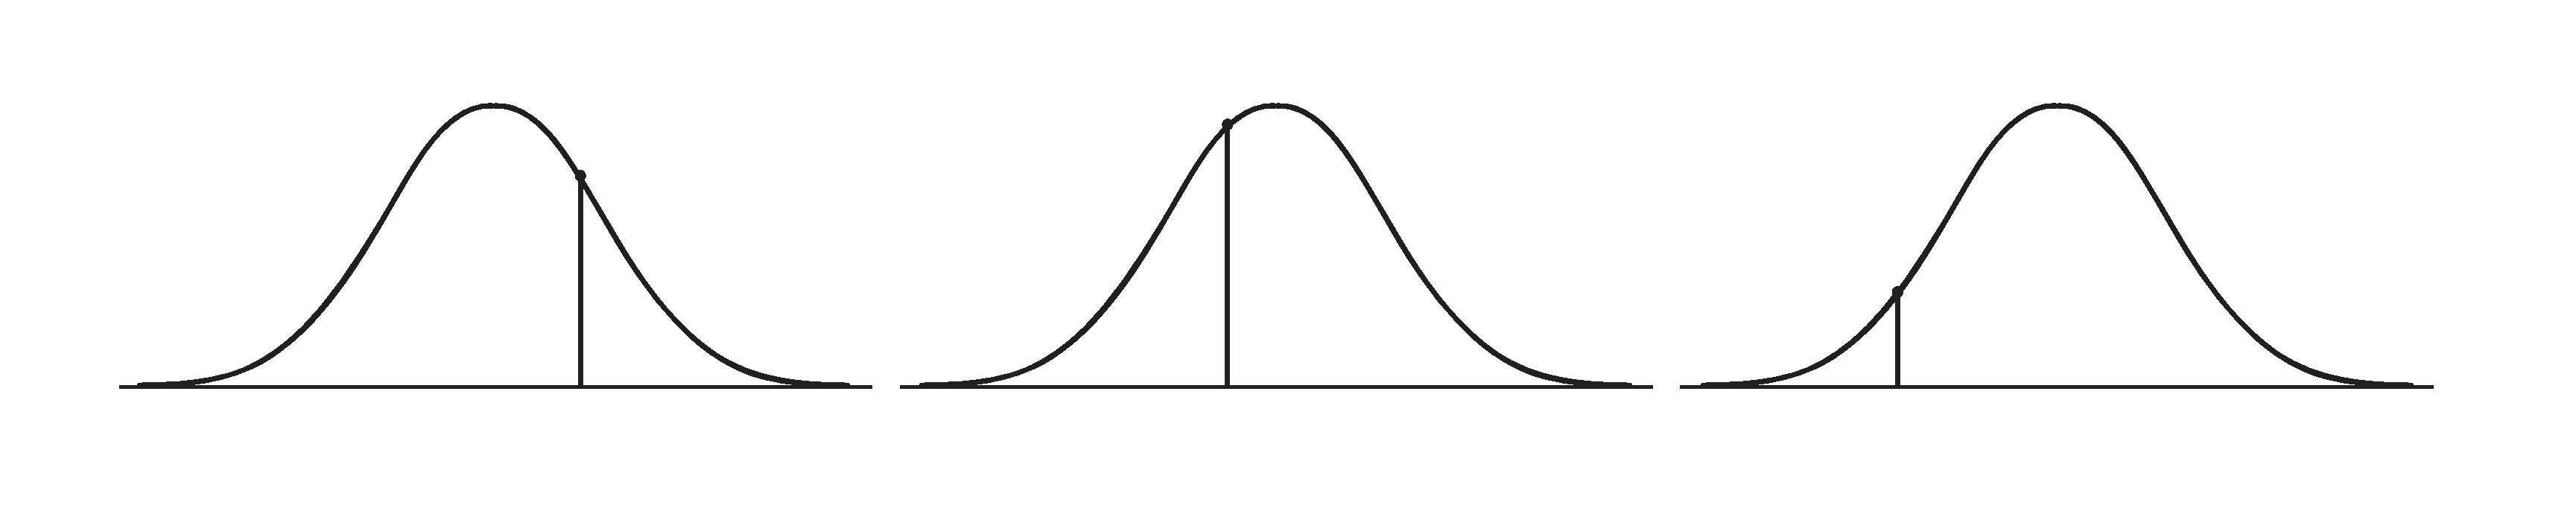
\includegraphics[width=1\textwidth]{diags/fig-hattn-random}
\caption{Selection of three different random samples from a PDF.}
\label{fig:hattn-randomsamp}
\end{figure}
Random sampling from a PDF is illustrated in
\fref{fig:hattn-randomsamp}. It is important to note the following
about random selection:
\begin{enumerate}
\item Two sites that are close to one another may give
dramatically different estimates of ground motion for the same
event. Earthquake hazard and risk values that are computed using
random sampling exhibit a low level of spatial correlation. \item
The number $n_{rand}$ can theoretically take on any value between
$\pm \infty$. Therefore it is possible that estimates of $S_a$ using
\eref{attn:attn-var} can be unrealistically large. \cite{dr_Dhu02b}
overcame this problem by re-scaling the excessively large $S_a$ to
some acceptable level. The re-scaling was performed by the function
\typefunc{pga}{\_cut}{off} which computes a re-scaling parameter
$R_{scale}$ as follows
\begin{equation}
R_{scale} =
\frac{\textrm{\typepar{pga}{\_cut}{off}}}{log(A_{S_a}(0,r_m,R))}.
\end{equation}
The re-scaling parameter is then applied to the entire $S_a$ as
follows
\begin{equation}
log(A_{S_a,new}(T_o,r_m,R)) = R_{scale} \times
log(A_{S_a,old}(T_o,r_m,R)).
\end{equation}
\item There is no effort to account for the likelihood (or
probability) of selecting a particular $n_{rand}$ i.e. a particular
value of the $S_a$ is not weighted against its likelihood. It can be
argued that if enough earthquakes are simulated a range of different
$n_{rand}$ will be taken (high and low) and the overall hazard
and/or risk values will converge to the true ones.
\end{enumerate}


\subsubsection{Spawning\index{response spectral acceleration}
} \label{attn:uncert-pdfchoice}


An alternative technique for incorporating variability relies on
sampling the PDF of the $S_a$. This technique is used by Aon Re
(Mendez, \textit{pers. comm.}, 2003) and is often referred to as
spawning. An integral component of sampling the PDF is the spawning
of events with the event catalogue (see \sref{source:spawning}).
Essentially the approach involves taking a user defined number of
copies of each event. Every event copy is then available for
calculation of hazard (or risk) using a different sample from the
attenuation model PDF.
\begin{enumerate}
\item Firstly the user must define a lower magnitude bound
$m_{bnd}$, a number of samples $n_{smples}$ and a PDF range
$n_\sigma$ (see \sref{source:spawning} for a complete definition).
Recall that \typefunc{fuse}{\_4}{hzd} redefines the event activity
$r_\nu$ using a weight $w_e$, derived by truncating and
re-normalising a standard normal distribution to $\pm n_\sigma$.
\item The $S_a$ is computed as follows
\begin{equation}
\label{attn:uncertainty-pdfsample}
\begin{array}{ll}
log(A_{S_a,i}(T_o,r_m,R)) = \mu_{log(S_a)} - \epsilon_i
\sigma_{log(S_a)}\ & \textrm{for $i=1 \ldots
n_{smples}$} \\
\end{array}
\end{equation}
where
\begin{equation}
\label{attn:uncertainty-def-epsilon}
\begin{array}{ll}
\epsilon_i = -n_\sigma + \frac{\Delta}{2} + (i-1)\Delta &
\textrm{for $i=1 \ldots n_{smples}$} \\
\end{array}
\end{equation}
and
\begin{equation}
\Delta = \frac{2n_\sigma}{n_{smples}}.
\end{equation}
Note that
\ereftwo{attn:uncertainty-pdfsample}{attn:uncertainty-def-epsilon}
ensure that the $S_a$ associated with each of the event copies are
evenly spread across the domain of the attenuation PDF
(\fref{fig:hattn-spawnsamp}). Recall from \sref{source:spawning}
that the event activities $r_\nu$ giving rise to each of the $S_a$
described in \eref{attn:uncertainty-pdfsample} are modified by
\typefunc{fuse}{\_4}{hzd} as follows:
\begin{equation}
r_{\nu,i} = r_{\nu,original} \times w_{e,i}
\end{equation}
\end{enumerate}

For example, assume that there is an event with $r_\nu=0.05$ that
gives rise to \mbox{$\mu_{log(S_a)}=[0.3g, 0.5g, 0.2g]$} at the
periods \mbox{$T_o = [0s,0.3s,1s]$} respectively. Also assume that
the estimates of $\mu_{log(S_a)}$ have the following standard
deviations \mbox{$\sigma_{log(S_a)}=\sigma_a = [0.03,0.04,0.01]$}.
Defining $m_{bnd}=0$, $n_{smples}=5$ and $n_\sigma=2.5$ gives
\begin{equation}
\Delta = \frac{2 \times 2.5}{5} = 1,
\end{equation}

and

\begin{center} $ \begin{array}{ccccc}
i & w_{e,i} & \epsilon_i & r_\nu & log(A_{S_a,i}) \\
\hline
1 & 0.0545 & -2 & 0.0027 & [0.24g, 0.42g, 0.18g] \\
2 & 0.2442 & -1 & 0.0122 & [0.27g, 0.46g, 0.19g] \\
3 & 0.4026 & 0  & 0.0201 & [0.30g, 0.50g, 0.20g] \\
4 & 0.2442 & 1  & 0.0122 & [0.33g, 0.54g, 0.21g] \\
5 & 0.0545 & 2  & 0.0027 & [0.36g, 0.58g, 0.22g] \\
\hline
\end{array}$
\end{center}

\begin{figure}
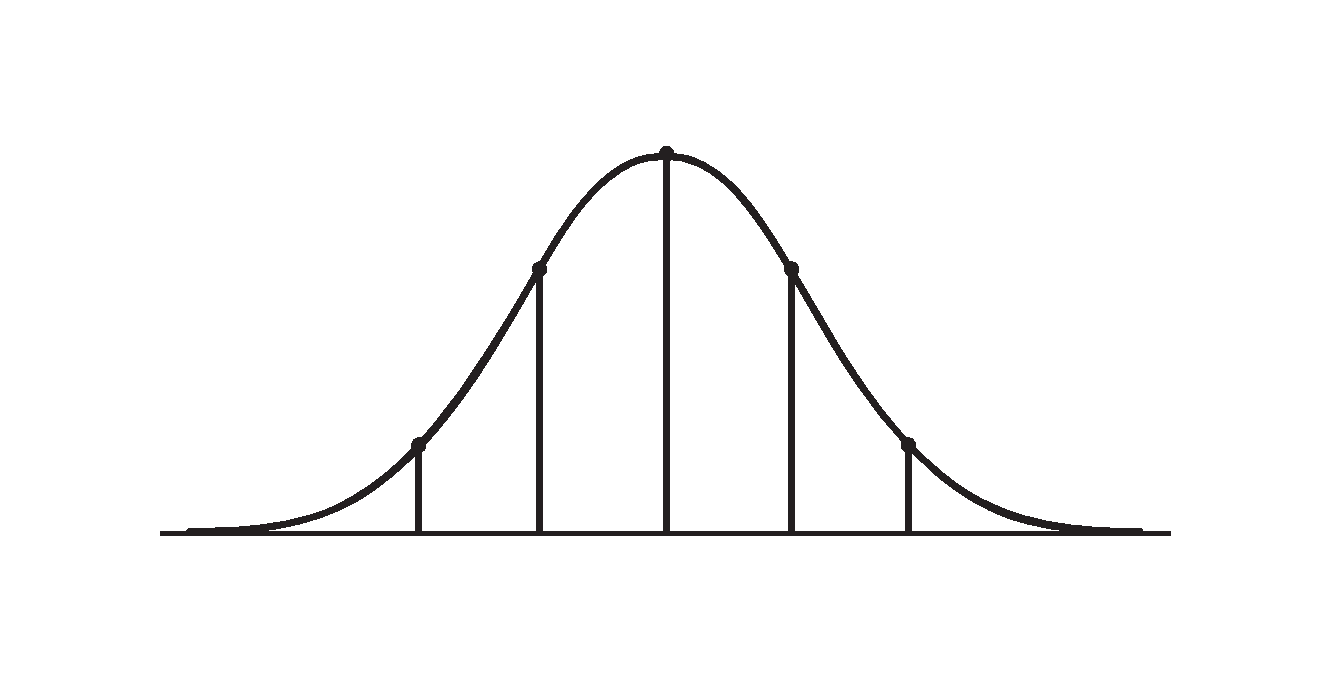
\includegraphics[width=1\textwidth]{diags/fig-hattn-spawning}
\caption{Samples drawn from a PDF using the sampling by spawning
technique with $n_{smples}=5$ and $n_\sigma=2.5$. The width between
the vertical bars is $\Delta$. Note that there is one sample for
each of the five (spawned) copies of the original event.}
\label{fig:hattn-spawnsamp}
\end{figure}

It is important to note the following about spawning:
\begin{enumerate}
\item Sub-sampling the PDF provides a smoother (and repeatable)
estimate of the $S_a$ than random selection
(\sref{attn:uncert-randomchoice}). This equates to a high level of
spatial correlation. \item The range of possible $S_a$ values is
bounded by the $n_\sigma$. \item Estimates of all $S_a$ are weighted
against an event activity $r_\nu$ that accounts for the likelihood
of a particular attenuation being observed. \item The nature of
spawning means that the synthetic event catalogue is copied a number
of times and hence requires more computation time and memory.
\end{enumerate}

\sref{source:spawning} stated that event spawning is conducted when
\typepar{src}{\_eps}{\_switch} is 1 or $2$. When
\typepar{src}{\_eps}{\_switch}$=2$ the spawned values are treated
separately throughout the hazard or risk assessment. When
\typepar{src}{\_eps}{\_switch}$=1$ however, the spawned values are
aggregated again before the hazard or risk assessment is made. This
idea is illustrated in \fref{fig:attn-treecollapse}.

\begin{figure}
 \setlength{\unitlength}{1mm}
(a)  % This is the hazard tree for multi attenuation with collapse

\hspace{4em} \begin{centering}
\begin{picture}(70,30)
% middle branch
\put(0,12){$E_{ij}$} \put(7,13){\vector(1,0){15}}
\put(24,12){$Sa_{ij}^{(2)}$} \put(33,13){\vector(1,0){15}}
\put(50,12){$\widetilde{Sa_{ij}^{(2)}}$} \put(12,14){$w_2$}
% upper branch
\put(7,14){\vector(3,2){15}} \put(24,23){$Sa_{ij}^{(1)}$}
\put(33,24){\vector(1,0){15}}
\put(50,23){$\widetilde{Sa_{ij}^{(1)}}$}
\put(11,20){\rotatebox{30}{$w_1$}}
% lower branch
\put(7,12){\vector(3,-2){15}} \put(24,0){$Sa_{ij}^{(3)}$}
\put(33,1){\vector(1,0){15}} \put(50,0){$\widetilde{Sa_{ij}^{(3)}}$}
\put(11,5){\rotatebox{-30}{$w_3$}}
% concatenation at end
\put(61,5){\scalebox{1.2}[6.5]{\}}} \put(65,12){$ {\displaystyle
\widetilde{Sa_{ij}} = \sum_{k=1}^{3}w_k\widetilde{Sa_k} } $}
\end{picture}
\end{centering}

\vspace{0.8em}
(b) % This is the hazard tree for multi attenuation with NO collapse

\hspace{4em} \begin{centering}
\begin{picture}(70,30)
% middle branch
\put(0,12){$E_{ij}$} \put(7,13){\vector(1,0){15}}
\put(24,12){$Sa_{ij}^{(2)}$} \put(33,13){\vector(1,0){15}}
\put(50,12){$\widetilde{Sa_{ij}^{(2)}}$} \put(12,14){$w_2$}
% upper branch
\put(7,14){\vector(3,2){15}} \put(24,23){$Sa_{ij}^{(1)}$}
\put(33,24){\vector(1,0){15}}
\put(50,23){$\widetilde{Sa_{ij}^{(1)}}$}
\put(11,20){\rotatebox{30}{$w_1$}}
% lower branch
\put(7,12){\vector(3,-2){15}} \put(24,0){$Sa_{ij}^{(3)}$}
\put(33,1){\vector(1,0){15}} \put(50,0){$\widetilde{Sa_{ij}^{(3)}}$}
\put(11,5){\rotatebox{-30}{$w_3$}}
\end{picture}
\end{centering}

\vspace{0.8em}
(c) % This is the risk tree for multi attenuation with collapse

\hspace{4em} \begin{centering}
\begin{picture}(70,30)
% middle branch
\put(0,12){$E_{ij}$} \put(7,13){\vector(1,0){15}}
\put(24,12){$Sa_{ij}^{(2)}$} \put(33,13){\vector(1,0){15}}
\put(50,12){$\widetilde{Sa_{ij}^{(2)}}$} \put(12,14){$w_2$}
\put(60,13){\vector(1,0){15}} \put(77,12){$L_{ij}^{(2)}$}
% upper branch
\put(7,14){\vector(3,2){15}} \put(24,23){$Sa_{ij}^{(1)}$}
\put(33,24){\vector(1,0){15}}
\put(50,23){$\widetilde{Sa_{ij}^{(1)}}$}
\put(11,20){\rotatebox{30}{$w_1$}} \put(60,24){\vector(1,0){15}}
\put(77,23){$L_{ij}^{(1)}$}
% lower branch
\put(7,12){\vector(3,-2){15}} \put(24,0){$Sa_{ij}^{(3)}$}
\put(33,1){\vector(1,0){15}} \put(50,0){$\widetilde{Sa_{ij}^{(3)}}$}
\put(11,5){\rotatebox{-30}{$w_3$}} \put(60,1){\vector(1,0){15}}
\put(77,0){$L_{ij}^{(3)}$}
% concatenation at end
\put(86,5){\scalebox{1.2}[6.5]{\}}} \put(90,12){$ {\displaystyle
 L_{ij} = \sum_{k=1}^{3}w_kL_k } $}
\end{picture}
\end{centering}

\vspace{0.8em}
(d)  % This is the risk tree for multi attenuation with NO collapse


\hspace{4em}\begin{picture}(70,30)
\begin{centering}
% middle branch
\put(0,12){$E_{ij}$} \put(7,13){\vector(1,0){15}}
\put(24,12){$Sa_{ij}^{(2)}$} \put(33,13){\vector(1,0){15}}
\put(50,12){$\widetilde{Sa_{ij}^{(2)}}$} \put(12,14){$w_2$}
\put(60,13){\vector(1,0){15}} \put(77,12){$L_{ij}^{(2)}$}
% upper branch
\put(7,14){\vector(3,2){15}} \put(24,23){$Sa_{ij}^{(1)}$}
\put(33,24){\vector(1,0){15}}
\put(50,23){$\widetilde{Sa_{ij}^{(1)}}$}
\put(11,20){\rotatebox{30}{$w_1$}} \put(60,24){\vector(1,0){15}}
\put(77,23){$L_{ij}^{(1)}$}
% lower branch
\put(7,12){\vector(3,-2){15}} \put(24,0){$Sa_{ij}^{(3)}$}
\put(33,1){\vector(1,0){15}} \put(50,0){$\widetilde{Sa_{ij}^{(3)}}$}
\put(11,5){\rotatebox{-30}{$w_3$}} \put(60,1){\vector(1,0){15}}
\put(77,0){$L_{ij}^{(3)}$}
\end{centering}
\end{picture}


\caption{The application of spawning to a single synthetic
earthquake $E_{ij}$;(a) the collapse of spawned samples for hazard
(\typeparcaption{src}{\_eps}{\_switch}$=1$); (b) hazard spawning
without collapse (\typeparcaption{src}{\_eps}{\_switch}$=2$); (c)
the collapse of spawned samples for risk
(\typeparcaption{src}{\_eps}{\_switch}$=1$); and (d) risk spawning
without collapse (\typeparcaption{src}{\_eps}{\_switch}$=2$). The
illustrated procedure is repeated for $N_s$ events in the event
catalogue and the techniques of \cref{ch:risk} used to assess the
hazard or risk.} \label{fig:attn-treecollapse}
\end{figure}

\subsection{Incorporating
epistemic uncertainty} \label{sec:attn-multi-attnmodels}

The use of attenuation models in the EQRM is controlled by the
\typeself{set}{da}{ta} parameter \typepar{atten}{uation}{\_flag}.
Recall from \sref{sec:application-setdata} that
\typepar{atten}{uation}{\_flag} is a two row matrix with one column
for each attenuation model to be used. The format of
\typepar{atten}{uation}{\_flag} is
\begin{center}
\begin{math}
%\label{fig:attn-sa-matrix}
 \left[ \begin{array}{ccccc}
P_1 & P_2 &  \hdots & P_n \\
w_{a,1} & w_{a,2} &  \hdots & w_{a,n} \\
\end{array} \right],
\end{math}
\end{center}
where the integers $\{P_i\}_{i=1}^n$ are pointers to the attenuation
model (see \tref{tab:attn-flags}) and the real numbers
$\{w_{a,i}\}_{i=1}^n$ are weights for the respective attenuation
models. Note that the weights $w_i$ must either be all positive or
all negative and
\begin{equation}
\left|\sum_{i=1}^{n}w_{a,i}\right| = 1.
\end{equation}
\begin{table}
\caption{Pointers to attenuation models for use in the first row of
\typeparcaption{atten}{uation}{\_flag}.} \vspace{0.8em}
\label{tab:attn-flags}
\begin{center}
\begin{tabular}{|c|c|c|}
\hline \textbf{Motion} & \textbf{pointer} & \textbf{model} \\
\hline
 & 0 & \cite{dr_Gaull90a} PGA with $S_a$ extension\\
 & 1 & \cite{dr_Toro97a} \\
$S_a$ & 2 & \cite{dr_Atkinson97a} \\
 & 3 & \cite{dr_Sadigh97a} \\
 & 4 & \cite{dr_Somerville01a} \\
\hline
 $\Imm$ & 100 & \cite{dr_Gaull90a} \\
\hline
\end{tabular}
\end{center}
\end{table}

\begin{table}
\caption{Attenuation region (\typeparcaption{attn}{\_reg}{ion})
options for each of the attenuation models.} \vspace{0.8em}
\label{tab:attn-regions}
\begin{center}
\begin{tabular}{|c|c|l|}
\hline \textbf{attenuation} & \textbf{attenuation} & \textbf{\texttt{attn\_region}} \\
\textbf{pointer} & \textbf{model} & \textbf{} \\
\hline
0   &  & 1 $\Rightarrow$ Western Australia  \\
or & \cite{dr_Gaull90a} & 2 $\Rightarrow$ Northeastern Australia\\
100 & & 3 $\Rightarrow$ Indonesia\\
 & & 4 $\Rightarrow$ Southeastern Australia\\
\hline
1 & \cite{dr_Toro97a} & 1 $\Rightarrow$ Mid-Continent $M_o$ \\
\hline
2 & \cite{dr_Atkinson97a} & 1 $\Rightarrow$ No published options \\
\hline
3 & \cite{dr_Sadigh97a} & 1 $\Rightarrow$ No published options \\
\hline
 &  & 1 $\Rightarrow$ Nonrift - Horizontal\\
4 & \cite{dr_Somerville01a} & 2 $\Rightarrow$ Rift -- Horizontal\\
 & & 3 $\Rightarrow$ Nonrift -- Vertical\\
 & & 4 $\Rightarrow$ Rift --Vertical\\
\hline
\end{tabular}
\end{center}
\end{table}

The mechanism for using more than one attenuation model is similar
to the mechanism used for spawning (see
\sref{attn:uncert-pdfchoice}). That is, the event catalogue is
copied $n$ times (once for each attenuation model) and the
appropriate attenuation model applied to its respective copy. The
values of ground motion (loss for risk) can then be treated
independently for the hazard/risk calculation (if
$\sum_{i=1}^{n}w_{a,i} = -1$) or aggregated before the hazard/risk
assessment is undertaken (if $\sum_{i=1}^{n}w_{a,i} = 1$). This
notion of logic tree collapse is described by
\fref{fig:attn-treecollapse}.

\clearpage
\newpage
\section{Key functions, flags and parameters}

\begin{tabular}{llp{0.55\textwidth}}
\hline
\textbf{Name} & \textbf{Type} & \textbf{Description} \\
\hline
\keyrowsep \typefunc{do}{\_ana}{lysis} & Function & The main driving function for modelling earthquake hazard or risk. \\
\keyrowsep \typefunc{do}{\_all}{dist} & Function & Computes the Joyner-Boore and Rupture Distance from a site to every event. \\
\keyrowsep \typefunc{prep}{\_at}{tn} & Function & Prepares the attenuation coefficients by interpolating them to periods of interest $T_o$. \\
\keyrowsep \typefunc{m}{w2}{ml} & Function & Converts moment magnitude $r_m$ to local magnitude $r_{m_l}$. \\
\keyrowsep \typefunc{do}{\_atten}{uation} & Function & Controls the selection of attenuation models for evaluation and assembles outputs. \\
\keyrowsep \splitrowfunc{attn\_prepcoeff}{\_toro} & Function & Preparation of attenuation coefficients for \cite{dr_Toro97a}. \\
\keyrowsep \splitrowfunc{attn\_allpervec}{\_toro} & Function & Computes \cite{dr_Toro97a} attenuation. \\
\keyrowsep \splitrowfunc{attn\_preptoro}{\_aleatory1} & Function & Computes $\sigma_{a,r_m}$ for use with \cite{dr_Toro97a} attenuation. \\
\keyrowsep \splitrowfunc{attn\_preptoro}{\_aleatory2} & Function & Computes $\sigma_{a,\Rjb}$ for use with \cite{dr_Toro97a} attenuation. \\
\keyrowsep \splitrowfunc{attn\_preptoro}{\_epistemic} & Function & Computes $\sigma_{e,r_m}$ for use with \cite{dr_Toro97a} attenuation. \\
\keyrowsep \splitrowfunc{attn\_allpervec}{\_gaull} & Function & Computes \cite{dr_Gaull90a} attenuation. \\
\keyrowsep \typefunc{aus}{\_pesh}{new} & Function & Extends $PGA$ to standard $\mu_{log(S_a)}$. \\
\keyrowsep \splitrowfunc{attn\_prepcoeff}{\_atkboore} & Function & Preparation of attenuation coefficients for \cite{dr_Atkinson97a}.\\
\keyrowsep \splitrowfunc{attn\_allpervec}{\_atkboore} & Function & Computes \cite{dr_Atkinson97a} attenuation. \\
\keyrowsep \splitrowfunc{attn\_prep\_atkboore}{\_aleatory} & Function & Computes $\sigma_a$ for use with \cite{dr_Atkinson97a} attenuation. \\
\keyrowsep \splitrowfunc{attn\_prepcoeff}{\_sadigh} & Function & Preparation of attenuation coefficients for \cite{dr_Sadigh97a}. \\
\keyrowsep \splitrowfunc{attn\_allpervec}{\_sadigh} & Function & Computes \cite{dr_Sadigh97a} attenuation. \\
\end{tabular}

\begin{tabular}{llp{0.55\textwidth}}
\keyrowsep \splitrowfunc{attn\_prep\_sadigh}{\_uncertainty} & Function & Prepares uncertainty coefficients for \cite{dr_Sadigh97a} attenuation. \\
\keyrowsep \typefunc{pga}{\_cut}{off} & Function & Re-scales the $S_a$ such that PGA $\leq$ \typepar{pga}{cut}{off}. \\
\keyrowsep \splitrowfunc{attn\_toro\_mid}{continent\_momag} & Par File & Stores attenuation coefficients for \cite{dr_Toro97a} attenuation. \\
\keyrowsep \splitrowfunc{attn\_atkboore}{\_momag} & Par File & Stores attenuation coefficients for \cite{dr_Atkinson97a} attenuation. \\
\keyrowsep \splitrowfunc{attn\_sadigh\_coeff}{\_momag\_less65} & Par File & Stores attenuation coefficients for \cite{dr_Sadigh97a} attenuation. \\
\keyrowsep \splitrowfunc{attn\_sadigh\_coeff}{\_momag\_great65} & Par File & Stores attenuation coefficients for \cite{dr_Sadigh97a} attenuation. \\
\keyrowsep \typepar{per}{io}{ds} & Par & Periods at which to compute $S_a$. \\
\keyrowsep \typepar{atten}{uation}{\_flag} & Par & Defines the attenuation models to be used as well as their respective weights. \\
\keyrowsep \typepar{attn}{\_reg}{ion} & Par & Flag to assign different attenuation regions for \cite{dr_Gaull90a} attenuation.\\
\keyrowsep \typepar{var}{\_attn}{\_flag} & Par & Variability in evaluation of the attenuation model. \\
\keyrowsep \typepar{var}{\_attn}{\_method} & Par & Selects the technique for incorporating variability. \\
  \hline
\end{tabular}







%%% Local Variables:
%%% mode: latex
%%% TeX-master: "eqrmtech"
%%% End:

%\chapter{Regolith amplification}
\label{ch:reg}


\section{Overview}

Regolith is defined as the soil, geological sediments and
weathered rock that overly the un-weathered bedrock. It is well
documented that the presence of regolith can increase the level of
ground shaking experienced during an earthquake
(\citealt{dr_Borcherdt76a}; \citealt{dr_Murphy71a}).  For example,
studies in the San Fernando Valley and Los Angeles Basin, U.S.A.,
have demonstrated that the damage patterns observed during the
1994 Northridge, California earthquake can be strongly correlated
to site-response of local regolith \citep{dr_Meremonte96a}.
Consequently, including the effect of regolith on earthquake
ground shaking is an important component of any seismic hazard or
risk analysis.

\subsection{Background theory}

An amplification factor can be used to transfer the earthquake
motion from the bedrock to the regolith surface. Amplification
factors are influenced by the regolith at the site of interest,
the magnitude $r_m$ of the event and the PGA for the event-site
combination. For simplicity, the geographical region of interest
is usually separated into five or six site-classes inside which
the regolith is assumed to be the same. The EQRM application does
not compute the amplification factors (or level of amplification).
Such calculations must be conducted off-line and the results (or
amplification factors) made available to the EQRM application. The
interested reader is referred to \citet{dr_Robinson06a} for a
detailed description of the equivalent linear technique for
computing amplification factors. \citet{dr_Dhu02b} discuss the
classification of site classes and the application of
amplification factors to a probabilistic seismic hazard analysis.
\fref{fig:regolith-newcexample-crosssection} illustrates the
geotechnical cross section for all of the site classes in the
Newcastle and Lake Macquarie region, and
\fref{fig:regolith-newcexample-ampfactors} shows an example of the
amplification factors use in the same study.


\begin{figure}
\begin{center}
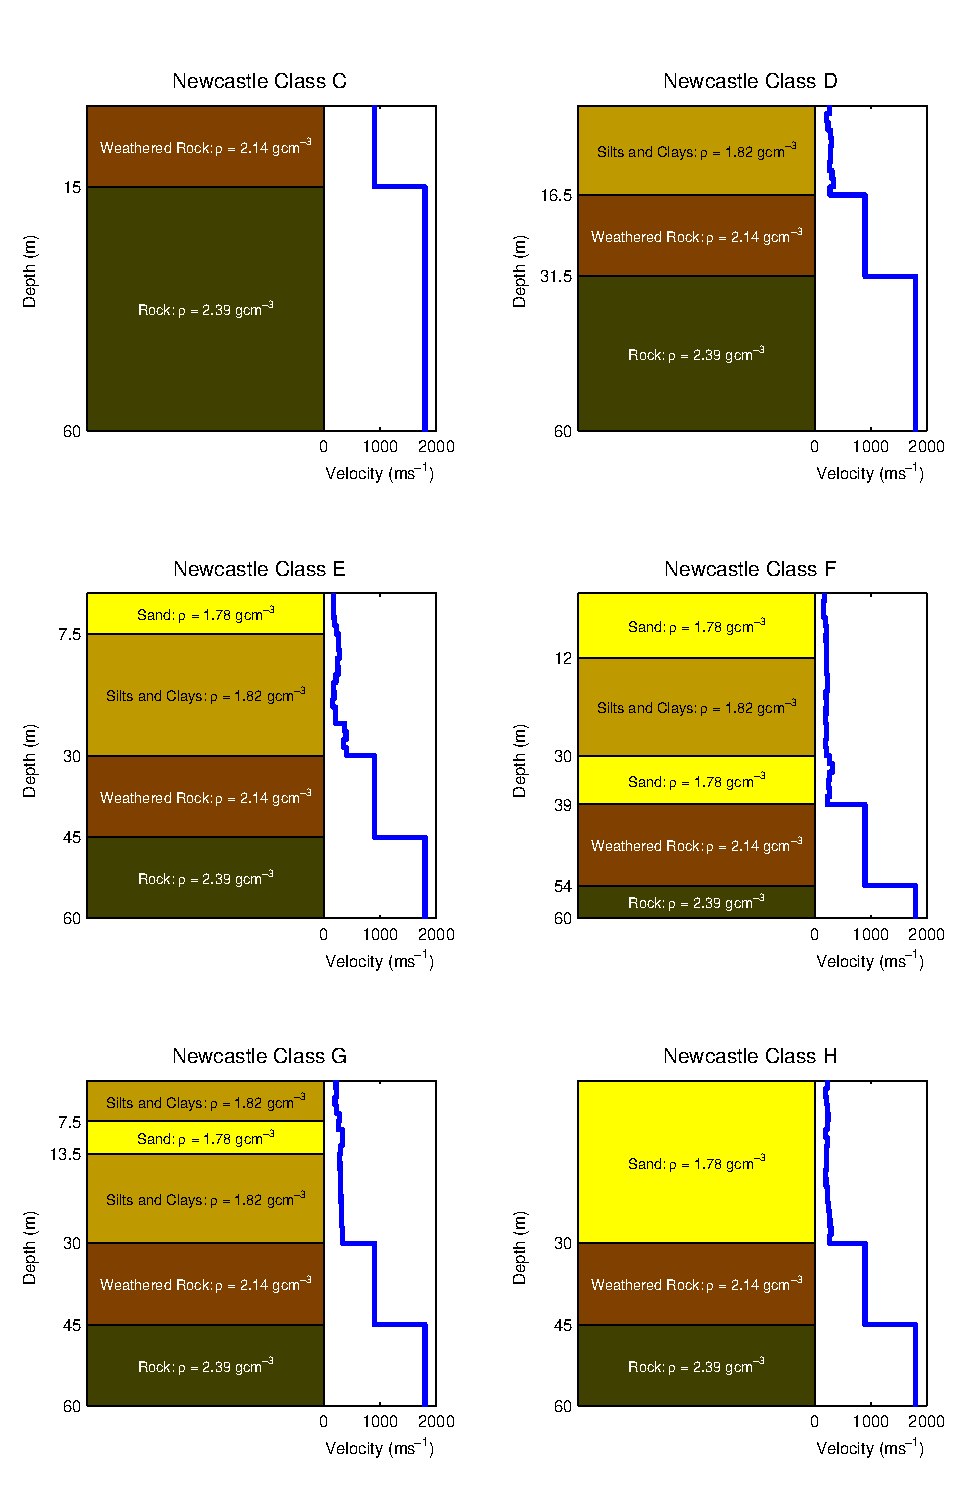
\includegraphics[width=0.6\textheight]{fig-hregolith-crosssections}
\end{center}
\caption{Cross sections of the 6 site classes used in the
Newcastle and Lake Macquarie study \citep{dr_Dhu02b}. }
\label{fig:regolith-newcexample-crosssection}
\end{figure}

\begin{figure}
\begin{center}
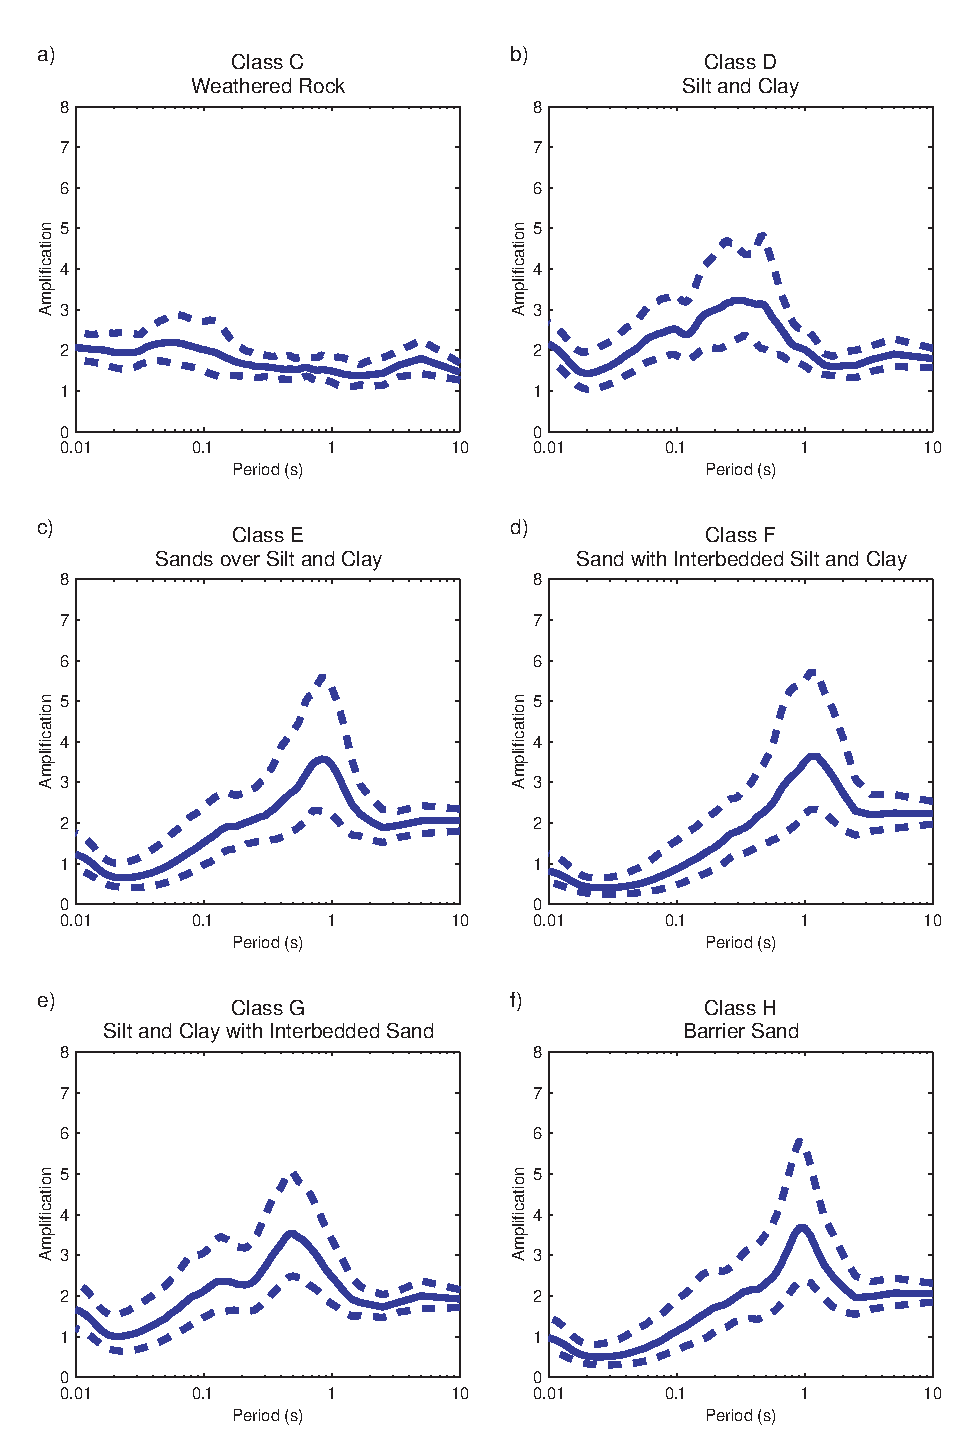
\includegraphics[width=0.6\textheight]{fig-hregolith-ampfactors}
\end{center}
\caption{Example amplification factors for the site classes shown
in \fref{fig:regolith-newcexample-crosssection}. Note that the
amplification factors are for moment magnitude 5.5 and PGA
$0.25g$. } \label{fig:regolith-newcexample-ampfactors}
\end{figure}


\section{Implementation}

As with the attenuation, the implementation of the amplification
factors (for both hazard and risk assessments) has been done in a
two step process as follows:
\begin{enumerate}
\item The preparation of the amplification factors
conducted before entering a loop over sites. \item Application of
the amplification factors to compute $A_{S_a,soil}(T_o,r_m,R)$ at
each site conducted within a loop over sites.
\end{enumerate}

The preparation of amplification factors involves interpolating each
to the periods defined in the the EQRM control file parameter:
\typeself{atten-periods} (see ~\sref{sec:application-EQRMcf}). The
application of the amplification factors is carried out immediately
after the evaluation of the attenuation model. The process is
described for a specific site located within a known Site Class:
\begin{enumerate}
\item Bin all of the events in the event catalogue into the
bedrock PGA and moment magnitude bins defined by the bin centroids
in \typevar{}{}{pga\_bins} and \typevar{}{}{moment\_magnitude\_bins}
respectively (see ~\sref{sec:-appl-amplification}). Note that the
end points of the 'central' bins are assumed to be half way between
the bin centroids. The first and last bins extend to negative and
positive infinity respectively.
\item Use a nested loop over all PGA bins (upper loop) and moment
magnitude bins (lower loop) and apply the amplification factor as
follows:
\begin{equation}
S_{a,soil}(T_o,r_m,R)= F_{amp}(T_o,r_m^*,PGA^*) \times
S_{a,bedrock}(T_o,r_m,R),
\end{equation}
where $r_m^*$ and $PGA^*$ are the centroids of the bins containing
$r_m$ and \newline $S_{a,bedrock}(0,r_m,R)$ respectively. The
$F_{amp}$ represents the exponential of `some selection' of
amplification factor from the distribution \newline \mbox{$N \sim
(\mu_{log(F)}(T_o,r_m^*,PGA^*),\sigma_{log(F)}(T_o,r_m^*,PGA^*))$}.
The actual selection  made will depend on the method used to
incorporate uncertainty (see \sref{sec:regolith-incorp-unc}).
\end{enumerate}
Notice that the use of $N \sim (\mu_{log(F)},\sigma_{log(F)})$
equates to the assumption that the amplification factors are
log-normally distributed.

\section{Incorporating aleatory uncertainty}
\label{sec:regolith-incorp-unc}


In theory, both the random selection and PDF sampling methods
described in \sref{attn:uncertainty} could be used to incorporate
aleatory uncertainty in amplification factors. Some care will need
to be taken if the PDF sampling technique is to be used for
incorporating uncertainty at several levels  of computation (e.g.
for attenuation and amplification) due to the need to spawn the
event catalogue (see \sref{source:spawning}) at every level. Such
iterative spawning may lead to a `blow-out' in the size of the event
catalogue and hence the computation time. Currently only the random
selection technique is available for use with the amplification
factors in the EQRM application.

As with the application of an attenuation model, the EQRM applies
$PGA_{cut}$ to $S_{a,soil}(T_o,r_m,R)$ after applying the
amplification factor. This accounts for any unrealistically high
selection of amplification factor. A secondary upper cut-off
facility exists and involves the use of the
\typepar{amp}{\_max}{\_factor}(see \sref{sec:application-EQRMcf}).
The \typepar{amp}{\_max}{\_factor} parameter is applied directly to
the amplification factor as follows:
\begin{equation}
\label{eq:regolith-maxampfactor}
F_{new}(T_o,r_m^*,PGA^*) = \left \{ \begin{array}{ll} F_{old} & \textrm{$\forall$ \hspace{0.2em} $T_o$ s.t. $F_{amp,old}<$\typepar{amp}{\_max}{\_factor}} \\
\textrm{\typepar{amp}{\_max}{\_factor}} & \textrm{$\forall$ \hspace{0.2em} $T_o$ s.t. $F_{amp,old} \geq $ \typepar{amp}{\_max}{\_factor}} \\
\end{array} \right.
\end{equation}
or brevity the functional reference to $r_m^*$ and $PGA^*$ in
$F_{new}$ and $F_{old}$ in
\ereftwo{eq:regolith-maxampfactor}{eq:regolith-minampfactor} refers
to the fact that these values represent the bin centroids of
\typevar{}{}{moment\_magnitude\_bins} and \typevar{p}{ga}{\_bins}
respectively. In most simulations the secondary cutoff is not used
since $PGA_{cut}$ handles scaling for an upper bound. Ignoring
\typepar{amp}{\_max}{\_factor} is achieved by setting it to to a
very high number (e.g. \typepar{amp}{\_max}{\_factor}=10000). In
contrast, there is another parameter in the EQRM control file known
as \typepar{amp}{\_min}{\_factor} which is commonly utilised within
the EQRM application. This parameter stops the selection of any
unrealistically low selections of the amplification factor. The
\typepar{amp}{\_min}{\_factor} is commonly set to around 0.6. It is
applied as follows:
\begin{equation}
\label{eq:regolith-minampfactor}
F_{new}(T_o,r_m^*,PGA^*) = \left \{ \begin{array}{ll} F_{old} & \textrm{$\forall$ \hspace{0.2em} $T_o$ s.t. $F_{amp,old} >$\typepar{amp}{\_min}{\_factor}} \\
\textrm{\typepar{amp}{\_min}{\_factor}} & \textrm{$\forall$ \hspace{0.2em} $T_o$ s.t. $F_{amp,old} \leq $ \typepar{amp}{\_min}{\_factor}} \\
\end{array} \right.
\end{equation}
Note that a value of \mbox{$F<1$} leads to a de-amplification of
the bedrock motion.

\chapter{Building damage}
\label{ch:damage}

\section{Introduction}
\label{sec:v-dam-intro}

This chapter describes the modelling of building damage. The
method is based on the HAZUS methodology \citep{dr_FEMA99b} with a
few modifications to suit the Monte-Carlo approach used in the
EQRM. The modifications are discussed at the end of this chapter.

The Capacity Spectrum Method\index{capacity spectrum method}
(\citealp{dr_FEMA99b}; \citealp{dr_Kircher97a}) is used to obtain
the peak building displacement and acceleration corresponding to
each earthquake. The peak displacement\index{peak displacement}
and acceleration are the dependent variables for fragility
curve\index{fragility curves}s \citep{dr_Kircher97a} which give
probabilities of being in certain damage states, for different
types of damage, structural (damage to main structure) and
drift-sensitive and acceleration-sensitive non-structural damage
(e.g. damage to non-structural internal walls).


%%%%%%%%%%%%%%%%%%%%%%%%%%%%%%%%%%%%%%%%%%%%%%%%%%%5
\section{The capacity spectrum method}
\label{sec:v-dam-capspect}

The capacity spectrum method\index{capacity spectrum method} is
used to find the peak displacement\index{peak displacement} and
peak acceleration\index{peak acceleration} for each
earthquake-building pair. To use this technique each building is
approximated by a single degree of freedom oscillator (SDOF)
\citep{dr_Chopra01c}.

A building's capacity (or response) to an incoming seismic wave,
is defined by the capacity curve\index{capacity curve}, a
monotonic increasing curve giving the $S_a$ as a function of the
spectral displacement\index{response spectral displacement} $S_d$.
The response spectral acceleration\index{response spectral
acceleration} ($S_a$) normally plotted against building period is
plotted against spectral displacement\index{response spectral
displacement} $S_d$ to describe the `earthquake motion'. When
plotted this way the $S_a vs S_d$ plot is known as the demand
curve\index{demand curve}. The peak displacement\index{peak
displacement} and acceleration experienced by the building as a
result of the `induced motion' is modelled by the intersection of
the capacity curve\index{capacity curve} with the demand
curve\index{demand curve} (\fref{fig:vdamage-capspect}).

The response spectral acceleration\index{response spectral
acceleration} curve is normally defined by the attenuation model
with $5\%$ damping.  The actual damping generated by a building
differs from $5\%$ and is a function of the building attributes
such as structural type (see \cref{ch:grids}). The capacity
spectrum method\index{capacity spectrum method} allows for this
variation by adjusting the damping (see
\sref{subsec:v-dam-damping}).

\begin{figure}[htp]
\centering \psfrag{point}{$(S_d^*, S_a^*)$}
\psfrag{buildingcap}{capacity curve} \psfrag{response}{demand
curve}
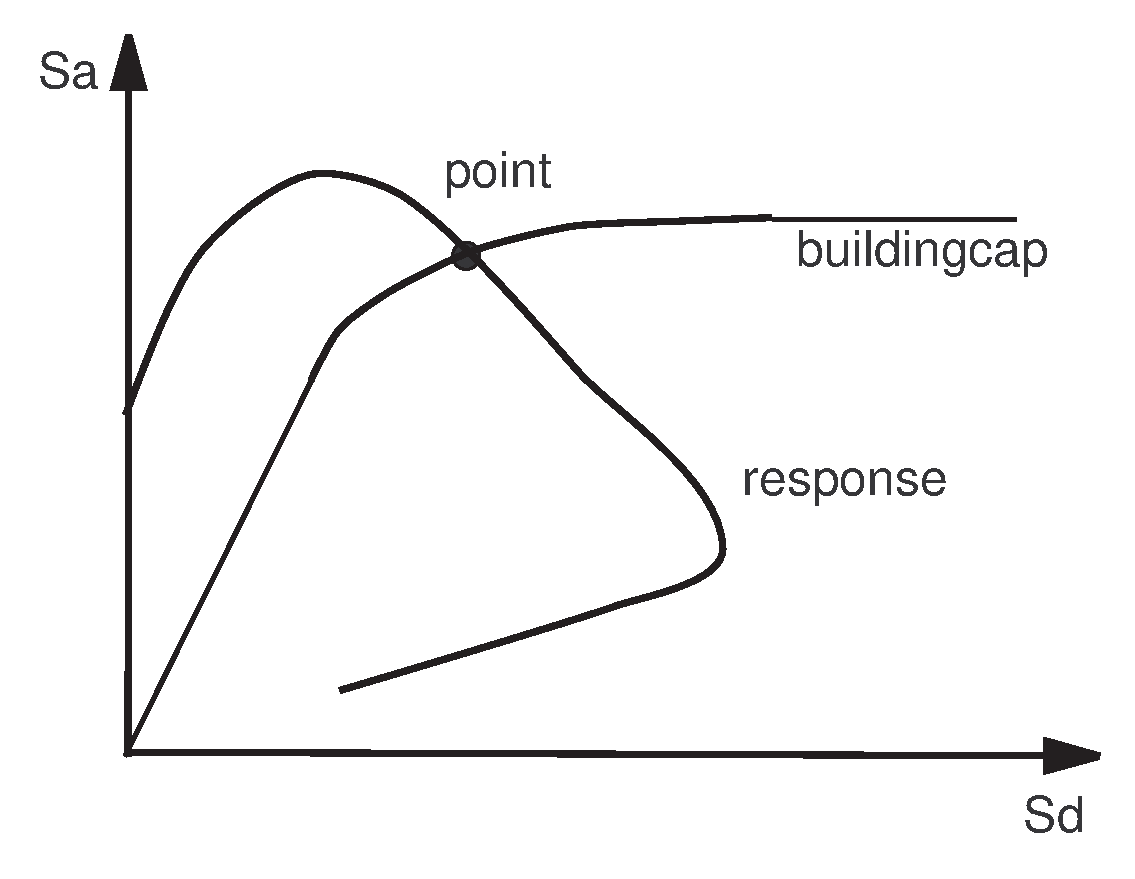
\includegraphics[height=0.3\textheight]{fig-vdamage-capspect}
\caption{The capacity spectrum method\index{capacity spectrum
method}.} \label{fig:vdamage-capspect}
\end{figure}


\fref{fig:vdamage-capspect} illustrates the intersection of the
capacity curve\index{capacity curve} with the demand
curve\index{demand curve}.  In the elastic region (or linear
component) of the capacity curve\index{capacity curve} the
intersection between the capacity curve\index{capacity curve} and
the appropriately damped demand curve\index{demand curve} occurs
at a period corresponding to the natural period of the building.
If the intersection occurs in the nonlinear plastic deformation
region, hysteretic damping results in a larger component of the
earthquakes energy being absorbed through damping in the building.
In an equivalent linear approach, this effectively reduces the
natural period of the building.


\subsection{The building capacity curve\index{capacity curve}}

The building capacity curve\index{capacity curve}\index{building
capacity curve\index{capacity curve}} is defined by two points:
the yield point $(D_y, A_y)$ and the ultimate point $(D_u, A_u)$.
For displacements below the yield point the building response is
elastic and the capacity curve\index{capacity curve} represented
by a straight line. For displacement amplitudes greater than the
yield point nonlinear effects such as plastic deformation cause
the rate of increase to reduce. The curve asymptotes towards the
ultimate point (see \fref{fig:vdamage-cap}).

\begin{figure}[htp]
\centering
\psfrag{yield}{$(D_y, A_y)$}
\psfrag{ult}{$(D_u, A_u)$}
\includegraphics[height=0.3\textheight]{fig-vdamage-cap}
\caption{The graph of a typical building capacity
curve\index{capacity curve}, defined by
  the yield point $(D_y, A_y)$ and the ultimate point $(D_u, A_u)$.
  Note that the straight line between the yield point and the origin
  represents elastic behavior of the building. }
\label{fig:vdamage-cap}
\end{figure}


The yield point and ultimate point are defined in terms of the
building parameters as: $$ \begin{array}{rl}
 A_y = \frac{C_s\gamma}{\alpha_1} & [g],  \vspace{0.5em} \\
 D_y = \frac{1000}{4\pi^2}9.8A_y T_e^2 & [mm],\vspace{0.3em} \\
 A_u = \lambda A_y & [g], \vspace{0.3em} \\
 D_u = \lambda\mu D_y & [mm], \\
 \end{array}
$$
where the building parameters
\begin{align*}
C_s &= \text{design strength coefficient (fraction of the building weight)},\\
T_e &= \text{natural elastic building period (seconds)},\\
\alpha_1 &= \text{fraction of building weight participating in the
  first mode},\\
\alpha_2 &= \text{fraction of the effective building height to
building displacement},\\
\gamma &= \text{over-strength factor---yield to design strength ratio},\\
\lambda &= \text{over-strength factor---ultimate to yield strength ratio},\\
\mu &= \text{ductility factor},
\end{align*}
are given for several classes of building construction types
(\sref{sec:grids-constructionclass}). Note that the parameter
$\alpha_2$ is not used here, rather it is used to define the
appropriate damage ratios (see \eref{eq:damage-dstate}).


\subsubsection{Fitting the building capacity curve\index{capacity curve}}

The capacity curve\index{capacity curve} is composed of three
parts: a straight line to the yield point, a curved part from the
yield point to the ultimate point, and a horizontal line from the
ultimate point.


An exponential function is used to represent the curved part of
the building capacity curve\index{capacity curve}.  When defining
the curved section it is desirable that it has and identical slope
to the elastic part at the yield point and that its slope
approaches zeros at the ultimate point. We cannot satisfy all
these conditions with just three constants, however, we can
satisfy the condition of the curves matching at the ultimate point
approximately.

The form of the exponential curve is
$$
 y = c + a e^{-bx}
$$
where the constants $a$, $b$, and $c$ are given by
\begin{equation}
c = A_u,\quad b = \frac{k}{A_u-A_y}, \quad
a = (A_y-A_u)e^{b D_y}
\end{equation}
where $k = A_y/D_y$.

To obtain this, the following equation follows from the curves
joining at the ultimate points
$$
 c+ae^{-bD_u} = A_u.
$$
If we neglect the $e^{-bD_u}$ term, then $c=A_u$. From the
equation for the yield point we then obtain $A_u-A_y =
-ae^{-bD_y}$. From the equation that the slopes match at the yield
point we obtain $k = -abe^{-bD_y}$, where $k=A_y/D_y$ is the slope
of the elastic linear part of the capacity curve\index{capacity
curve}. Eliminating the exponential term from both these equations
gives the value of $b$, and the expression for $a$ follows. The
condition that the slope is zero at the ultimate point is
consistent with the assumption of neglecting the term $e^{-bD_u}$.
This will be true provided
$$
 \frac{D_u/D_y}{A_u/A_y-1} \gg 1.
$$
which will be generally true when the ultimate point is far from the
yield point.


\subsubsection{Variability of the capacity curve\index{capacity curve}s}
\label{sec:dam-capacity-var}

The uncertainty of the peak response of the building to a given
ground-shaking is incorporated by using a log-normal distribution
of building capacity curve\index{capacity curve}s with a
log-normal standard deviation parameter $\beta=0.3$. This value is
taken from \cite{dr_FEMA99b} for pre-code buildings with a value
of 0.25 recommended for buildings constructed in alignment with
building codes. HAZUS gives no explanation or reference to how
these values were obtained. It was recommended in the Engineers'
workshop, \cite{dr_Stehle01a}, that a value $\beta=0.4$ be used
for Australian buildings, but there was no justification given for
this, so a value of $\beta=0.3$ has been retained.

The variability of the building capacity curve\index{capacity
curve} is described by a log-normal distribution for the vertical
component of the ultimate point. That is, $A_u=\bar A_u\times
e^{\beta\phi}$, where $\bar A_u$ is the median value of $A_u$ and
$\phi$ is a random number selected from a standardised normal
distribution.This sampling is
analogous to the random sampling technique used elsewhere in the
EQRM (e.g. \sref{attn:uncert-randomchoice}) because the median
 of a log-normally distributed random variable (e.g.$\ bar A_u$) is the
 same as the exponential of the mean of the log (e.g. $exp(\mu_{ln(A)})$).
 This is illustrated in
\fref{fig:vdamage-capcurve-random}. The yield point $(D_y, A_y)$
on the random capacity curve\index{capacity curve} is chosen from
the equations $D_u=\lambda\mu D_y$, with $D_u=\bar D_u$, and $D_y
= 9.8A_yT_e^2$.

\begin{figure}[htp]
\centering
\psfrag{median}{median}
\psfrag{p1b}{$+\beta$}
\psfrag{m1b}{$-\beta$}
\psfrag{Sa}{$S_a$}
\psfrag{Sd}{$S_d$}
\includegraphics[width=0.6\textwidth]{fig-vdamage-caprand}
\caption{Illustration of the random selection of a building
capacity curve\index{capacity curve} from a log-normal
distribution of building capacity curve\index{capacity curve}s.
The median, 84th percentile ($+\beta$) and 16th percentile
($-\beta$) are shown.} \label{fig:vdamage-capcurve-random}
\end{figure}




\subsection{Damping the demand curve\index{demand curve}}
\label{subsec:v-dam-damping}

The Response Spectral Acceleration curve ($S_a$), as obtained from
an attenuation formula, is specified for 5\%\ damping. Recall that
$S_a$ describes the response of an idealised (SDOF) building. The
response of the actual building is incorporated by modifying the
damping. This is undertaken in the following two parts:
\begin{enumerate}
\item modification of elastic damping, and \item hysteretic
damping.
\end{enumerate}


\subsubsection{Modification of elastic damping}
\label{sec:damage-elasticdamping}

The HAZUS approach uses 5\%\ damping for all buildings. However,
the modifications suggested at the Australian buildings workshop
\citep{dr_Stehle01a} suggest using elastic damping values higher
than 5\%\ with corresponding hysteretic damping coefficients made
smaller. The values of the elastic damping have been determined
from \cite{Newmark82}.

Damping formulae are the same as used in \cite{dr_FEMA99b}, which
are obtained from \cite{Newmark82}. These are empirically derived
formulae, as multiplicative factors, defined for three regimes
according to building period. The three regimes correspond to the
acceleration-sensitive, velocity-sensitive and
displacement-sensitive areas of the response spectrum, denoted
$R_a$, $R_v$ and $R_d$ respectively. The effect of elastic damping
on the demand curve is illustrated in
\fref{fig:v-dam-damping-adrs}.

\begin{figure}[htp]
\centering
\psfrag{Sa}{$S_a$}
\psfrag{Sd}{$S_d$}
\includegraphics[width=0.5\textwidth]{fig-vdamage-damping}
\caption{Damping of the demand curve\index{demand curve}.}
\label{fig:v-dam-damping-adrs}
\end{figure}


The damping formula are:
\begin{align}
 R_a &= \frac{2.12}{3.21-0.68\ln(100\Beff)}, \quad 0\le T < T_{av}\\
\hspace{0.3em}
 R_v &= \frac{1.65}{3.21-0.68\ln(100\Beff)}, \quad T_{av}\le T < T_{vd}\\
\hspace{0.3em}
 R_d &= \frac{1.39}{1.82-0.27\ln(100\Beff)}, \quad T \ge T_{vd}
\end{align}
where $\Beff$ is the effective damping\index{effective damping},
expressed as a decimal (not a percentage). Note that when $\Beff =
0.05$, (5\%\ damping) then $R_a=R_v=R_d=1$.

In the EQRM the can be set to $R_d=R_v$, (HAZUS doesn't use $R_d$), or
$R_a$ and $R_d$ are set to $R_v$. This might
be used used if there are problems with convergence. The default
 uses all 3 factors.


The transition building periods (corner periods), $T_{av}$ and $T_{vd}$,
are given (according to HAZUS) as
\begin{equation}
 T_{av} = \frac{S_a(T_o =1.0)}{S_a(T_o =0.3)},
\qquad
 T_{vd} = 10^{(r_m-5)/2}
\end{equation}
where $r_m$ is the moment magnitude. These are called corner
periods because, in an `ideal' tripartite plot (i.e.~$S_v$ vs
building period, in log-log space), these periods correspond to
corners \citep{Newmark82}.

HAZUS also modifies $T_{av}$ to $T_{av\beta}$ where
$$
 T_{av\beta} = \frac{R_a}{R_v}T_{av}.
$$
It is not clear to the authors why this is needed. According to
discussions with Mark Edwards (\textit{pers. comm.}, 2002) it is
needed to account for the damping that has already occurred.
However, since the damping ratios are applied to the original
$5\%$ spectra, at each stage of the iteration, it should not be
needed.

Note that the formulae for the corner periods are chosen (by
HAZUS) to be consistent with the artificial standardised demand
curve\index{demand curve} that HAZUS uses. Therefore they are not
necessarily appropriate for response curves that are computed from
attenuation formulae. It is believed that they will be a
reasonable approximation. However, because our response spectra
are not consistent with the corner periods there may be some
problems with discontinuities leading to convergence problems with
the iterative approach used to deal with inelastic behavior (see
\sref{sec:dam-hystericdamping}). To try and minimise this a small
amount of smoothing of the demand curve\index{demand curve} is
applied near the corner periods.

For future work, it may be worth investigating using damping
formula which vary continuously as a function of period. Also, in
\cite{Newmark82} formula are given for a variability component of
the damping. A random damping factor has not yet been implemented.
It would not be difficult, but it first needs to be determined
whether it is already taken into account by the random capacity
curve\index{capacity curve}s.

Tables of the elastic damping parameter values, for different
building construction types, are given in the
\aref{app:buildingpars}; \tref{tab:vdam-bfactors-damping}.


\subsubsection{Hysteretic damping}
\label{sec:dam-hystericdamping}

When the intersection point occurs in the inelastic region the
damping applied to the response spectral
acceleration\index{response spectral acceleration} also has an
additional component due to hysteresis. This hysteretic damping
accounts for the fact that the buildings ability to absorb energy
changes after it has been pushed into the inelastic region. The
effective damping\index{effective damping} term $\Beff$ has an
elastic component $B_E$ and a component due to hysteretic damping
$B_H$ . This latter component is zero when the intersection point
is in the elastic region. The hysteretic damping term is
determined from the area enclosed by the hysteresis curve $A_H$,
as shown in \fref{fig:vdamage-hystarea}. The effective
damping\index{effective damping} is given by
\begin{equation}
\Beff = B_E + B_H,
\end{equation}
where
\begin{equation}
B_H = \frac{A_H}{2\pi DA}
\end{equation}
and $B_E$ is defined by the process described in
\sref{sec:damage-elasticdamping}.
\begin{figure}
\centering
\psfrag{Sd}{$S_d$}
\psfrag{Sa}{$S_a$}
\psfrag{point}{$(S_d^*, S_a^*)$}
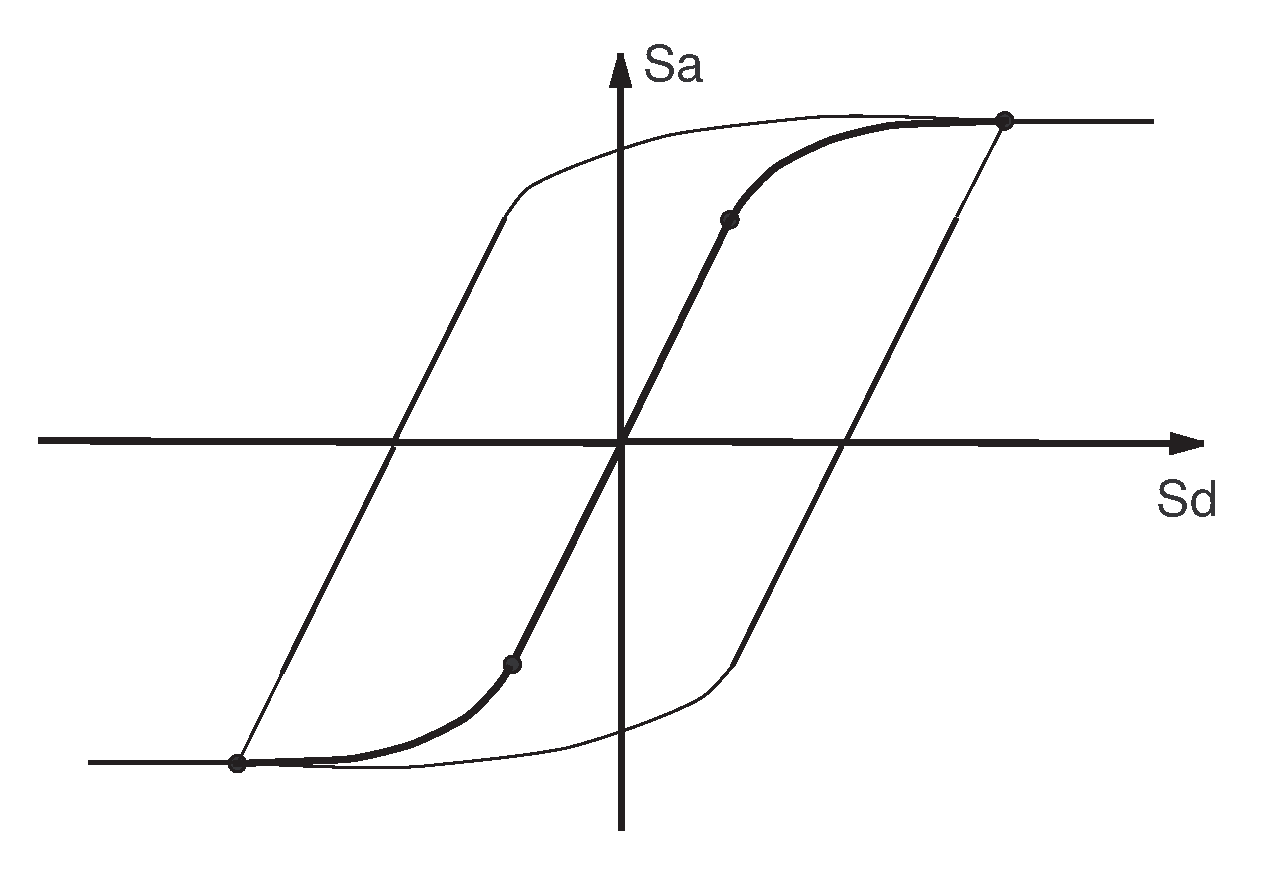
\includegraphics[width=0.4\textwidth]{fig-vdamage-hyst}
\caption{Hysteresis area.}
\label{fig:vdamage-hystarea}.
\end{figure}

Recall that the curved part of the hysteresis boundary is
approximated by
$$
 y = ae^{-bx}+c,
$$
where
$$
 c = A_u, \qquad
 b = \frac{k}{A_u-A_y}, \qquad
 a = (A_y-A_u)e^{b D_y}, \qquad
$$
and the slope of the elastic part is,
$$
 k = \frac{A_y}{D_y}.
$$

The area is calculated by subdividing into three separate areas
(see \fref{fig:vdamage-hyst3})
$$
 A_H = 2(A_1-A_2+A_3).
$$

\begin{figure}[htp]
\centering
\psfrag{A1}{$A_1$}
\psfrag{A2}{$A_2$}
\psfrag{A3}{$A_3$}
\psfrag{Sa}{$S_a$}
\psfrag{Sd}{$S_d$}
\includegraphics[height=0.3\textheight]{fig-vdamage-hyst3}
\caption{Diagram showing the sub-areas used for the hysteresis
area calculation.}
\label{fig:vdamage-hyst3}
\end{figure}


We also define the coordinates (see \fref{fig:vdamage-hyst2})
$$
x_2 = D-\frac{A}{k}, \qquad x_1 = 2x_2+\frac{y_1}{k}, \qquad y_1 =
A_u-A_y.
$$

\begin{figure}[htp]
\centering \psfrag{x1}{$x_1$} \psfrag{x2}{$x_2$} \psfrag{x3}{}
\psfrag{Sa}{$S_a$} \psfrag{Sd}{$S_d$} \psfrag{point}{$(D_u,A_u)$}
\psfrag{Ay}{$A_y$}
\includegraphics[height=0.3\textheight]{fig-vdamage-hyst2}
\caption{Coordinates used for hysteresis area calculation.}
\label{fig:vdamage-hyst2}
\end{figure}

The sub-areas are calculated as
\begin{align*}
 A_1 &= cx_1+\frac{a}{b}(1-e^{-bx_1})\\
 A_2 &= \frac{y_1^2}{2k}\\
 A_3 &= 2A_y(D-D_y).
\end{align*}

Currently the EQRM calculates
hysteretic damping for all events including those in the elastic
region (where the hysteretic damping is zero), because the
calculations are vectorised. Furthermore the code iterates until
the most nonlinear event has converged or the maximum iteration
limit is reached. Some efficiencies might be gained by first
filtering out those events in the elastic region, and then later
filtering out those events which have converged.

Tables of the hysteretic damping coefficients $\kappa_L$,
$\kappa_M$ and $\kappa_L$ are given in \aref{app:buildingpars}.
\tref{tab:vdam-bfactors-damping} provides the hysteretic damping
coefficients $\kappa_L$, $\kappa_M$ and $\kappa_L$ corresponding
to parameters used in the Newcastle and Lake Macquarie study
\citep{dr_Fulford02a}.



\subsection{Finding the intersection point}

The algorithm used to find the intersection point of the suitably
damped demand curve\index{demand curve} with the building capacity
curve\index{capacity curve} is quite simple. However, it is
vectorised over all the synthetic earthquakes. The intersection
point is generally not found exactly, rather it is approximated.

The algorithm can be summarised, as follows:
\begin{enumerate}
\item Locate points on demand curve\index{demand curve} and
building capacity curve\index{capacity curve} which bound the
intersection point, as shown in \fref{fig:vdamage-intersection}.
\item Use linear interpolation to find a first approximation to
the
  intersection point.
\item Use a vertical step to force the intersection to lie on the
  building capacity curve\index{capacity curve}.
\end{enumerate}


\begin{figure}[htp]
\centering
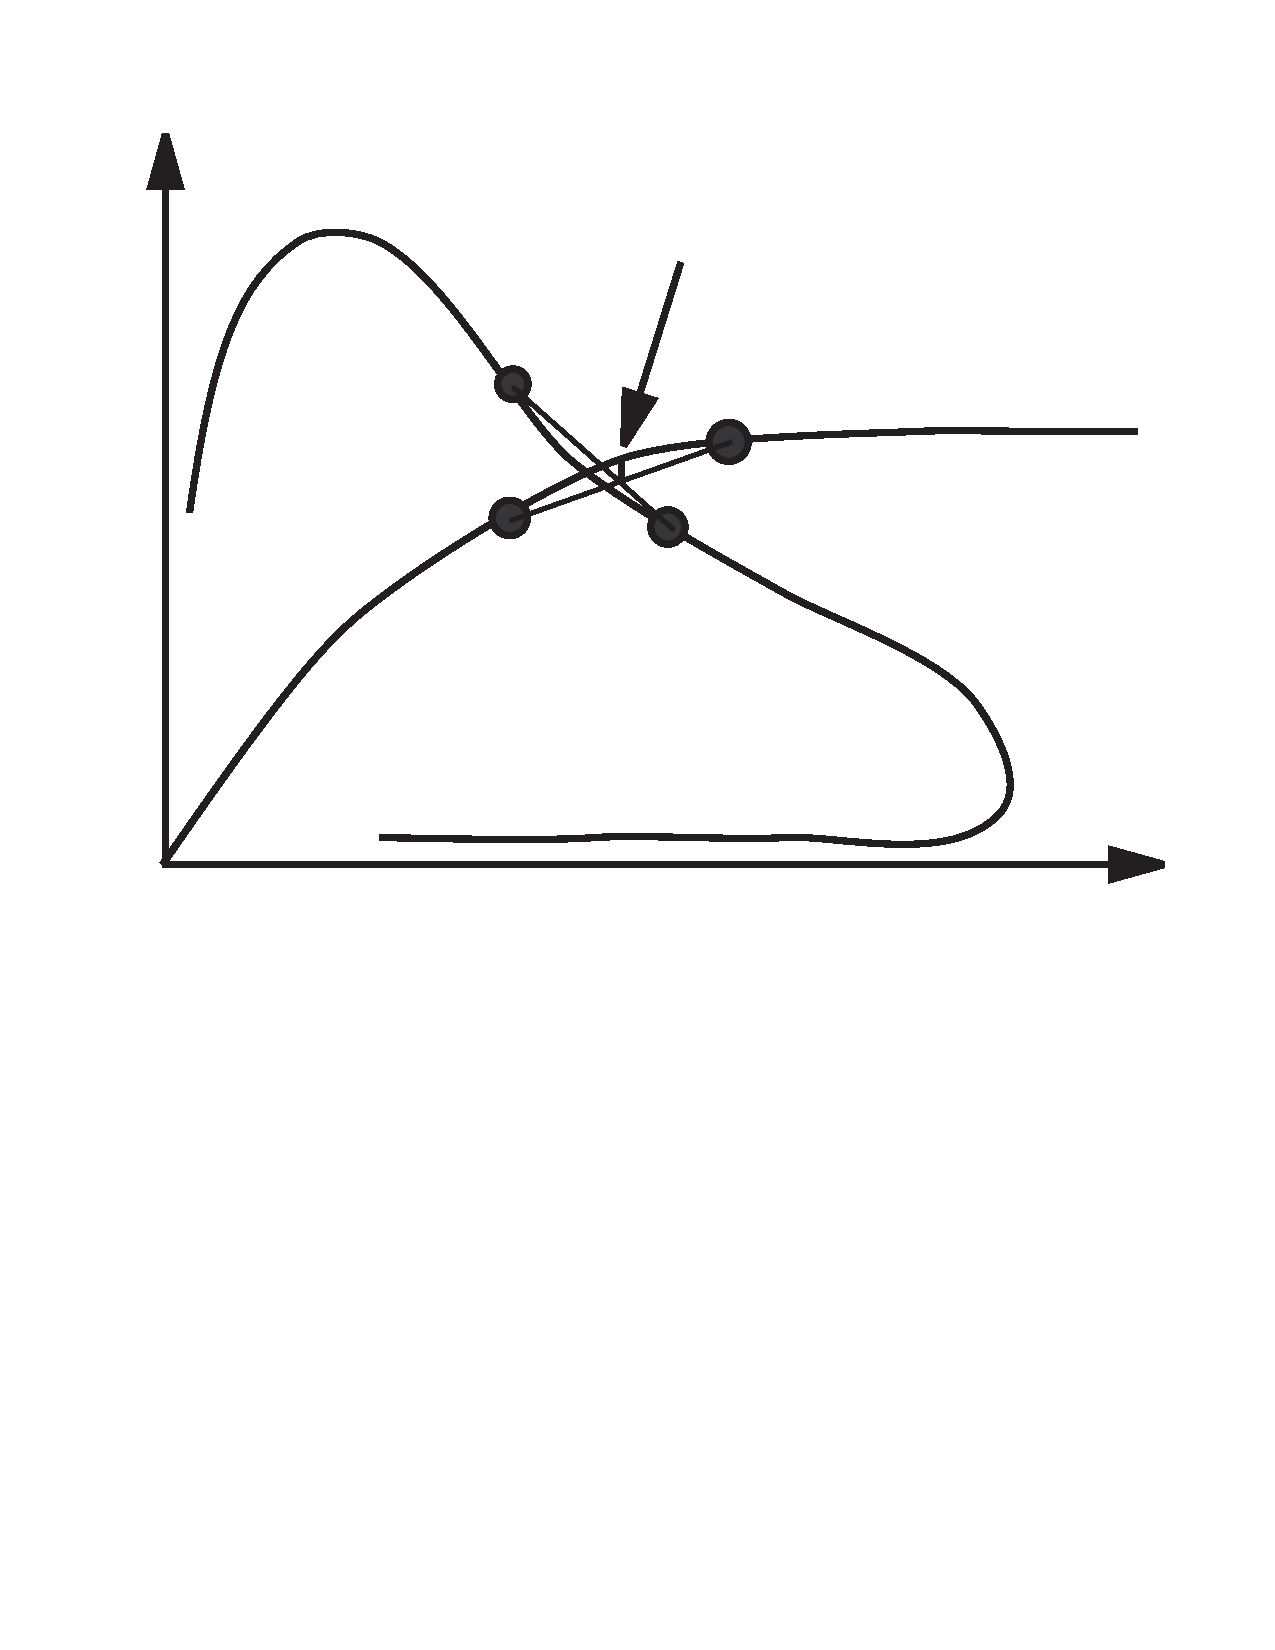
\includegraphics[height=0.3\textheight]{fig-vdamage-intersect}
\caption{Illustration of the algorithm used to approximate the
intersection point of the demand SA curve and the building
capacity curve\index{capacity curve}.}
\label{fig:vdamage-intersection}
\end{figure}

It is important that the approximation to the intersection point
lies on the building capacity curve\index{capacity curve} for the
calculation of of the hysteretic area.

Further refinements could be made to improve the accuracy of the
location of the intersection point. These might involve iterative
procedures which use the tangent of the capacity
curve\index{capacity curve} intersecting the line between the two
points on the demand curve\index{demand curve}, to iteratively
spiral into the true intersection point. However, a more
sophisticated scheme, such as this, may be difficult to code since
it would have to account for all possible variations in the form
of the demand curve\index{demand curve} (after soil amplification
and damping) and might not always converge. Therefore further
refinements are probably not warranted since the current scheme
appears to be sufficiently accurate.






%%%%%%%%%%%%%%%%%%%%%%%%%%%%%%%%%%%%%%%%%%%%%%%%%%%%%%%%%%%%%%%%%%%%%%%%%%%%%
\section{Fragility curves}

Fragility curves give the cumulative probability of a particular
building being in or exceeding a given damage state given  a
seismic demand parameter, such as building peak
displacement\index{peak displacement} or acceleration. There are
separate fragility curve\index{fragility curves}s for each of the
4 cumulative damage states: Slight, Moderate, Extensive and
Complete and the 3 types of damage: (a) Structural Damage (based
on peak displacement\index{peak displacement}), (b) Non-structural
damage-drift sensitive (also based on peak displacement\index{peak
displacement}) and (c) Non-structural damage-acceleration
sensitive (based on peak acceleration\index{peak acceleration}).

\citet[page 5-12, Table 5.2]{dr_FEMA99b} provides a table showing
typical non-structural components of buildings as drift sensitive
or acceleration sensitive. \citet[page 5-13 to 5-23]{dr_FEMA99b}
also provide qualitative descriptions of what the damage states
for structural and non-structural damage correspond to. For
example \textit{slight structural damage} for wood framed
construction corresponds to small cracks in door and window
openings and \textit{complete structural damage} corresponds to an
immediate danger of structure collapse.

In \citet[pages 5-19]{dr_FEMA99b} it is stated that non-structural
(acceleration sensitive) damage to components at or near ground
level may be better characterised by peak ground acceleration
(PGA) rather than peak spectral acceleration $S^*_a$. To this end,
HAZUS suggests a combined use of PGA and $S^*_a$ to model damage
for near ground components. Currently the EQRM considers only
$S^*_a$ when computing damage, however the HAZUS suggestion could
easily be incorporated into future version of the EQRM.


\subsection{Form of fragility curve\index{fragility curves}s}

Each fragility curve\index{fragility curves} is determined by two
parameters: the threshold value of displacement (or acceleration)
and a variability parameter. The form of the fragility
curve\index{fragility curves} is a cumulative log-normal
distribution,
\begin{equation}
\label{eq:vdamage-frag} F(s_{dam} \Vert \bar S^*,\epsilon) =
\ln\left[\Phi\left(\frac{S^*}{\bar S^*}; \epsilon\right)\right]
\end{equation}
where $s_{dam}$ refers to the damage state of interest, $\Phi$ is
the standard cumulative normal distribution function,
$$
 \Phi(x) = \frac{1}{\sqrt{2\pi}}\int_{-\infty}^x e^{-t^2}\,dt,
$$
$S^*$ denotes either peak spectral displacement\index{response
spectral displacement}, $S_d^*$ or peak spectral acceleration,
$S_a^*$, $\bar S^*$ is the median damage state threshold value of
$S^*$ and $\epsilon$ is a variability parameter.

The value $\epsilon$ represents the uncertainty of the damage
state. It is the square root of the variance of the logarithm of
the data (i.e. the log-standard deviation). A zero value for
$\epsilon$ means the the curve approximates a step function, and
so below the threshold value the building is not in the given
damage state and above the threshold it is definitely in the
damage state. The larger the value of $\epsilon$ the more spread
out the curve is, reflecting our less certain knowledge of what
state the building is in (\fref{fig:dam-fragility-var-dstate}).


\begin{figure}[htp]
\label{fig:dam-fragility-var-dstate} \centering
\psfrag{Pr}{$F(s_{dam} \Vert \bar S^*,\epsilon)$}
\psfrag{Sd}{$S^*$} \psfrag{ST}{$\bar S^*$}
\includegraphics[height=0.3\textheight]{fig-vdamage-frag}
\caption{A typical fragility curve\index{fragility curves}, giving
the cumulative probability of
  being in or exceeding
  a certain damage state as a function of the
 peak displacement\index{peak displacement} (or acceleration).}
\label{fig:vdamage-frag}
\end{figure}

\subsection{Damage state thresholds}

The damage state thresholds are the median values that determine the
damage states.

For structural damage and non-structural drift-sensitive damage
the damage state thresholds are determined from provided drift
ratios for each building construction type. For non-structural
acceleration-sensitive damage the damage state thresholds are
obtained from specified acceleration thresholds. For example

\begin{equation}
\label{eq:damage-dstate}
 S_T = \alpha_2 h\delta
\end{equation}

is used to compute the median damage state threshold for
structural damage, where $\delta$ is the drift ratio, $h$ is the
provided height of the building for the given building
construction type and $\alpha_2$ is a building construction
parameter corresponding to the fraction of the building height
(roof) at the location of push-over mode displacement. The
parameters $\alpha_2$ and $h$ are given in
\tref{tab:vdam-building-parameters}. Note that $h$ is given in
feet, however, in the code this is converted into $mm$ (since
$S_d$ is considered throughout the code in $mm$). Tables of drift
ratios, and acceleration values, for different sets of building
parameters are given in the \aref{app:buildingpars}.


\subsection{Variability of the damage states}

The uncertainty of a building being in a given damage state for a
given peak displacement\index{peak displacement}, is characterised
by the variability parameter $\epsilon$ in equation
\eref{eq:vdamage-frag}. As this uncertainty becomes smaller, the
fragility curve\index{fragility curves} steepens and becomes more
like a step function, as shown in \fref{fig:vdamage-frag-var}.

\begin{figure}[htp]
\centering \psfrag{vert}{$F(s_{dam} \Vert \bar S^*,\epsilon)$}
\psfrag{hor}{$S^*$}
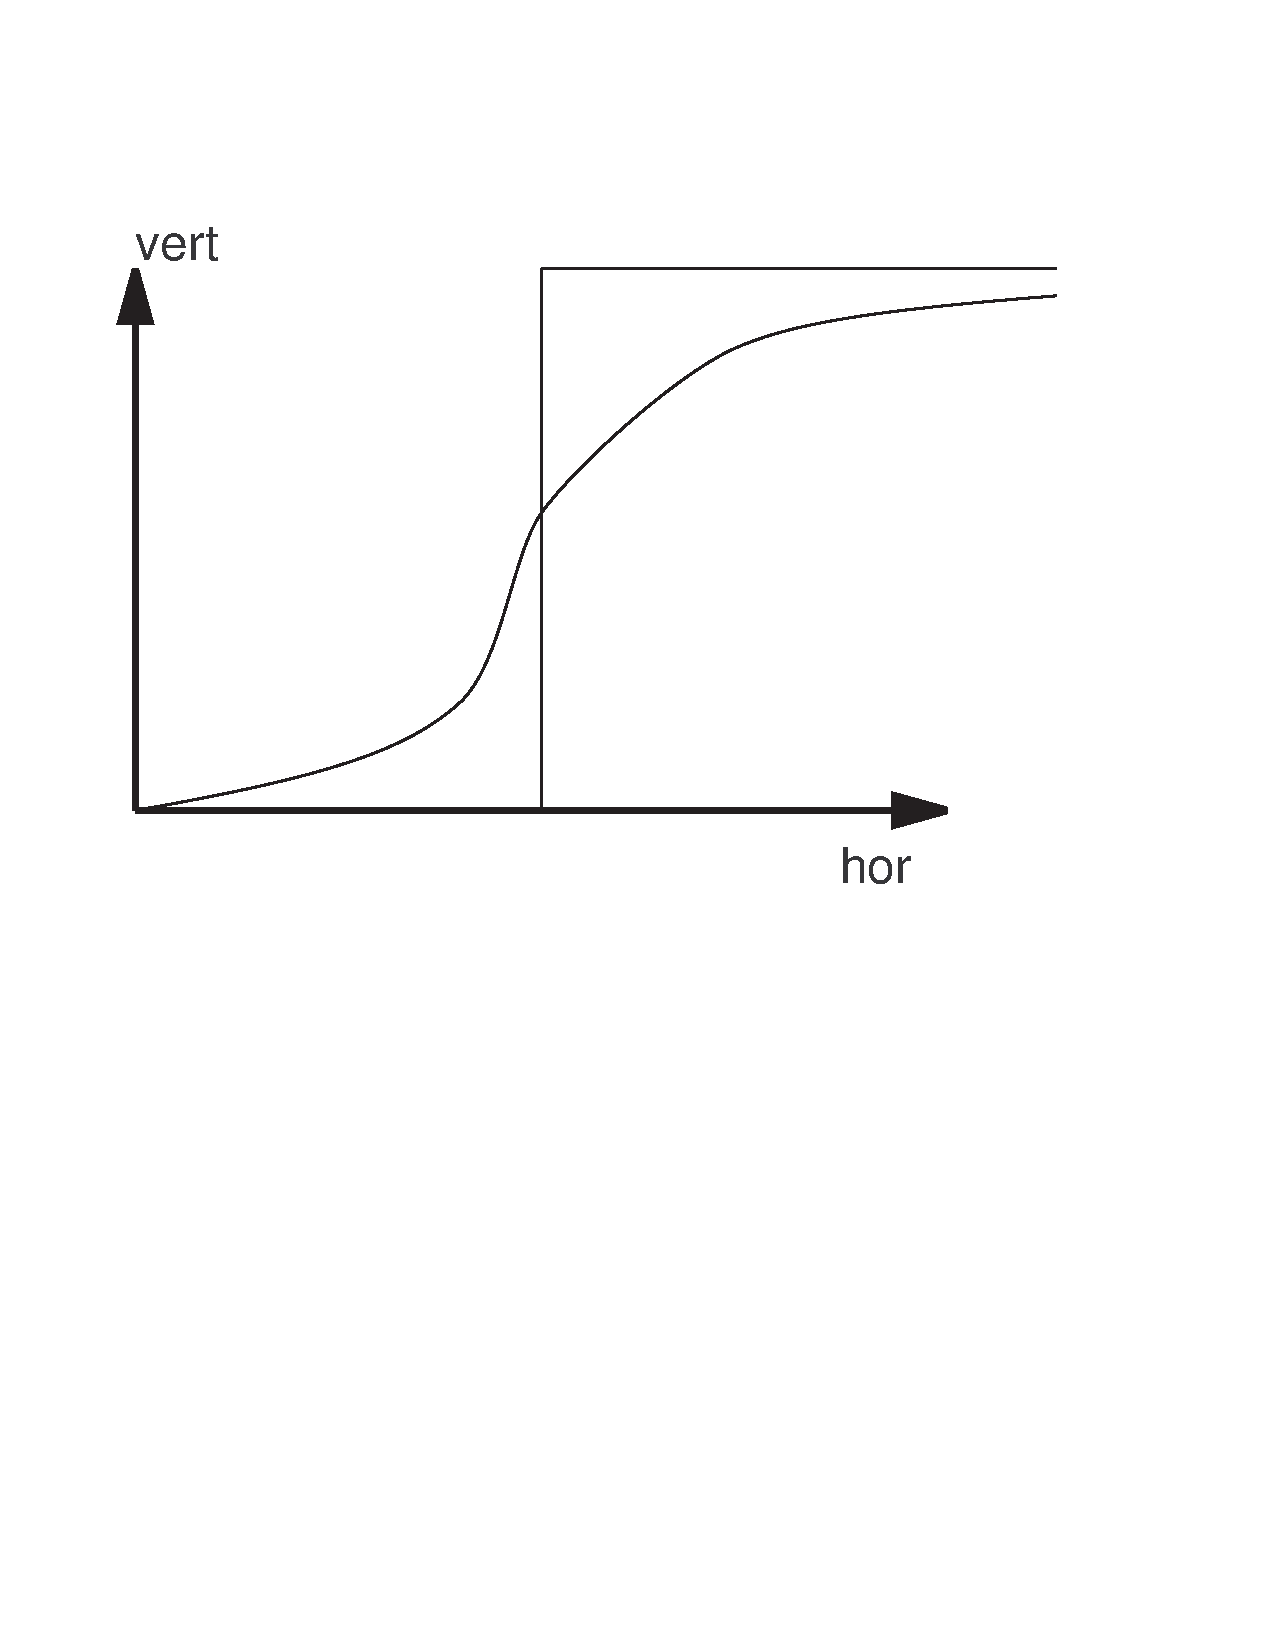
\includegraphics[height=0.3\textheight]{fig-vdamage-frag-step}
\caption{As the variability of a fragility curve\index{fragility
curves} is reduced the
  fragility curve\index{fragility curves} steepens and becomes more like a step function.}
\label{fig:vdamage-frag-var}
\end{figure}


We follow \cite{dr_FEMA99b} in setting
\begin{itemize}
\item for structural damage $\epsilon=0.4$, \item for
non-structural, drift sensitive damage $\epsilon=0.5$, \item for
non-structural, acceleration sensitive damage,
  $\epsilon=0.6$.
\end{itemize}
Note that HAZUS does not give any references to the derivation of
these values.


\subsection{Incremental probabilities}

The fragility curve\index{fragility curves}s give the probability
of being in the given damage state or lower. That is, they are
cumulative probabilities. For our Monte Carlo simulation approach
we need the incremental probabilities of the building being in the
given damage state. For example,  suppose we have the fragility
curve\index{fragility curves} for the extensive damage state,
$\Pr(d \le E)$. To find $\Pr(d=E)$, we calculate
$$
\Pr(d=E) = \Pr(d\le E) - \Pr(d\le M).
$$
This is illustrated in \fref{fig:vdamage-frag-inc}.

\begin{figure}[htp]
\centering
\psfrag{Sd}{$S^*$}
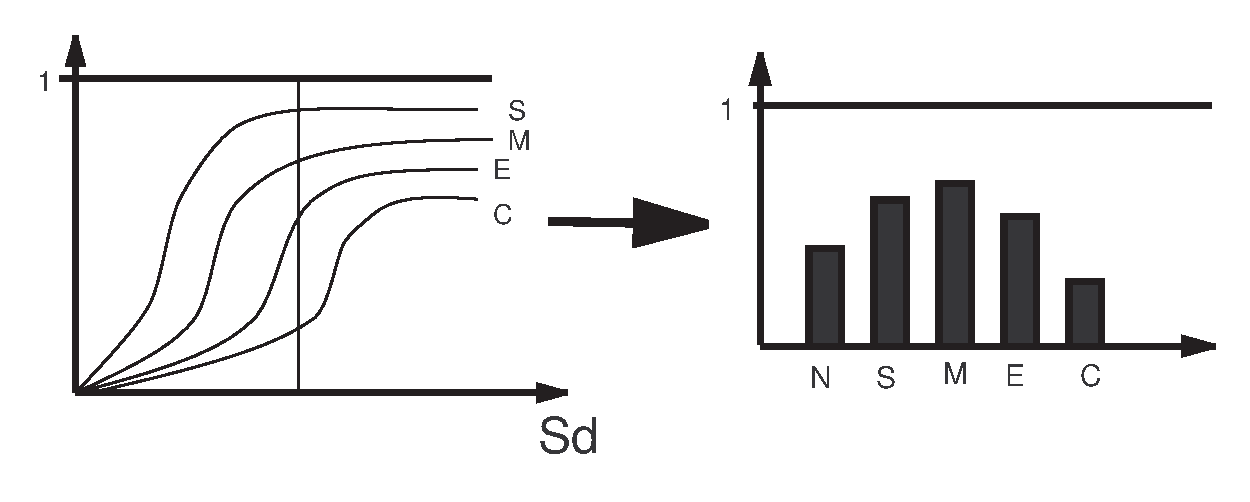
\includegraphics[width=0.95\textwidth]{fig-vdamage-frag-inc}
\caption{Converting the cumulative
  probabilities in the fragility curves\index{fragility curves} to incremental probabilities
  describing the probability that the building component is in a given damage state.}
\label{fig:vdamage-frag-inc}
\end{figure}


\section{Differences from HAZUS methodology}


A key difference in our implementation of the Capacity Spectrum
Method\index{capacity spectrum method} to that used by HAZUS is
using the full response spectrum for intersecting with the
building capacity curve\index{capacity curve} rather than a design
spectra based on only a few building periods. For example, the
HAZUS approach only uses periods 0.3 and 1.0 seconds. Our approach
has the advantage that the full structure of the response spectrum
and all the available information for the soils amplification
factors, at all periods, is taken into account rather than at only
two periods (\creftwo{ch:atten}{ch:reg}). There are also some
minor differences in the way that demand curve damping is applied.

Another difference is in how the fragility curve\index{fragility
curves}s are used. In HAZUS, the fragility curve\index{fragility
curves}s incorporate not only the variability of the damage state
thresholds, but also the variability of the capacity
curve\index{capacity curve} and the ground-shaking. A `convolution
procedure', as described in \cite{dr_Kircher97b}, is used to
convolve the various log-normal probability distributions for
ground-shaking and building capacity curve\index{capacity curve}
by calculating intersection points for a range of randomly
selected demand and capacity curve\index{capacity curve}s, then
fitting a log-normal distribution. In the EQRM the fragility
curve\index{fragility curves}s includes only the variability for
being in the given damage state and not the variability associated
with ground shaking or building type\index{building type}. The
variability associated with the fragility curve\index{fragility
curves} is defined by a cumulative log-normal distribution with
variability parameters $0.4$, $0.5$ and $0.6$ for structural
damage, non-structural damage (drift sensitive) and non-structural
damage (acceleration sensitive), respectively. The variability
associated with ground shaking
(\sreftwo{attn:uncertainty}{sec:regolith-incorp-unc}) and building
type (\sref{sec:dam-capacity-var}) are incorporated elsewhere in
the Monte-Carlo simulation.

\subsection{Extra features}

The risk component of the EQRM also has a number of extra features
or alternative operation modes that are not offered by the HAZUS
methodology. Two of the more significant extra features are:
\begin{enumerate}
\item The use of \textbf{uniform hazard spectra} instead of demand
curve\index{demand curve}s. This effectively drives the risk
calculation by hazard values rather than individual earthquakes.
The process is discussed further in \citet{dr_Patchett04a}. 
\item The use of \textbf{Modified Mercali Intensity (MMI) damage
curves} rather than the capacity spectrum method\index{capacity
spectrum method}. The EQRM has the capability to use an MMI
attenuation model (currently only Gaull is coded) and will compute
risk using in-built damage curves that relate percentage damage to
MMI. Note that the damage curves are exponential in shape and that
the percentage damage estimates represent damage to the entire
structure rather than components of the structure.
\cite{dr_Edwards04a} provide an example of the use of damage
curves with the EQRM.
\end{enumerate}


\chapter{Losses}
\label{ch:losses}

\section{Overview}
The EQRM considers two types of loss:
\begin{enumerate}
\item \textbf{direct financial loss} defined as the cost involved
in replacing damaged building components and/or contents; and
\item \textbf{social loss} defined as the number (or probability)
of casualties and injuries as a result of a simulated scenario.
\end{enumerate}
This chapter describes the direct financial and social loss
modules.

\section{Direct financial loss}

\subsection{General financial loss equations: loss for a single building}

Recall that the capacity spectrum method\index{capacity spectrum
method} assumes that each building comprises three main
components, namely a structural, non-structural drift sensitive
and non-structural acceleration sensitive component.
\sref{ch:damage} described how the damage experienced by each
building is computed separately for each of the components. It is
therefore necessary to partition the replacement cost of the
building into the replacement cost for each of the three
components. The proportion chosen for each building component is a
function of the buildings construction and usage type as well as
the usage classification system. For example
\tref{tab:grids-costproportions} illustrates the proportion of the
replacement value corresponding to a couple of different buildings
for both the HAZUS\index{building usgage!HAZUS} and
FCB\index{building usgage!FCB} classification system. The
\typeself{set}{da}{ta} flag \typepar{b\_usage}{\_type}{\_flag} can
be used to select the usage classification system and consequently
the desired cost proportions.

\begin{table}
\centering \caption{Examples of costing splits for the
FCB\index{building usgage!FCB} and HAZUS usage
classification\index{building usgage!HAZUS}.}
\label{tab:grids-costproportions}  \vspace{0.8em}
\begin{tabular}{|l|l|}

 \hline
\textbf{FCB Usage Classification} &  \\
 & \\
\textit{111 -- W1BVTILE:} & \\
structural & 23.44\%\\
non-structural drift sensitive & 50.00\%\\
non-structural acceleration sensitive & 26.56\%\\
 & \\
\textit{491 -- C1MSOFT:} & \\
structural & 15.32\%\\
non-structural drift sensitive & 34.23\%\\
non-structural acceleration sensitive & 50.45\%\\
\hline
\textbf{HAZUS Usage Classification} &  \\
 & \\
\textit{RES1  -- W1BVTILE:} & \\
structural & 23.44\%\\
non-structural drift sensitive & 50.00\% \\
non-structural acceleration sensitive & 26.56\%\\
 & \\
\textit{COM5 -- URMLMETAL:} & \\
structural & 13.79\%\\
non-structural drift sensitive & 34.48\%\\
non-structural acceleration sensitive & 51.72\%\\
\hline
\end{tabular}
\end{table}

Let $P_{i \alpha}$ denote the probability of being in a damage
state $\alpha=(1,2,3,4)=(S,M,E,C)$ corresponding to Slight,
Moderate, Extensive and Complete damage, where the index
$i=(1,2,3)=(s, n_d, n_a)$ corresponds to the type of damage: drift
sensitive structural damage (s), drift sensitive non-structural
damage ($n_d$) and acceleration sensitive non-structural damage
($n_a$). Contents damage is factored in later.

We also define $L_i$ as the financial loss corresponding to the 3
building components (structural damage, $i=s=1$; drift-sensitive
non-structural damage, $i=n_d=2$; acceleration-sensitive
non-structural damage $i=n_a=3$; and $L_4$ as the financial loss
due to damage of contents.


Let $R_i$ denote the replacement cost component of the building
per unit floor area, for $i=(1,2,3)=(s,n_d,n_a)$. Thus
$R=R_1+R_2+R_3$ is the total replacement cost (per unit floor
area) of the building (excluding contents). The financial loss,
for a single building, excluding contents, is then given as the
weighted sums of the probabilities
\begin{align*}
\label{eq:this-loss}
 L_1 &= C_0\sum_{\alpha=1}^4
   f_{\alpha, 1} R_1 A P_{\alpha, 1} =
   \sum_{\alpha=1}^4 f_{\alpha, 1} g_1R A P_{\alpha, 1},\\
L_2 &= C_0 \sum_{\alpha=1}^4
   f_{\alpha, 2} R_2 A P_{\alpha, 2} =
   \sum_{\alpha=1}^4 f_{\alpha, 2} g_2R A P_{\alpha, 2}, and\\
L_3 &= C_0 \sum_{\alpha=1}^4
   f_{\alpha, 3} R_3 A P_{\alpha, 3} =
    \sum_{\alpha=1}^4 f_{\alpha, 3} g_3R A P_{\alpha, 3},
\end{align*}
where $A$ is the floor area of the building (in $\mathrm{m}^2$).
Note that $R$ is the replacement cost of the building, $f_{\alpha,
i}$ is a repair cost fraction of replacement cost for the given
damage state, $g_i$ is the damage component replacement value as a
fraction of the replacement value, and $C_0$ is a regional cost
factor\index{regional cost factor}. The total loss of the
building, excluding contents, is $L=L_1+L_2+L_3$.

Note that for percentage loss (loss divided by the value of the
building) the quantity $c_0R$ cancels.


For example, the total repair cost for a building (excluding contents)
in damage
state $\alpha=3=E$ is $f_{3,1}R_1+f_{3,2}R_2+f_{3,3}R_3$.
The probabilities $P_{\alpha, i}$ correspond to the probability
of the building component $i=(s, n_d, n_a)$ being in damage state
$\alpha=(S,M,E,C)$.

The regional cost factor\index{regional cost factor}, $C_0$, is a
normalising factor to calibrate the replacement costs if
necessary. For example in the Newcastle risk assessment
\citep{dr_Fulford02a} the HAZUS cost values were used (see
\tref{tab:replace_costs}) and converted to the Newcastle region
using $C_0= 1.4516$. In this particular case the $C_0$ was
computed by assuming that a $100\,\mathrm{m^2}$ brick veneer
residential house (RES1, W1BVTILE) had a replacement cost of
AUS\$1,000 per $\mathrm{m}^2$ (this value of \$1000 having been
obtained from NRMA web site for the NSW region). In other studies,
such as the Perth Cities case study, the replacement costs (see
\tref{tab:grids-bdatabasecolumns}) were defined for the region and
no further correction was required. Note that the parameter $C_0$
is \typepar{c}{}{i} in the \typeself{set}{da}{ta} file.

\begin{table}[p]
\centering \caption{Calculated replacement costs (AUD
$\mathrm{m^2}$) of building
  usage types.}
  \vspace{0.8em}
\label{tab:replace_costs} \small
\input tab-v-losses-repcosts
\end{table}


The repair cost factors $f_{\alpha, i}$
are the proportions of the replacement costs (for each building
component $i=(1,2,3)=(s, n_d, n_a)$  per floor area.
For structural damage,
\begin{equation}
 f_{\alpha, 1} = (2\%, 10\%, 50\%, 100\%),
\end{equation}
for non-structural damage (drift-sensitive),
\begin{equation}
 f_{\alpha, 2} = (2\%, 10\%, 50\%, 100\%),
\end{equation}
and for non-structural damage (acceleration-sensitive)
\begin{equation}
 f_{\alpha, 3} = (2\%, 10\%, 30\%, 100\%),
\end{equation}
These values are taken from \cite{dr_FEMA99b}. For example, the
repair cost for the acceleration-sensitive components in the
extensive damage state are given by the product $f_{33}R_3$, so
that if the replacement cost for complete damage is \$500 per
square metre, the repair cost would be $30/100\times\$500$.


The directory \typedir{*/eqrm}{/datacvt}{/econsoclosspars}
contains tools to assist the preparation of direct financial loss
parameters. The files
\typeparfile{RcPerWrt}{BuildCFCB}{usageEdwards}{.xls} and
\typeparfile{RcPerWrt}{BuildCHazus}{usageEdwards}{.xls} contain
the replacement cost component of the building per unit floor area
$R_i$ for the FCB\index{building usgage!FCB} and
HAZUS\index{building usgage!HAZUS} usage types respectively. The
MATLAB function \typefunc{per\_replace}{\_cost\_wrt}{\_bc\_usage}
converts these excel files to \texttt{*.MAT} that can be used by
the EQRM. The EQRM assumes the replacement cost components to be
independent of the construction type. There are a few exceptions,
which have not been implemented. These are based on the tables
given in \cite{dr_FEMA99b}, in particular, Table 25.2a (page
15-12), Table 13.3 (page 15-14) and Table 15.4 (page 15-15). In
principle the tools in
\typedir{*/eqrm}{/datacvt}{/econsoclosspars} allow the replacement
cost components to be a function of both usage and construction
type. Note that \typefunc{per\_replace}{\_cost\_wrt}{\_bc\_usage}
attributes proportions of the building's total value to its
different components. Recall form
\tref{tab:grids-bdatabasecolumns} that the replacement costs for
each building is stored with the building database.

The contents damage, $L_4$, is based only on the probabilities for
acceleration sensitive non-structural damage being in Slight,
Moderate, Extensive or Complete states, and on the total contents
repair costs $R_4$ defined by the building database\index{building
database} (see \tref{tab:grids-bdatabasecolumns}). The cost $L_4$
is then added to the building damage cost $L$ to get the overall
loss $L^*$ which includes contents.

As with the building components, the loss for contents damage, is
expressed as a weighted sum of probabilities of the acceleration
sensitive components for each damage state,
\begin{equation}
\label{eq:vlosses-contents}
 L_{4} = C_0 \sum_{\alpha=1}^{4} f_{\alpha,4}R_4P_{\alpha 3},
\end{equation}
where $P_{\alpha 3}$ is the probability of the acceleration
sensitive component of the building being in damage state
$\alpha=(1,2,3,4)=(S,M,E,C)$ and $f_{\alpha,4}$ is the repair cost
fraction of the replacement value for the contents in damage state
$\alpha=(S,M,E,C)$. This factor is expressed as a percentage in
\tref{tab:replace_costs} and has been taken from \citet[Table
15.6, page 15-21]{dr_FEMA99b}. Furthermore, for contents damage,
\begin{equation}
 f_{\alpha 4} = (1\%, 5\%, 25\%, 50\%).
\end{equation}
These values assume that 50\%\ of the contents in complete damage
can be salvaged with similar proportions for lesser damage
\citep{dr_FEMA99b}. If the \typeself{set}{da}{ta} parameter
$\typepar{aus}{\_contents}{\_flag}$ is set to 1 the following
modifications are made as to suggested by George Walker (Aon Re):
\begin{enumerate}
\item HAZUS usage\index{building usgage!HAZUS} only: The contents
value of usage types 1 to 10, 24 and 29 (see
\tref{tab:grids-HAZUSusage}) are re-assigned to 60\% of $R_4$.
\item $f_{\alpha 4}$ is re-assigned to $(2\%, 10\%, 50\%, 100\%)$
which assumes that no contents will be salvaged from complete
damage of Australian buildings.
\end{enumerate}

\subsection{Aggregated loss and survey factors}
\label{sec:loss-surveyfacts}

Each building in the database represents a sample from its
surrounding area. There is a building survey factor associated
with each building, which represents the additional number of
buildings that are represented by the modelled building (see
\tref{tab:grids-bdatabasecolumns}). Typically the extra buildings
are of the same type and are located in close proximity to the
modelled building.

The aggregated loss is therefore the weighted sum of the losses of
each building in the database with its corresponding survey factor.

The aggregated financial loss values are saved to a file of form
\typeoutput{<site\_loc>}{\_db\_save}{decloss}{.mat}. If the
\typeself{set}{da}{ta} parameter
$\typepar{save}{\_ecloss}{\_flag}=1$ a combined loss for the
building and contents is saved; whereas if
$\typepar{save}{\_ecloss}{\_flag}=2$ the losses for the building
and contents are saved separately.


\subsection{Cutoff values}

The damage and financial loss models estimate small (but finite)
damage for very small ground accelerations. This arises due to the
asymptotic nature of the fragility curves. A cutoff value has been
implemented in the code to prevent such small values being
calculated. The cutoff is in terms of PGA and is controlled by the
\typeself{set}{da}{ta} parameter \typepar{pga}{\_min}{damage}. For
all those events having peak ground acceleration (pga) values
smaller than \typepar{pga}{\_min}{damage} at the building
location, the financial loss is set to zero. Typically it is
assumed that no damage worth reporting occurs for ground
accelerations smaller than $\typepar{pga}{\_min}{damage}=0.05g$.


\section{Social losses}

The EQRM includes a module for computing the injuries and
casualties associated with a scenario simulation (see
\sref{sec:source-scenario}). The code for considering social
losses associated with probabilistic simulations has not yet been
written. The social loss module is activated by setting the
\typeself{set}{da}{ta} parameter \typepar{save}{\_socloss}{\_flag}
to 1. When activated, the social loss module produces a file
\typeoutput{<site\_loc>}{\_db\_save}{dsocloss}{.mat} that can be
processed by the MATLAB script \typescript{newc}{89plot}{histsoc}.

For the Newcastle 1989 simulation the results are slightly greater
than those observed in the actual earthquake (e.g. median of 45
casualties vs 13 casualties actually recorded). Further
investigation of the model is recommended before it is widely
used. Firstly, a check on the accuracy of the distribution of the
population would be useful. Secondly, some thought should be given
to a model which distributes the population randomly. It is
expected that this will result in a greater spread of the
distribution of injuries.

Chapter 13 of \cite{dr_FEMA99b} provides a detailed description of
the methodology behind social loss calculations.

\section{Key functions, flags and parameters}

\begin{tabular}{llp{0.5\textwidth}}
\hline
\textbf{Name} & \textbf{Type} & \textbf{Description} \\
\hline
\splitrowdir{*/eqrm/datacvt}{/econsoclosspars} & Dir & Tools to assist the preparation of direct financial loss parameters.\\
\keyrowsep \splitrowfunc{per\_replace\_cost}{\_wrt\_bc\_usage} & Function & Converts the \typeparfile{RcPerWrt}{BuildCFCB}{usageEdwards}{.xls} and \typeparfile{RcPerWrt}{BuildCHazus}{usageEdwards}{.xls} to the required format for the EQRM.\\
\keyrowsep \typefunc{so}{c}{loss} & Function & Function for calculating injury probabilities.\\
\keyrowsep \typescript{newc}{89plot}{histsoc} & Script & MATLAB script to plot injury probabilities (for Newcastle scenario only).\\
\keyrowsep \splitrowparfile{RcPerWrtBuildCFCB}{usageEdwards}{.xls} & Par File & Replacement cost component of the building per unit floor area for the HAZUS usage classification.\\
\keyrowsep \splitrowparfile{RcPerWrtBuildCHazus}{usageEdwards}{.xls}  & Par File & Replacement cost component of the building per unit floor area for the FCB usage classification.\\
\keyrowsep \typepar{c}{}{i} & Par & Regional cost index multiplier.\\
\keyrowsep \typepar{aus}{\_contents}{\_flag} & Par & Contents value for residential buildings and salvageability after complete building damage.\\
\keyrowsep \typepar{pga}{\_min}{damage} & Par & minimum PGA(g) below which financial loss is assigned to zero.\\
\keyrowsep \typepar{save}{\_ecloss}{\_flag} & Par & Options for saving direct financial loss data.\\
\keyrowsep \typepar{save}{\_socloss}{\_flag} & Par & Options for saving casualty and injury data.\\
\keyrowsep \splitrowoutput{<site\_loc>\_db}{\_savedecloss}{.mat} & Output & Output file containing the loss estimates for an EQRM risk simulation.\\
\hline
\end{tabular}

\chapter{Hazard and risk results}
\label{ch:risk}


\section{Overview}

Earlier chapters have described how to generate synthetic
earthquakes, propagate (or attenuate) the response spectral
acceleration\index{response spectral acceleration} and compute
loss. This chapter describes how to `aggregate' the above
information to estimate earthquake hazard and earthquake risk. A
number of diagrams are used to demonstrate the common techniques
for visualising earthquake hazard and risk.

\section{Calculating hazard and risk}

Consider a random variable $Y$ such that; \begin{itemize} \item
$Y$ refers to the response spectral acceleration\index{response
spectral acceleration} $S_a$ at a particular site in the case of
hazard, or \item $Y$ indicates the loss, either at a particular
simplicity we will assume that $Y$ represents the aggregated loss
as a percentage of building stock value.
\end{itemize}

A common way to represent $Y$ is in terms of a probability of
exceedance in one one year. To achieve this we assume that
earthquakes occur as a Poisson process \citep{dr_McGuire90a}. This
means that the earthquake process has no memory; or in other
words, the probability of an earthquake today does not depend on
whether or not an earthquake occurred yesterday. Mathematically,
this assumption can be represented as follows:
\begin{equation}
 \Pr(T, Y\ge y) = 1 - e^{\lambda_Y(y)t},
\end{equation}
where t is a time interval in years (typically 1 year) and
$\lambda_Y(y)$ is the annual exceedance rate. The return period is
given by \eref{eq:risk-rptolambda}:
\begin{equation}
\label{eq:risk-rptolambda} R_Y(y) = \frac{1}{\lambda_Y(y)}.
\end{equation}

\subsection{Computing the annual exceedance rate}
\label{sec:risk-ann-exceed-rate}

\cref{ch:source} described the Monte-Carlo approach used to
generate earthquakes. \crefmulti{ch:atten}{ch:losses} describe how
to compute an $S_a$ or loss value for each of the synthetic
events. It follows, therefore that there exists a set of $N_s$
numbers $\{Y_i\}_{i=1}^{N_s}$ with corresponding event activities
$\{r_{\nu _i}\}_{i=1}^{N_s}$ (see \sref{sec:magnitude_selection}),
where $N_s$ is the number of simulated events\index{simulated
event}.

The annual exceedance rate $\lambda_Y(y)$ is computed from the
event activity through the following process:
\begin{enumerate}
\item re-order the values $\{Y_i\}_{i=1}^n$ from largest to
smallest and re-order the corresponding event activities such that
the $Y_i-r_{\nu _i}$ pairs are not separated.
\begin{equation}
\label{eq:eva-vectors1} \left[\begin{matrix}
  y_{1}\\ y_{2} \\ \vdots\\ y_{n}
\end{matrix}\right],
\ \left[\begin{matrix}
 r_{\nu_1} \\ r_{\nu_2} \\ \vdots\\ r_{\nu_n}
\end{matrix}\right]
\to \left[\begin{matrix}
  y_{1^*}\\ y_{2^*} \\ \vdots\\ y_{n^*}
\end{matrix}\right],
\ \left[\begin{matrix}
 r_{\nu_1^*} \\ r_{\nu_2^*} \\ \vdots\\ r_{\nu_n^*}
\end{matrix}\right]
\end{equation}
\item evaluate $\lambda_Y(y)$ by computing the cumulative sum of
event activities.
\begin{equation}
\label{eq:eva-vectors2} \left[\begin{matrix}
 \lambda_{Y_{1^*}}\\ \lambda_{Y_{2^*}} \\ \vdots\\ \lambda_{Y_{n^*}}
\end{matrix}\right] =
\left[\begin{matrix}
  r_{\nu_1^*}\\
   r_{\nu_1^*}+ r_{\nu_2^*} \\
   \vdots\\
   r_{\nu_1^*}+ r_{\nu_2^*} + \ldots + r_{\nu_n^*}\\
\end{matrix}\right],
\end{equation}
\end{enumerate}
The asterisk in \ereftwo{eq:eva-vectors1}{eq:eva-vectors2} refer
to re-ordered values.


\section{Earthquake hazard results}
\label{sec:risk-hzd-results} The EQRM estimates the earthquake
hazard $E_H(R_Y)$ at the return periods $R_Y$ defined in the
\typeself{set}{da}{ta} vector \typepar{rtrn}{\_}{per} by
interpolating the values $\{ \lambda_{Y_i^*}\}_{i=1}^{N_s}$ and
$\{Y_i^*\}_{i=1}^{N_s}$ to the values $1/R_Y$ (see
\eref{eq:risk-rptolambda}). In the case of earthquake hazard the
random variable $Y$ refers to the response spectral
acceleration\index{response spectral acceleration} and is
therefore a function of building period $T_o$. The earthquake
hazard information is saved in the output file
\typeoutput{<site\_loc>}{\_db}{\_hzd}{.mat}. It is important to
emphasise that only the hazard information is saved, the
information for individual synthetic earthquakes is discarded.
This means that the earthquake hazard information can not be
de-aggregated in terms of causative events.

The EQRM offers three tools for visualising the earthquake hazard:
\begin{enumerate}
\item the earthquake hazard map, \item the hazard exceedance
curve, and \item the uniform hazard spectra.
\end{enumerate}

\subsection{Hazard maps}

Earthquake hazard maps can be used to illustrate the earthquake
hazard across a spatial region. The earthquake hazard $E_H(R_Y)$
is plotted for a specific building period $T_o$ and return period
$R_Y$.
\begin{figure}
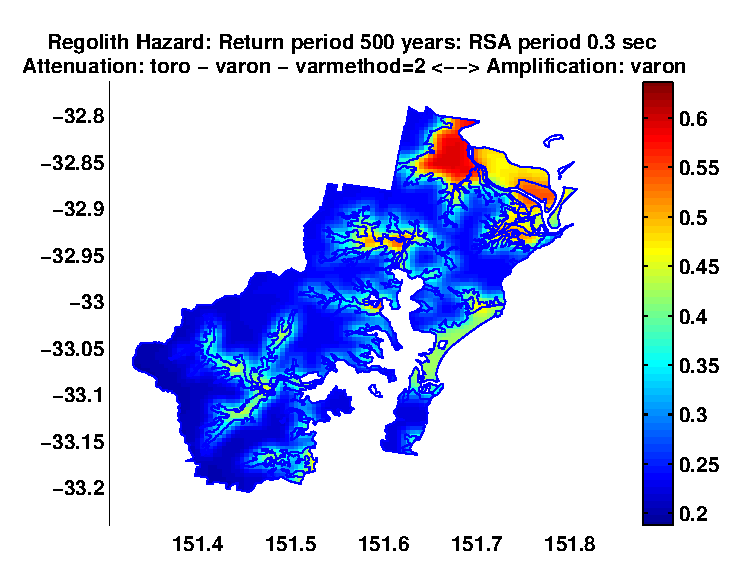
\includegraphics[width=1\textwidth]{fig-risk-hzdmap}
\caption{Newcastle and Lake Macquarie hazard map for return period
of 500 years and $S_a$ period of 0.3 seconds}
\label{fig:risk-hazardmap}
\end{figure}
\fref{fig:risk-hazardmap} provides an example of a hazard map for
the Newcastle and Lake Macquarie region.

It is necessary to draw a number of hazard maps corresponding to
different $T_o$ and $R_Y$ in order to understand the hazard across
a spatial region. Traditionally return periods considered for
building design correspond to a 2\% and/or 10\% probability of
exceedance within 50 years. An exceedance probability of 10\% in
50 years equates to a return period of roughly 500 years and an
exceedance probability of 2\% in 50 years corresponds to roughly
2500 years.

The EQRM post processing tool \typefunc{plot}{\_hzd}{\_map}  can
be used to generate hazard maps. The tool
\typefunc{create}{\_gis}{\_output} can be used to export the data
in \typeoutput{<site\_loc>}{\_db}{\_hzd}{.mat} to a convenient
file for plotting in GIS.

\subsection{Hazard exceedance curves}

The exceedance probability curve for hazard (also known as the
hazard exceedance curve or hazard curve) represents a technique
for visualising the earthquake hazard at a single location. The
hazard exceedance curve expresses $P(Y \ge y)$ at a single
location as a function of the earthquake hazard ($Y = S_a$). Note
that unlike the hazard map, the hazard exceedance curve presents
the hazard corresponding to the `full' range of probability levels
(return periods).
\begin{figure}
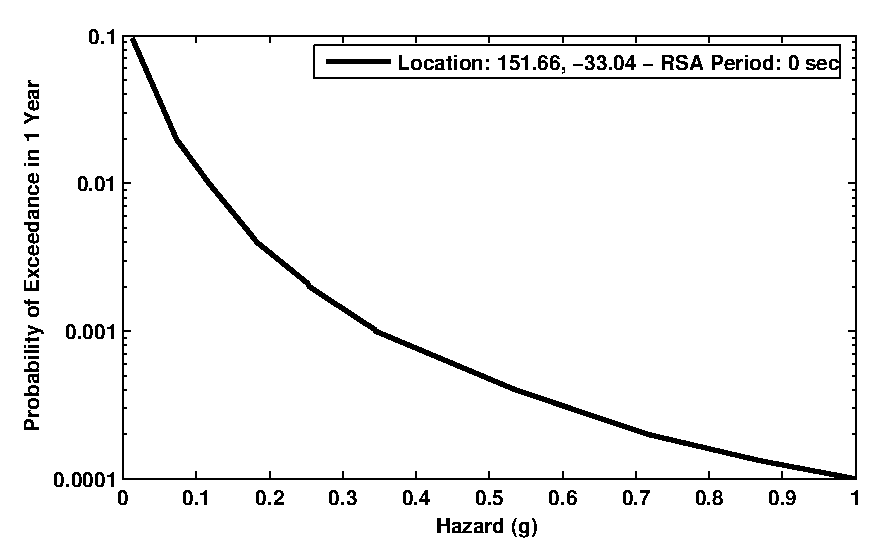
\includegraphics{fig-risk-hzdexceedcurve}
\caption{Peak ground acceleration hazard exceedance curve for the
Newcastle central business district.}
\label{fig:risk-hzdexceedcurve}
\end{figure}
\fref{fig:risk-hzdexceedcurve} provides an example of a hazard
exceedance curve for the Newcastle central business district. The
EQRM post processing tool \typefunc{plot}{\_singlesite}{\_hzd} can
be used to generate hazard exceedance curves.

\subsection{Uniform hazard spectra}

The uniform hazard spectra represents another technique for
visualising the earthquake hazard at a single location. The hazard
for a specified probability level (return period) is plotted for
all $S_a$ periods.
\begin{figure}
\includegraphics{fig-risk-uhs}
\caption{Uniform hazard spectra for return period of 500 years for
a single site on regolith in the Newcastle region.}
\label{fig:risk-hazarduhs}
\end{figure}
\fref{fig:risk-hazarduhs} provides an example of an uniform hazard
spectra for the Newcastle central business district. The EQRM post
processing tool \typefunc{plot}{\_singlesite}{\_hzd} can also be
used to generate uniform hazard spectra.

\section{Earthquake risk results}

The EQRM returns the loss for each earthquake-building pair. This
information is saved in the file
\typeoutput{<site\_loc>}{\_db\_saved}{ecloss}{.mat} along with
other information such as building values, the event activity for
each synthetic earthquake and the distance between the
building-earthquake pair. It is important to note that this
technique for data storage is fundamentally different to the
technique used for storing the earthquake hazard outputs. Recall
that the earthquake hazard outputs store only the earthquake
hazard values and not the $S_a$ at each site. Saving the
information for each earthquake-building pair provides greater
flexibility for risk visualisation and allows the de-aggregation
of risk results into a variety of forms. As a result risk output
files are typically much larger than hazard outputs and computer
memory can become problematic. When the EQRM runs out of memory in
a risk simulation the user needs to reduce the number of synthetic
earthquakes and/or the number of buildings in the building
catalogue. If reducing the number of earthquake-building pairs is
not possible the EQRM can be run in a cut-down mode that saves
risk results rather than earthquake-building pairs by assigning
the \typeself{set}{da}{ta} parameters
\typepar{save}{\_ecloss}{\_flag} to 3.

The EQRM is equipped with tools for visualising earthquake risk in
the following forms:
\begin{enumerate}
\item the risk exceedance curve (PML), \item annualised loss, and
\item a variety of disaggregated annualised loss values.
\end{enumerate}
The manner in which the
\typeoutput{<site\_loc>}{\_db\_saved}{ecloss}{.mat} is processed
will vary slightly depending on the plotting tool being used.
However, all of the plotting tools make use of the basic process
described by \ereftwo{eq:eva-vectors1}{eq:eva-vectors2} where the
random variable $Y$ describes the loss. A plot manager (or
wrapper) \typefunc{wrap}{\_risk}{\_plots} has been developed to
manage the plotting of all risk results. Essentially
\typefunc{wrap}{\_risk}{\_plots} intelligently calls the
individual plotting tools by reducing the repetition of common
operations.

\subsection{Risk exceedance curve}

The exceedance probability curve for risk is analogous to the
exceedance probability curve for hazard. The curve represents the
maximum loss that is expected to be exceeded for given levels of
probability. Unlike the hazard exceedance curve the risk
exceedance curve need not be presented for a single site. It is
more common to represent the percentage loss for an entire
portfolio of buildings, however risk exceedance curves for single
buildings can also be constructed. The risk exceedance curve
expresses $P(Y \ge y)$ as a function of the earthquake risk
$Y=E_L$, where $E_L$ may be the percentage loss to the portfolio
or the loss to a single building.
\begin{figure}
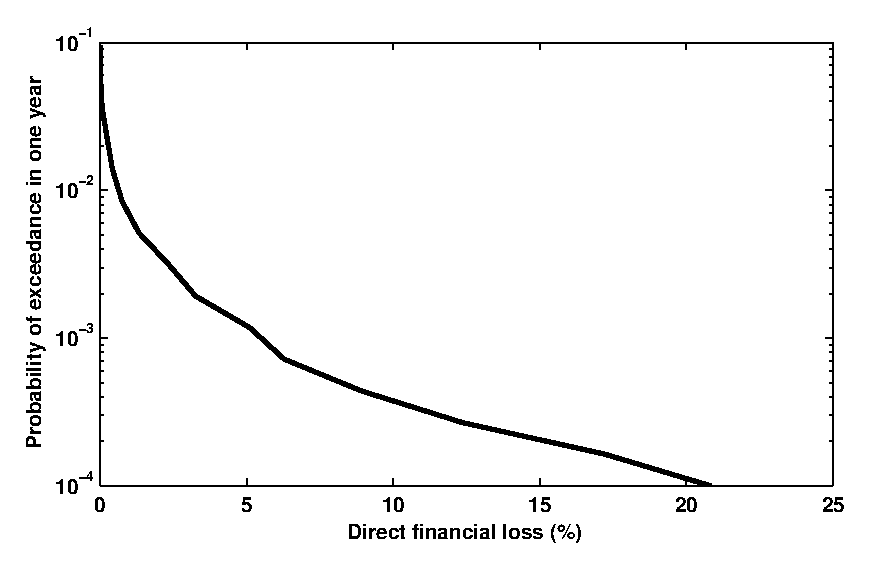
\includegraphics{fig-risk-pml}
\caption{Risk exceedance curve for all the buildings in the
Newcastle and Lake Macquarie portfolio.} \label{fig-risk-pml}
\end{figure}
\fref{fig-risk-pml} provides an example of a risk exceedance curve
for the Newcastle and Lake Macquarie portfolio. The EQRM post
processing tool \typefunc{wrap}{\_risk}{\_plots} can be used with
the individual plotting tool \typefunc{pl}{ot\_}{pml} to plot a
risk exceedance curve.

\subsection{Annualised loss}

The annualised loss represents the loss per year averaged over all
of the synthetic earthquakes. It can be computed by integrating
underneath the risk exceedance curve. Since this is not
necessarily intuitive the proof is given below.

Consider the risk exceedance curve as the probability of a loss
being exceeded in a one year time frame $P(Y \ge y)$. Let
$f_{E_L}(\ell)$ denote the PDF (probability density function) of
the aggregate loss and $F_{E_L}(\ell)$ denote the CDF (cumulative
distribution function). Let us define $F_{E_L}(\ell)$ as the CDF,
$$
 F_{E_L}(\ell) = \int_0^\ell f(x)\, dx.
$$
and $G(\ell)$ as the exceedence probability function,
$$
 G_{E_L}(\ell) = 1 - F_{E_L}(\ell) = \int_\ell^\infty f_{E_L}(y)\,dy.
$$
The mean of the random variable $E_L$ or annualised loss is given
by the expectation
$$
 E(L) = \int_0^\infty y f_{E_L}(y)\,dy.
$$
Using integration by parts, and using $f_{E_L}(y) =
-G'_{E_L}(\ell)$, we get
$$
 E(L) = \int_0^\infty -y G'_{E_L}(y)\,dy
      =  \big[ -yG_{E_L}(y)\big]_0^\infty + \int_0^\infty
      G_{E_L}(y)\,dy.
$$

Assuming $xG_{E_L}\to 0$ as $x\to\infty$ (which is true for an
exponential distribution, or distribution which behaves
asymptotically as exponential) we have
$$
 E(L) = \int_0^\infty G_{E_L}(y)\,dy
$$
which demonstrates that the mean value of the loss is the area
under the risk exceedance curve (PML).

The EQRM post processing tool \typefunc{wrap}{\_risk}{\_plots} can
be used with the individual plotting tool
\typefunc{calc}{\_ann}{loss} to compute the annualised loss.The
annualised loss associated with the PML in \fref{fig-risk-pml} is
0.03\%.

\subsection{Disaggregated annualised loss}

Storing the loss results for all of the earthquake-building pairs
allows the de-aggregation of annualised loss into a range of
classes. The EQRM offers several tools to assist the
de-aggregation into common classes all of which are managed
through the plotting tool \typefunc{wrap}{\_risk}{\_plots}. These
are described as follows:
\begin{figure}
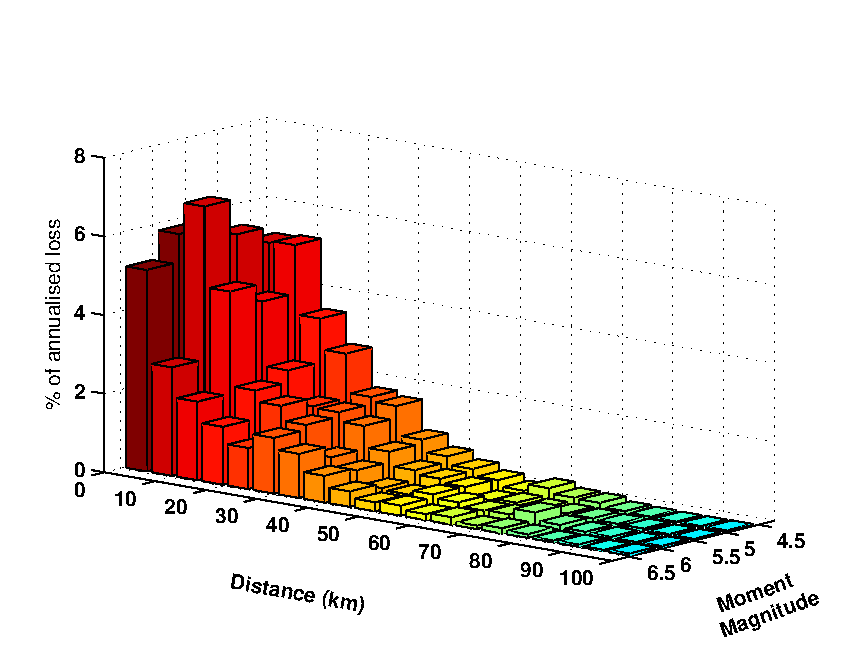
\includegraphics{fig-risk-deaggdistmag}
 \caption{Annualised loss
disaggregated by distance and magnitude for the Newcastle and Lake
Macquarie region.} \label{fig-risk-deaggdistmag}
\end{figure}
\begin{figure}
\includegraphics{fig-risk-deaggstruct}
\caption{Annualised loss disaggregated by building construction
type for the Newcastle and Lake Macquarie region.}
\label{fig-risk-deaggstruct}
\end{figure}
\begin{enumerate}
\item \textbf{disaggregation by distance and magnitude} allows the
visualisation of magnitude-distance combinations which have the
greatest influence on risk assessments.
\fref{fig-risk-deaggdistmag} illustrates the disaggregation by
distance and magnitude for risk in the Newcastle and Lake
Macquarie region. The individual plotting tool
\typefunc{calc}{\_annloss}{\_deagg\_distmag} can be used with
\typefunc{wrap}{\_risk}{\_plots} to de-aggregate the risk by
distance and magnitude. \item \textbf{disaggregation by building
construction type} separates the annualised loss into the four
major construction types; wood framed, un-reinforced masonry,
concrete and steel framed. \fref{fig-risk-deaggstruct} illustrates
the annualised loss disaggregated by structural type for the
Newcastle and Lake Macquarie region. The individual plotting tool
\typefunc{calc}{\_annloss}{\_deagg\_structural} can be used with
\typefunc{wrap}{\_risk}{\_plots} to de-aggregate the risk by
structural type. \item \textbf{disaggregation by suburb} separates
the annualised loss into different suburbs and allows the
visualisation of how earthquake risk varies spatially. The
individual processing tool
\typefunc{calc}{\_annloss}{\_deagg\_sub} can be used with
\typefunc{wrap}{\_risk}{\_plots} to de-aggregate the risk by
suburb. Note that \typefunc{calc}{\_annloss}{\_deagg\_sub}
produces a CSV file that can be plotted in GIS or some other
environment.
\end{enumerate}

\section{Earthquake scenario results}

The output for an earthquake scenario loss simulation is also
stored in the file
\typeoutput{<site\_loc>}{\_db\_saved}{ecloss}{.mat}. The format
for this file is exactly the same as the format for the
probabilistic risk output. Note, however, that each of the
earthquakes in \typeoutput{<site\_loc>}{\_db\_saved}{ecloss}{.mat}
represent different realisations of the same scenario (see
\sref{sec:source-scenario}).
\begin{figure}
\includegraphics{fig-risk-scen-hist}
\caption{Histogram of loss estimates for a synthetic Newcastle
1989 earthquake.} \label{fig:scenario-hist}
\end{figure}
The primary technique for visualising an EQRM scenario output is
via a histogram such as that shown in \fref{fig:scenario-hist} for
a simulation of the Newcastle 1989 earthquake. Each bar of the
histogram in \fref{fig:scenario-hist} represents the frequency of
realisations which predicted a loss value within the bars domain.
Histograms such as \fref{fig:scenario-hist} can be produced using
the individual plotting tool
\typefunc{calc\_scen}{\_loss}{\_stats} with
\typefunc{wrap}{\_risk}{\_plots}. Note that
\typefunc{calc\_scen}{\_loss}{\_stats} also produces basic
statistics for the scenario realisations such as the mean and
median.



\section{Key functions, flags and parameters}

\begin{tabular}{llp{0.5\textwidth}}
\hline
\textbf{Name} & \textbf{Type} & \textbf{Description} \\
\hline
\keyrowsep \typeoutput{<site\_loc>}{\_db}{\_hzd}{.mat} & Output& EQRM output file for a probabilistic earthquake hazard run.\\
\keyrowsep \splitrowoutput{<site\_loc>\_db}{\_savedecloss}{.mat} & Output & EQRM output file for a probabilistic (or scenario) risk run. \\
\keyrowsep \typepar{rtrn}{\_}{per} & Par & Vector whose elements represent the return periods to be considered. \\
\keyrowsep \typefunc{plot}{\_hzd}{\_map} & Function& Post processing tool for plotting probabilistic earthquake hazard maps.\\
\keyrowsep \typefunc{create}{\_gis}{\_output} & Function & Post processing tool to export probabilistic earthquake hazard data.\\
\keyrowsep \typefunc{plot}{\_singlesite}{\_hzd} & Function & Post processing tool for plotting hazard exceedance curves or uniform hazard spectra.\\
\keyrowsep \typefunc{wrap}{\_risk}{\_plots} & Function & Post processing tool to handle user interaction with risk processing/plotting tools. \\
\keyrowsep \typefunc{pl}{ot\_}{pml} & Function & Post processing tool for plotting and computing the PML.\\
\keyrowsep \typefunc{calc}{\_ann}{loss} & Function & Post processing tool for computing the annualised loss.\\
\keyrowsep \splitrowfunc{calc\_annloss\_deagg}{\_distmag} & Function& Post processing tool for plotting the annualised loss disaggregated by distance and magnitude.\\
\keyrowsep \splitrowfunc{calc\_annloss\_deagg}{\_structural} & Function & Post processing tool for plotting the annualised loss disaggregated by building structural type.\\
\keyrowsep \splitrowfunc{calc\_annloss\_deagg}{\_sub} & Function & Post processing tool for computing the annualised loss disaggregated by suburb.\\
\keyrowsep \typefunc{calc\_scen}{\_loss}{\_stats} & Function & Post processing tool for analysing and plotting loss data for earthquake scenario runs.\\
 \hline
\end{tabular}


\appendix
\chapter{Appendicies}

\section{A selection of GMPE formulae}
\label{app:GMPE_eqns}

This appendex discusses individual GMPE's described in the previous
version of the EQRM manual.  This does not represent all of the GMPE's
available for use within EQRM, but rather a subset of the available
models.


\subsection{Toro ground motion formula}

The \citet{dr_Toro97a} ground motion relation used in the EQRM code
is based on the Joyner-Boore distance $\Rjb$ and moment-magnitude.
Note that this reference largely describes the variability and not
how the coefficients were derived. \citet{dr_EPRI93a} describes
how the coefficients were derived.

The \citet{dr_Toro97a} ground motion model divides North America
into two regions (Gulf and Mid-Continent) and can  be used with
two different measures of magnitude (local and moment). Currently
the EQRM can only use the Mid-Continent -- moment magnitude
version of the ground motion model. This version of the ground motion
model is used because the earthquake mechanism in Mid-Continent
USA is believed to be similar to that in Australia (i.e. both are
intraplate settings).

The ground motion formula is
\begin{equation}
\begin{split}
\mu_{log(S_a)}(T_o,r_m,\Rjb) &= C_1 + C_2(r_m-6) + C_3(r_m-6)^2 - C_4\ln(R_M) \\
       &\quad  - (C_5-C_4)\max\left[\ln\left(\frac{R_M}{100}\right),0\right] -C_6R_M,
\end{split}
\end{equation}
where
\begin{equation}
 R_M = \sqrt{ \Rjb^2 + C_7^2 }.
\end{equation}

The coefficients used in the code, $C_1,\ldots,C_7$, are functions
of $T_o$ and are tabulated in \citet[Table 2]{dr_Toro97a}.

The `uncertainty parameter' ($\sigma_{log(S_a)}$) can be
decomposed as follows:
\begin{equation}
 \sigma_{log(S_a)}(T_o,r_m,\Rjb) =
 \sqrt{\sigma_a(T_o,r_m,\Rjb)+\sigma_e(r_m)}.
\end{equation}

The aleatory or random uncertainty $\sigma_a$ can be separated
into a source dependant component $\sigma_{a,r_m}$ (see
\citet[Table 3]{dr_Toro97a}) and a path dependant
component $\sigma_{a,\Rjb}$ (see \citet[Table 4]{dr_Toro97a}) as follows:
\begin{equation}
\label{eq:attn-toro-aleat} \sigma_a =
\sqrt{\sigma_{a,r_m}^2(T_o,r_m) + \sigma_{a,\Rjb}^2(T_o,\Rjb)}.
\end{equation}
The EQRM uses the aleatory uncertainty as defined by
\eref{eq:attn-toro-aleat}.

The epistemic or knowledge uncertainty $\sigma_e$ is dependant
upon source only, that is \mbox{$\sigma_e =\sigma_{e,r_m}$} (see
\citet[Page 48]{dr_Toro97a} or
\typefunc{attn}{\_preptoro}{\_epistemic}). Note that
$\sigma_{a,r_m}$ is a function of $T_o$ and $r_m$;
$\sigma_{a,\Rjb}$ is a function of $T_o$ and $\Rjb$; and
$\sigma_{e,r_m}$ is a function of $r_m$ only.

\subsection{Gaull ground motion formula}
\label{attn:atten-formula-Gaull}


The \citet{dr_Gaull90a} ground motion relation, as used in the EQRM
code, is based on hypocentral distance $\Rhyp$ and local magnitude
$r_{m_l}$.The Gaull ground motion model can be used to compute (i)
the mean of the logarithm of PGA $\mu_{log(PGA)}$ or (ii) the mean
of the logarithm of the Modified Mercalli Intensity
$\mu_{log(\Imm)}$. The formula is based on empirical intensity
data in the Australian region and the PGA extension created using
Papua New Guinea data. For the purpose of this ground motion model
the Australian region is divided into four sub-regions, Western
Australia, Southeastern Australia, Northeastern Australia and
Indonesia. The ground motion formulae is:
\begin{equation}
lnY = \ln a-c\ln \Rhyp + br_{m_l}
\end{equation}
where $a$, $b$ and $c$ are constants, $r_{m_l}$ is the local
magnitude of the rupture and $lnY$ represents $\mu_{log(PGA)}$ or
$\mu_{log(MMI)}$ depending on the value of the constants. The
constants are tabulated in \citet[Table 4]{dr_Gaull90a}.

Note that in the case of the \citet{dr_Gaull90a} ground motion model
(PGA version) there is no need to prepare the ground motion
coefficients because the ground motion model is only defined for
$T_o=0 sec$ (PGA). To compute $S_a(T_o,r_m,R)$ (more specifically,
$\mu_{log(S_a)}$), we can extend the $PGA$ estimate using the
Australian Standard Response Spectral Acceleration
\citep{dr_Standards93a}. 

\citet[Table 4]{dr_Gaull90a} tabulate the `uncertainty
parameter(s)' ($\sigma_{log(Y)}$) and indicate that they do not
depend on $r_{m_l}$ or $\Rhyp$. Furthermore, when extending the
PGA estimate to a complete $S_a$ it is assumed that
$\sigma_{log(S_a)}$ is not a function of $T_o$ and that
\begin{equation}
\sigma_{log(S_a)}(T_o) = \sigma_{log(PGA)}.
\end{equation}
Personal discussions with Brian Gaull (2002 and 2003) have
revealed that the following values of $\sigma_{log(Y)}$; 0.7 (for
PGA) and 0.925 (for $\Imm$) should be used in preference to the
published values of 0.28 and 0.37 respectively.


\subsection{Atkinson and Boore ground motion formula}

The \cite{dr_Atkinson97a} ground motion relation, as used in the
EQRM code, is based on hypocentral distance $\Rhyp$ and moment
magnitude $r_m$. The formula is
\begin{equation}
\mu_{log(S_a)}(T_o,r_m,\Rhyp) = C_1 + C_2(r_m-6) + C_3(r_m-6)^2
-ln(\Rhyp)-C_4\Rhyp.
\end{equation}
The coefficients used in the code, $C_1,\ldots,C_7$, are functions
of $T_o$ and are tabulated in \citet[Table 1]{dr_Atkinson97a}.

The uncertainty is dependant on $T_o$ only and is defined by
\citet{dr_Atkinson95b}. It represents aleatory uncertainty,
$\sigma_a$ and no attempt is made to separate it into into source
and path components (see \citealt[Table 2]{dr_Atkinson79a}).


\subsection{Sadigh ground motion formula}

The \cite{dr_Sadigh97a} ground motion relation, as used in the EQRM
code, is based on rupture distance $\Rrup$ and moment-magnitude
$r_m$. Using the convention defined by \citet{dr_Campbell03a} (in
accompanying appendix), the ground motion formula is
\begin{equation}
\begin{split}
\mu_{log(S_a)}(T_o,r_m,\Rrup) & = C_1F +C_2 + C_3r_m
+C_4(8.5-r_m)^2 + \\ c_5ln(r_{rup}+C_7\exp{c_8r_m}) +
C_6ln(r_{rup}+2),
\end{split}
\end{equation}
where the parameter $F$ is hard wired in the EQRM to 1 (hence
assuming reverse faulting). The coefficients used in the code,
$C_1,\ldots,C_7$, are functions of $T_o$ and $ r_m$. They are
tabulated in \citet[Table 2]{dr_Sadigh97a}.

\cite{dr_Sadigh97a} define a magnitude $r_m$ and period $T_o$
dependant `standard error' $\sigma(r_m,T_o)$ (see \citealt[Table
3]{dr_Sadigh97a}) which can be generalised as follows
\begin{equation}
\sigma(r_m,T_o) = \left \{ \begin{array}{ll}
C_{10}-C_{11}r_m & \textrm{for $0<r_m<7.21$} \\
c_{12} & \textrm{for $r_m \geq 7.21$} \\
\end{array} \right.
\end{equation}
where the coefficients $C_{10}$, $C_{11}$ and $C_{12}$ are
functions of $T_o$, and are defined in \cite[Table
A-14]{dr_Campbell03a}. For the purpose of
consistency, $\sigma(r_m,T_o)$ is assumed to be the aleatory
uncertainty $\sigma_a$.


\subsection{Somerville ground motion formula}
The \citet{dr_Somerville01a} ground motion relation, as used in the
EQRM code, is based on Joyner--Boore distance $R_{jb}$ and moment
magnitude $r_m$. The \citet{dr_Somerville01a} ground motion model
can be used for rift or nonrift zones and for vertical or
horizontal shaking (i.e. four seperate versions). The default
setting in the EQRM is nonrift.



The ground motion formula is
\begin{equation}
\begin{split}
\mu_{log(S_a)}(T_o,r_m,\Rjb) &= C_1 + C_2(r_m-6.4) + C_3ln(R_M) + C_4(r_m-6.4))\ln(R_M) \\
       &\quad  + C_5 \Rjb+ C_7(8.5-r_m)^2,
\end{split}
\end{equation}
for $\Rjb<50$, and
\begin{equation}
\begin{split}
\mu_{log(S_a)}(T_o,r_m,\Rjb) &= C_1 + C_2(r_m-6.4) + C_3ln(R_M) + C_4(r_m-6.4))\ln(R_M) \\
       &\quad  + C_5 \Rjb + C_6(ln(R_M)-ln\sqrt{2536}) +    C_7(8.5-r_m)^2,
\end{split}
\end{equation}
for $\Rjb \geq 50$, where
\begin{equation}
 R_M = \sqrt{ \Rjb + 6^2 }.
\end{equation}

The coefficients used in the code, $C_1,\ldots,C_7$, are functions
of $T_o$ and are tabulated in \citet[Table 9]{dr_Somerville01a}.

\cite{dr_Somerville01a} describe five types of uncertainty as
follows:

\begin{supertabular}{ll}
$\sigma_{\mu}$ & uncertainty in the median ground motion = 0.2. \\
$\sigma_{\sigma}$ & uncertainty in the scatter about median ground motion = 0.15. \\
$\sigma_{modeling}(T_o)$ & representing the discrepancy between
actual
physical processes \\
  & and the simplified representation of the model.\\
$\sigma_a(T_o)$ & arising from parameters varied in the study of \\
 & \cite{dr_Somerville01a}. \\
$\sigma_b(T_o)$ & arising from earlier studies by the same
authors.\\
\end{supertabular}

The terms $\sigma_{\mu}$ and $\sigma_{\sigma}$ are clearly
epistemic uncertainty. \cite{dr_Somerville01a} then define
$\sigma_{modeling}(T_o)$, $\sigma_a(T_o)$ and $\sigma_b(T_o)$ as
contributions to the scatter and as such the aleatory uncertainty
is taken to be:
\begin{equation}
\sigma_{a,log(S_a)}(T_o) = \sqrt{
\sigma_{modeling}^2(T_o)+\sigma_a^2(T_o)+\sigma_b^2(T_o) }.
\end{equation}

\
\eject






\small
\bibliography{drrefs,garefs,EQRM_refs}
%\bibliography{eqrmtech.bbl}
\printindex

\end{document}
